\newgeometry{textwidth=16cm}
\chapter[Vibrational spectra calculations]{Heteroatoms}
\minitoc
\restoregeometry

\newpage
	
	
	\section*{Introduction}


The chemical complexity of asphaltenes, which represent the heaviest fraction of oil, make their analysis and modelling very challenging, since the detailed molecular composition remains up to now unknown. However, some studies have reported that they consist of a heterogeneous mixture of polycondensed molecules, containing heteroatoms $X$ such as sulfur, oxygen, and nitrogen. On the other hand, vibrational spectroscopy has shown to be a tool for the identification and characterization of molecules in ill-defined mixtures, in combination with predictive modelling.\\

Considering this, in this chapter, the far- and mid-infrared spectra of a series of heteroaromatic (N, O and S) hydrocarbons and their dimers have been calculated using Density Functional Theory (DFT) within the $\omega$B97X-D/6-311++G** level of theory. The perturbational-variational method presented in the previous chapter coupled with potential truncation was incorporated in order to provide anharmonic corrections of monomers. Identification and quantification of peaks from \textit{inter} and \textit{intra}-molecular vibrations in experimental spectra have been performed. Also, experimental IR bands in the far-IR region were identified, allowing the differentiation of the \textit{inter}-molecular and \textit{intra}-molecular vibrations. In addition, the interaction energies were studied using DFT-SAPT\footnote{The symmetry-adapted perturbation theory based on density functional theory) at the PBE0/aug-cc-pVTZ level of theory.} \\
	
	These methods reproduce energies in the same order of magnitude and identify $\pi-\pi$ stacking as the dominant electronic interaction. Understanding the interaction between these primary units helped us to enrich the knowledge of the \textit{inter} and \textit{intra}molecular interactions in asphaltenes and why they tend to aggregate and then flocculate from the oil condensed phase. This outcome illustrates that the spectral signatures of heteroaromatic compounds can be used to probe the molecular and sub-molecular composition, and the \textit{inter}-molecular interactions present in asphaltenes by spectral decomposition.\\
	
	
	\section{Structural details}
	
	The molecular structures of thiophene, benzofuran, carbazole and fluorene-like molecules and their respective dimers were calculated using Density Functional Theory (DFT) with the $\omega$B97X-D exchange-correlation functional and the   6-311++G** basis set, implemented in the Gaussian 09 suite of programs. The $\omega$B97X-D functional developed by Chai \textit{et al}\cite{chai2008systematic} is based on optimized long-range corrected hybrid density functionals, which employ 100\% Hartree-Fock (HF) exchange for long-range electron-electron interaction correction. This method, tested by Salzner \textit{et al}\cite{salzner2011improved} for $\pi$-conjugated oligomers, was also benchmarked successfully for interacting polycondensed aromatic molecules,\cite{spillebout2014discerning} thus proving it overcomes the failure of standard DFT calculation approaches to describe long-distance interactions. The 6-311++G** basis set is of triple-zeta quality for the valence electrons. Among the basis sets tested by Wiberg,\cite{wiberg2004basis} including the Dunning correlation basis sets such as aug-cc-pVTZ and aug-cc-pVQZ, the 6-311++G** basis set gave accurate geometries and frequencies at a relatively small computational cost. The geometrical parameters of the molecules are benchmarked with experimental data when available.\\
	
	
	For dimers, as an alternative to the supermolecular treatment, an approach based on symmetry-adapted perturbation theory (SAPT)\cite{jeziorski1994perturbation} which utilizes the description of the interacting monomers in terms of Kohn-Sham (KS) orbitals was used in this work. The DFT-based SAPT approach,\cite{hesselmann2005density} denoted herein as SAPT-DFT, is exact for all major components of the interaction energy (asymptotically for exchange interactions) in the sense that these energies would be exact if the DFT description of the monomers were exact. The SAPT-DFT calculations were performed using the MOLPRO2012 package.\cite{MOLPRO_brief} The PBE0 functional\cite{adamo1999toward} was used as a monomer DFT functional in SAPT, using the aug-cc-pVTZ basis set. 
	
\section{Results and Discussion}


\subsection{Global analysis}

The methodology behind this part of the work is close to that of the ‘design of experiments’ \cite{goupy2013introduction}. Indeed, studying all the moieties, all the heteroatoms, all the substituents as well as all the allowed \textit{inter}-molecular associations of the hypothetical constituents of the asphaltenes (for which, \textit{cf.} chapter 1, both the composition and formulation are unknown) is utopic and unrealistic. The general principles behind the approaches of the type “design of experiments” rely on the organisation and limitation of the experiments/calculations when a link between a response function $y$ and variables $x_i$ (designated a ‘factor’) is sought after. Within the context of this work, the searched response function is knowing whether or not, for any given compound constituted of a given moiety, presenting or not an heteroatom, interacting or not among them, owns an active vibrational signature. These three criteria represent the three principle factors taken into account in our calculations. Unluckily, our problem is more complex since, besides being active, this vibrational mode should also be identifiable within a spectral zone where the density of modes is weak enough to avoid hiding the signature that is looked for. The notion of spectral zone is the last factor that has been considered in this study.\\

Actually, we also could have multiplied the chemical moieties \textit{ad infinitum} and accumulate more and more vibrational information for these systems, but it would be very complicated and hard to manage and explore all these data. We have chosen to concentrate on a strict domain of definition for which the main pieces of information are controlled so that useful information can be provided to spectroscopists:  “is it possible for a given asphaltene to use IR and Raman to characterise the presence of associated systems?” and, “is it possible to assign these signatures to the presence of the three main heteroatoms (oxygen, sulphur and nitrogen)?”\\


Infrared and Raman spectra of  indene \textbf{1\textit{a}}, fluorene \textbf{1\textit{b}}, benzofluorene \textbf{1\textit{c}}, cyclopentaphenanthrene \textbf{1\textit{d}}, 1-methylfluorene \textbf{1\textit{e}}, 1,8-dimethylfluorene \textbf{1\textit{f}},
indole \textbf{2\textit{a}}, carbazole \textbf{2\textit{b}}, benzocarbazole \textbf{2\textit{c}}, 4,5-iminophenanthrene \textbf{2\textit{d}}, 1-methylcarbazole\textbf{1\textit{e}}, 1,8-dimethylcarbazole \textbf{1\textit{f}},
benzofuran \textbf{3\textit{a}}, dibenzofuran \textbf{3\textit{b}}, benzonaphtofuran \textbf{3\textit{c}}, tribenzofuran \textbf{3\textit{d}}, 4-methyldibenzofuran\textbf{3\textit{e}}, 1,8-dimethyldibenzofuran \textbf{3\textit{f}},
benzothiophene \textbf{4\textit{a}}, dibenzothiophene \textbf{4\textit{b}}, benzonaphtothiophene \textbf{4\textit{c}}, tribenzothiophene \textbf{4\textit{d}}, 4-methyldibenzothiophene \textbf{4\textit{e}} and 4,6-dimethyldibenzothiophene \textbf{4\textit{f}} were studied in this work. In complement, the observed bands of the monomers are assigned using high level calculations based on anharmonic electrical and mechanical approximations. All computational outcomes are reported in the annexe C.
	
	\begin{figure}[H]
		\begin{center}
			\begin{tabular}{c c c}
				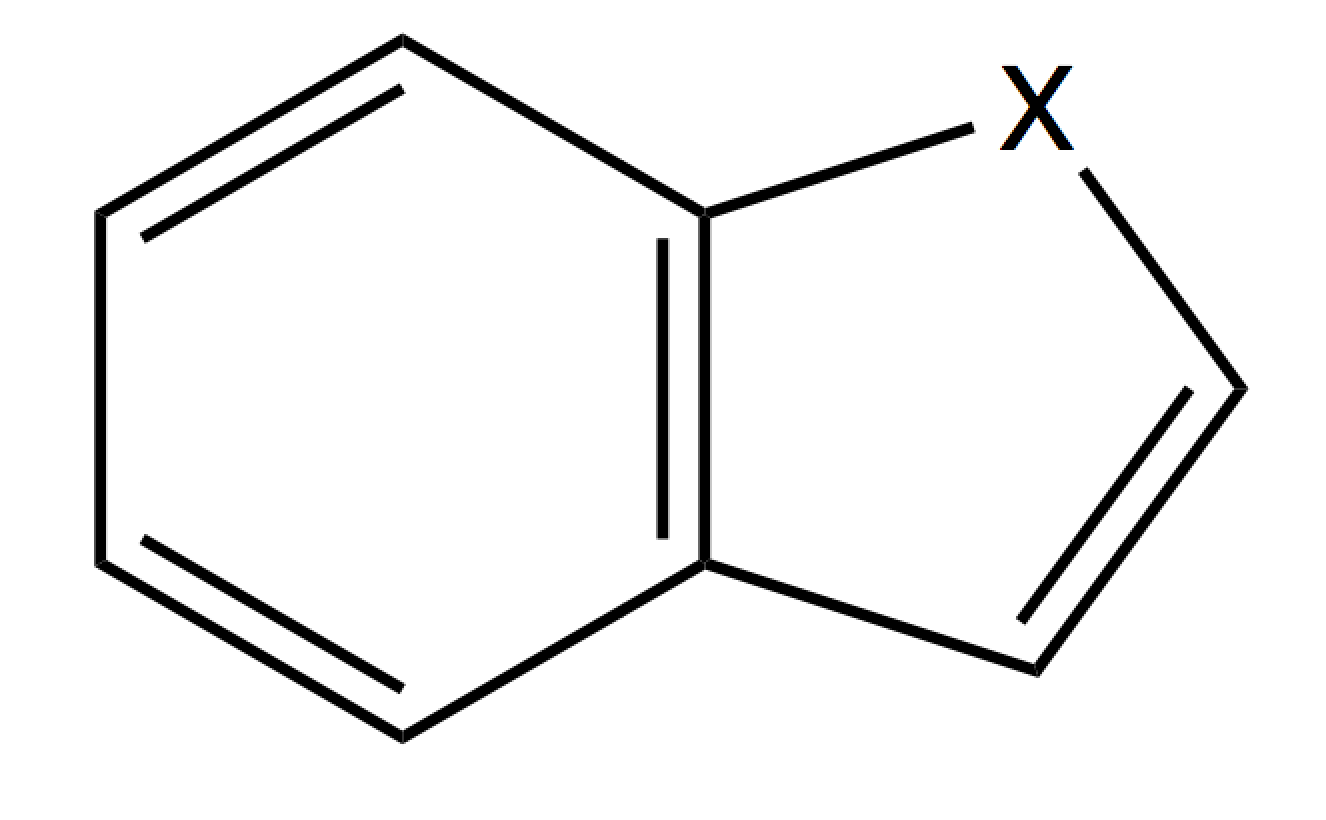
\includegraphics[scale=0.15]{image/benzo} & 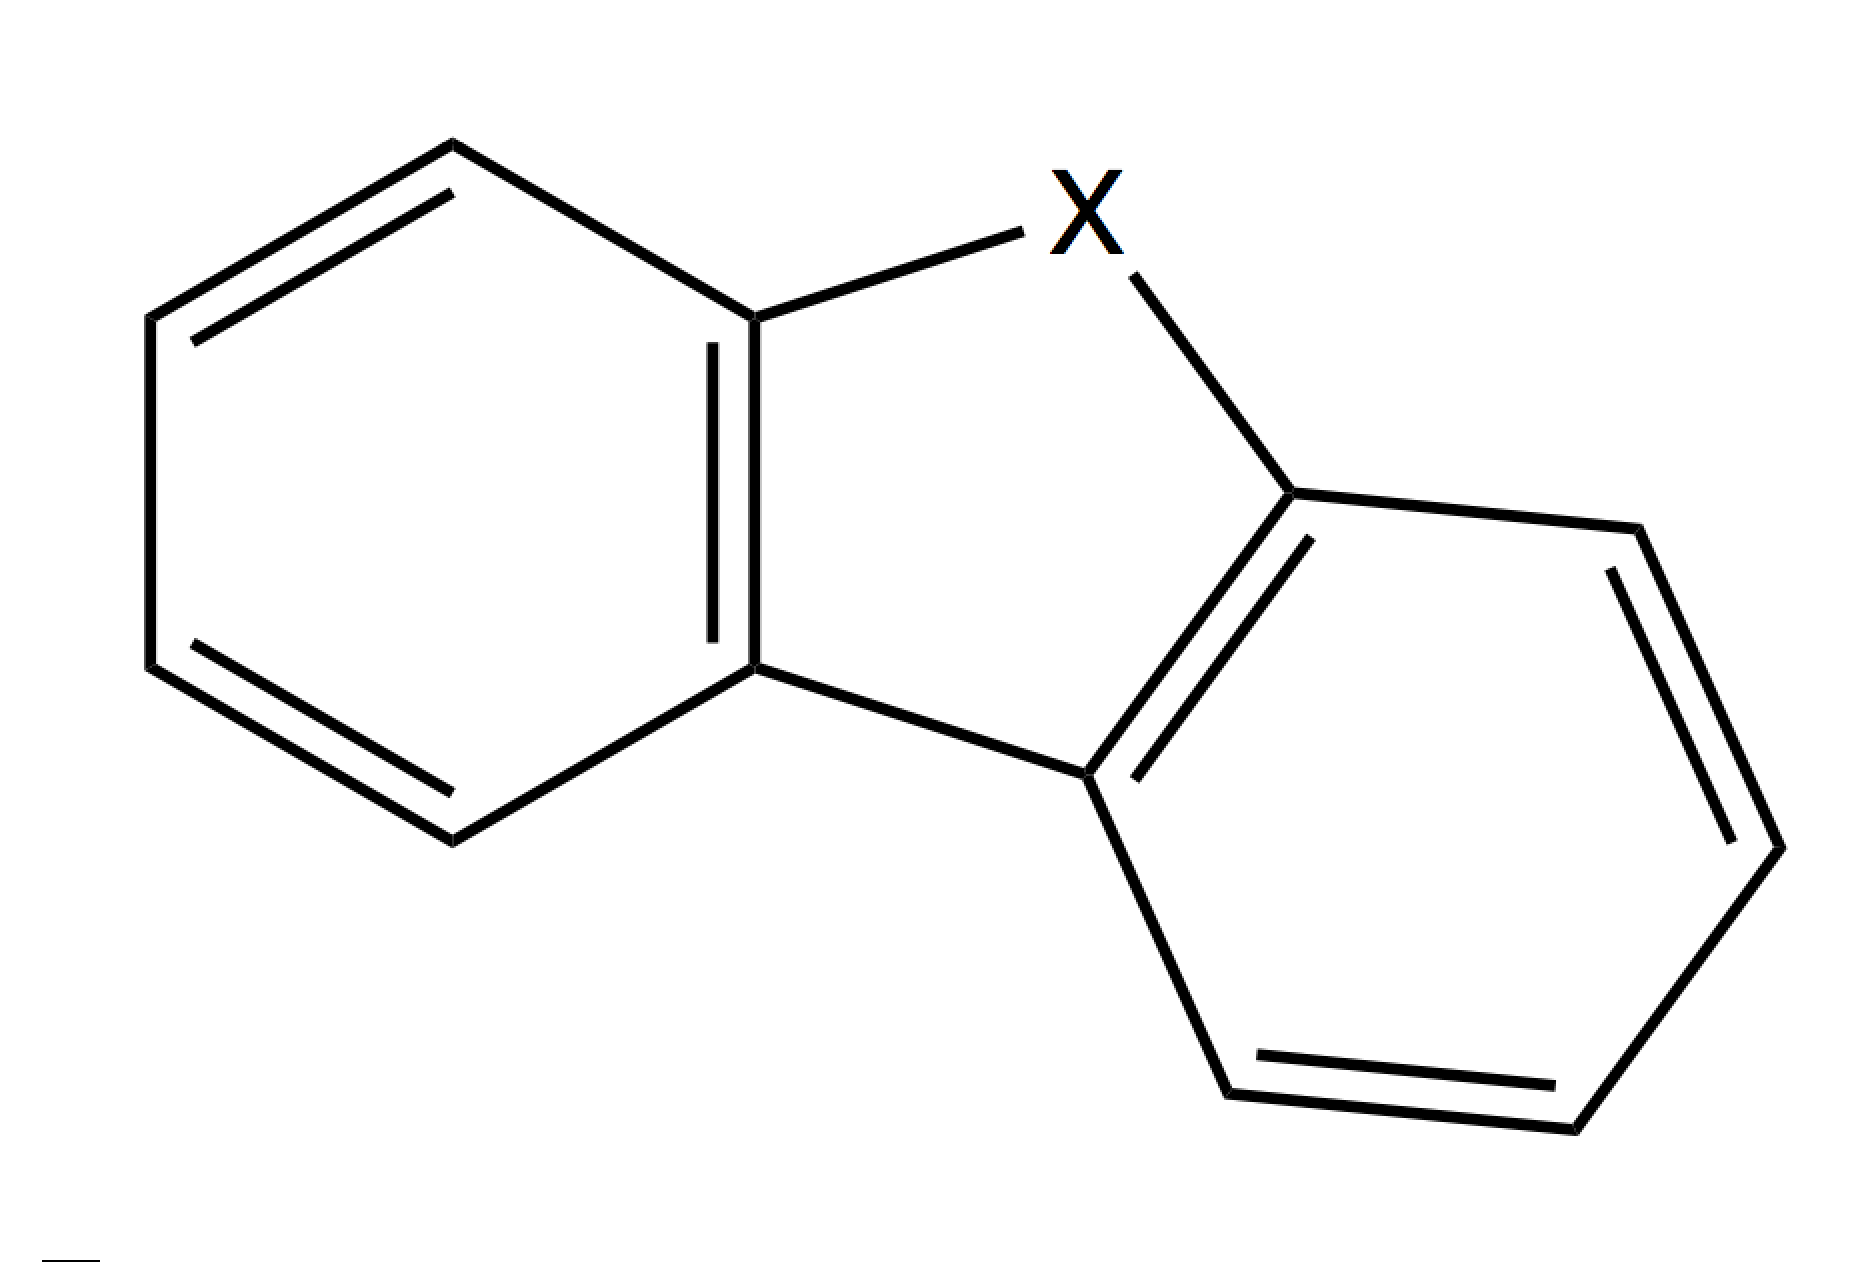
\includegraphics[scale=0.13]{image/dibenzo} & 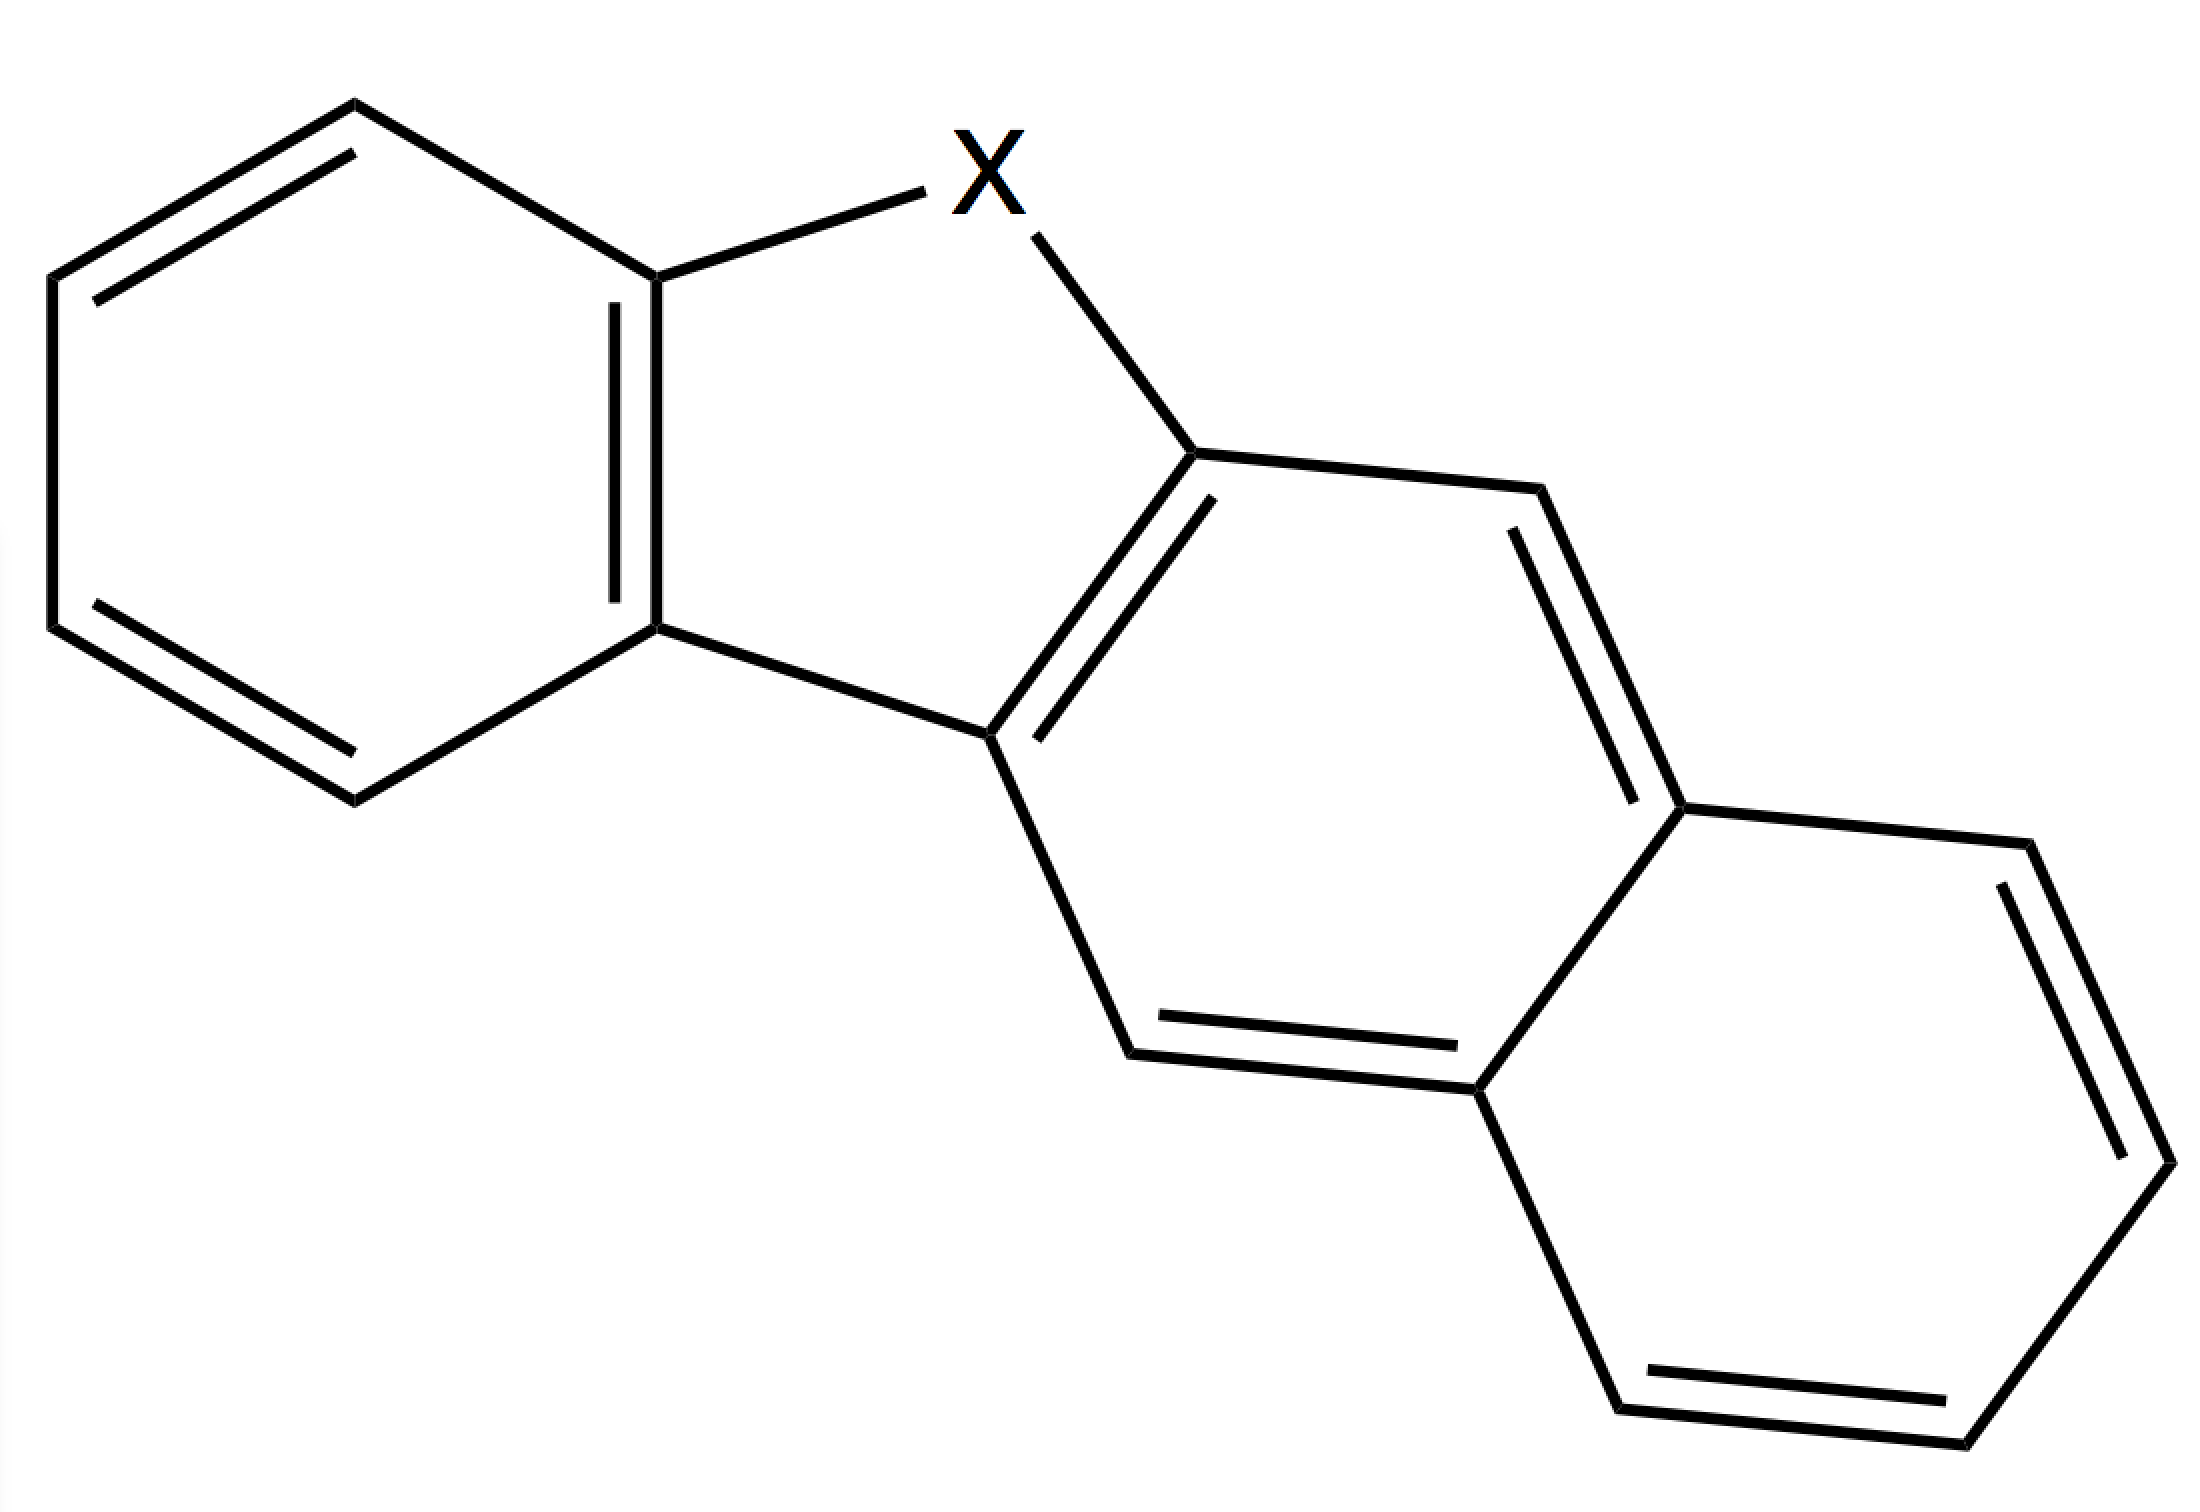
\includegraphics[scale=0.12]{image/benzonaphto}\\
				\textbf{1} & \textbf{2}& \textbf{3}\\
				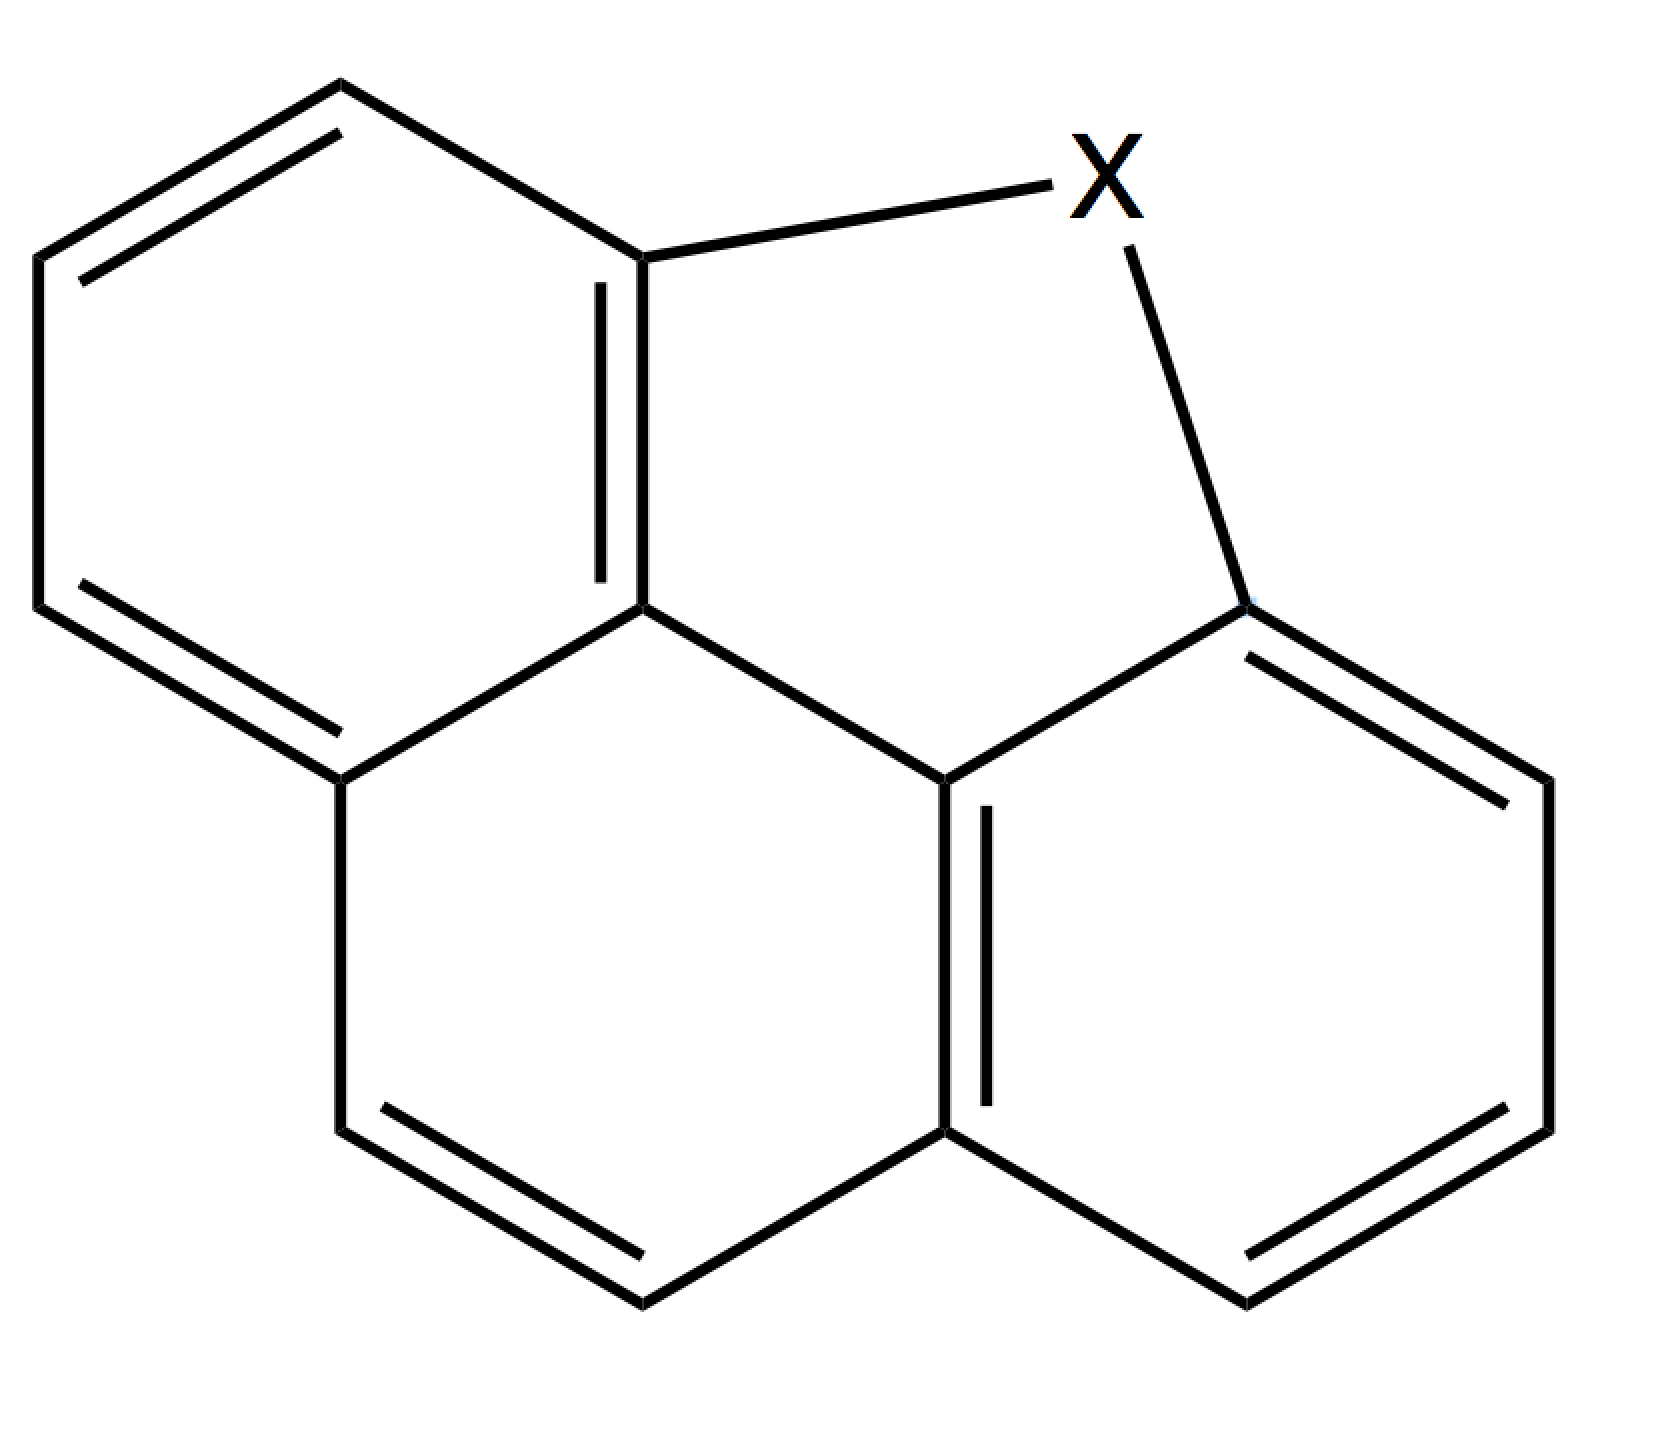
\includegraphics[scale=0.12]{image/tribenzo-lajolie} & 
				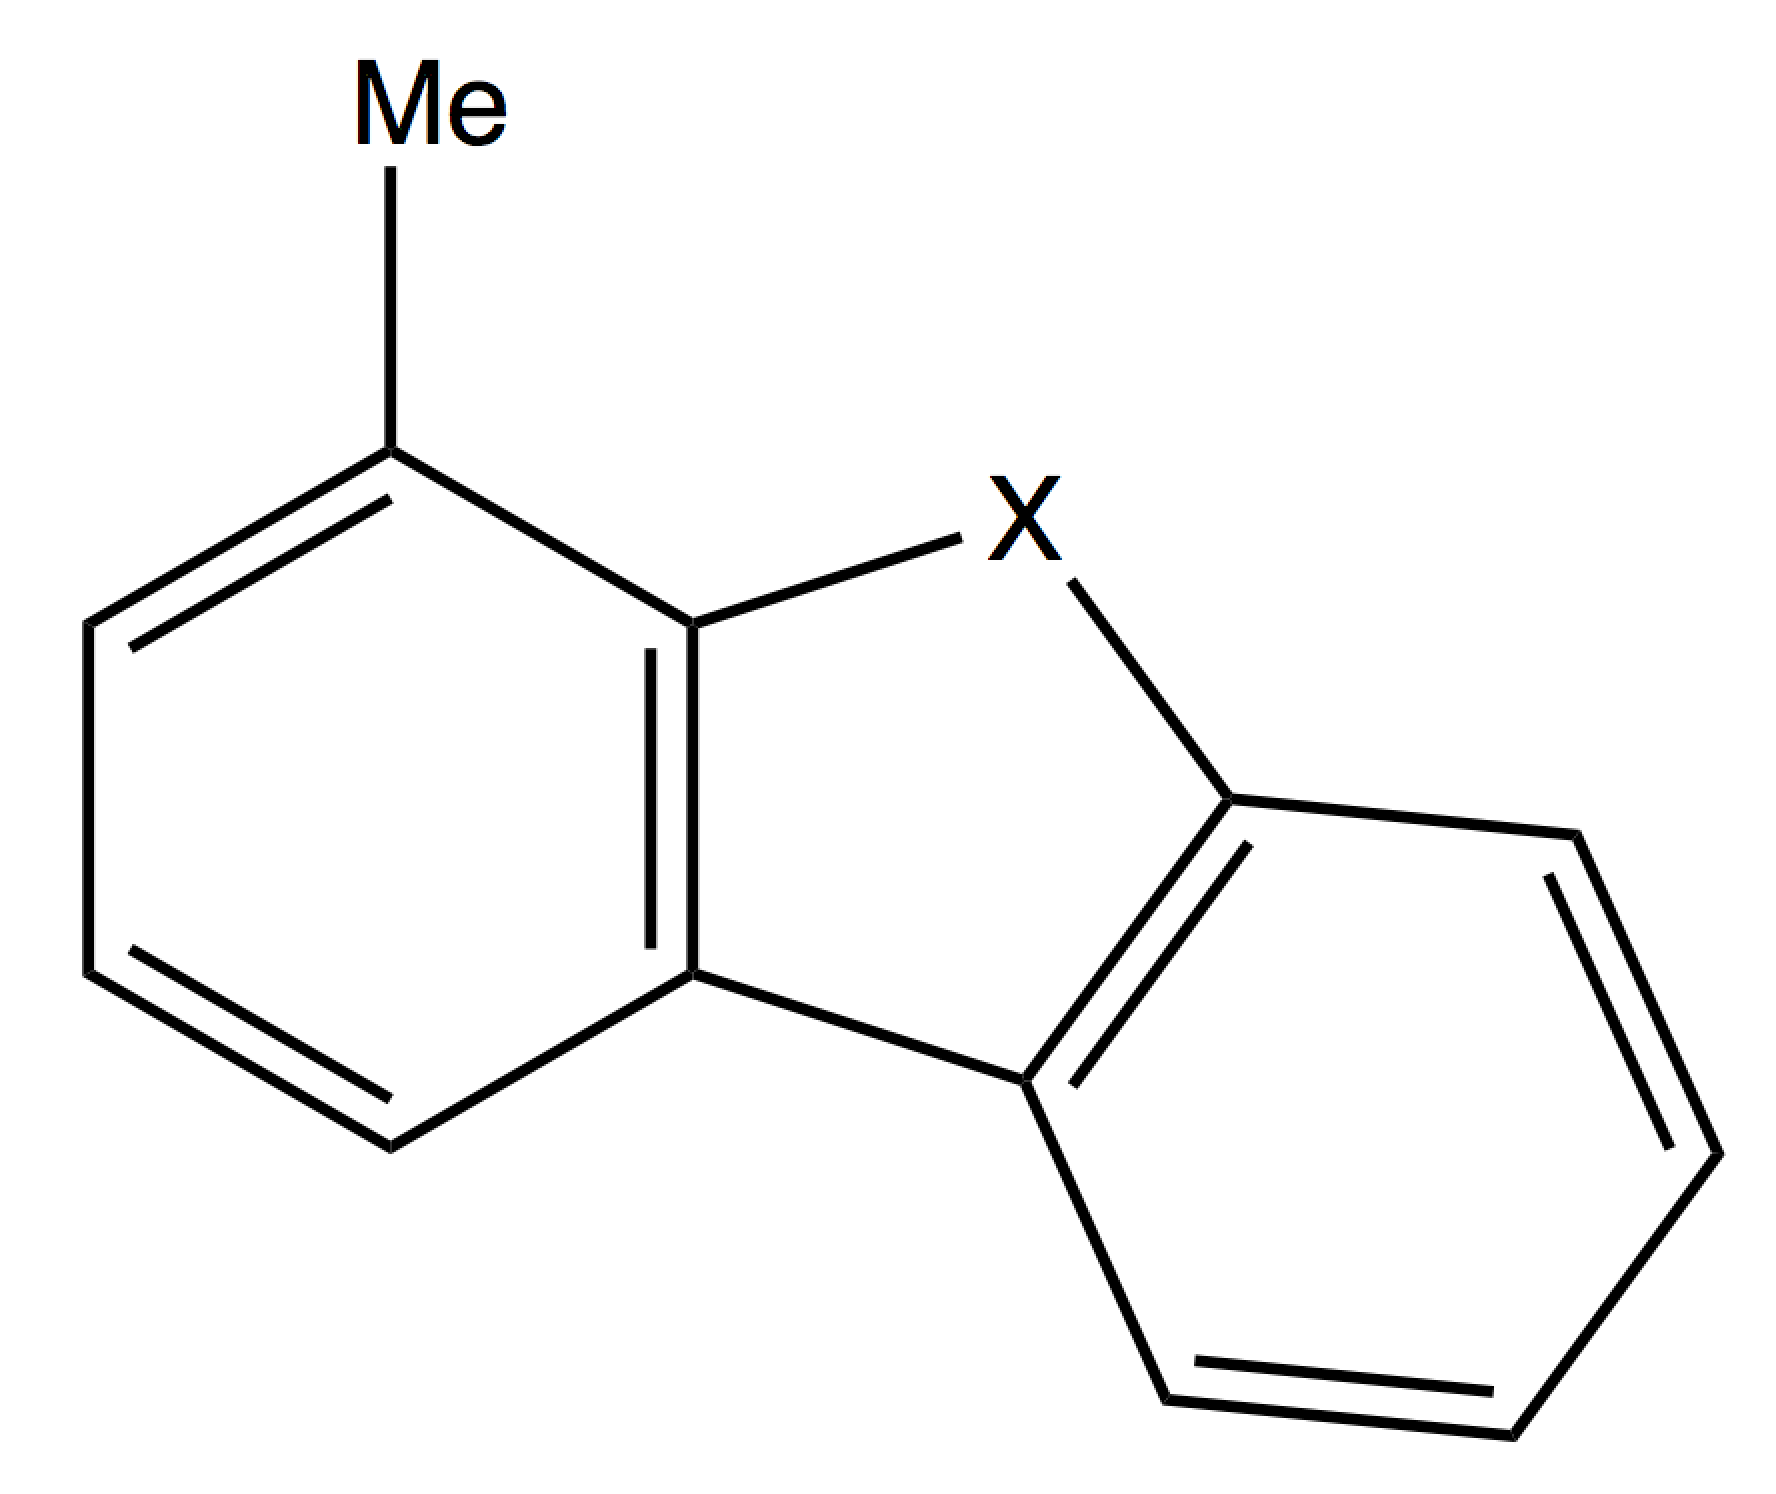
\includegraphics[scale=0.13]{image/methyl-benzo} & 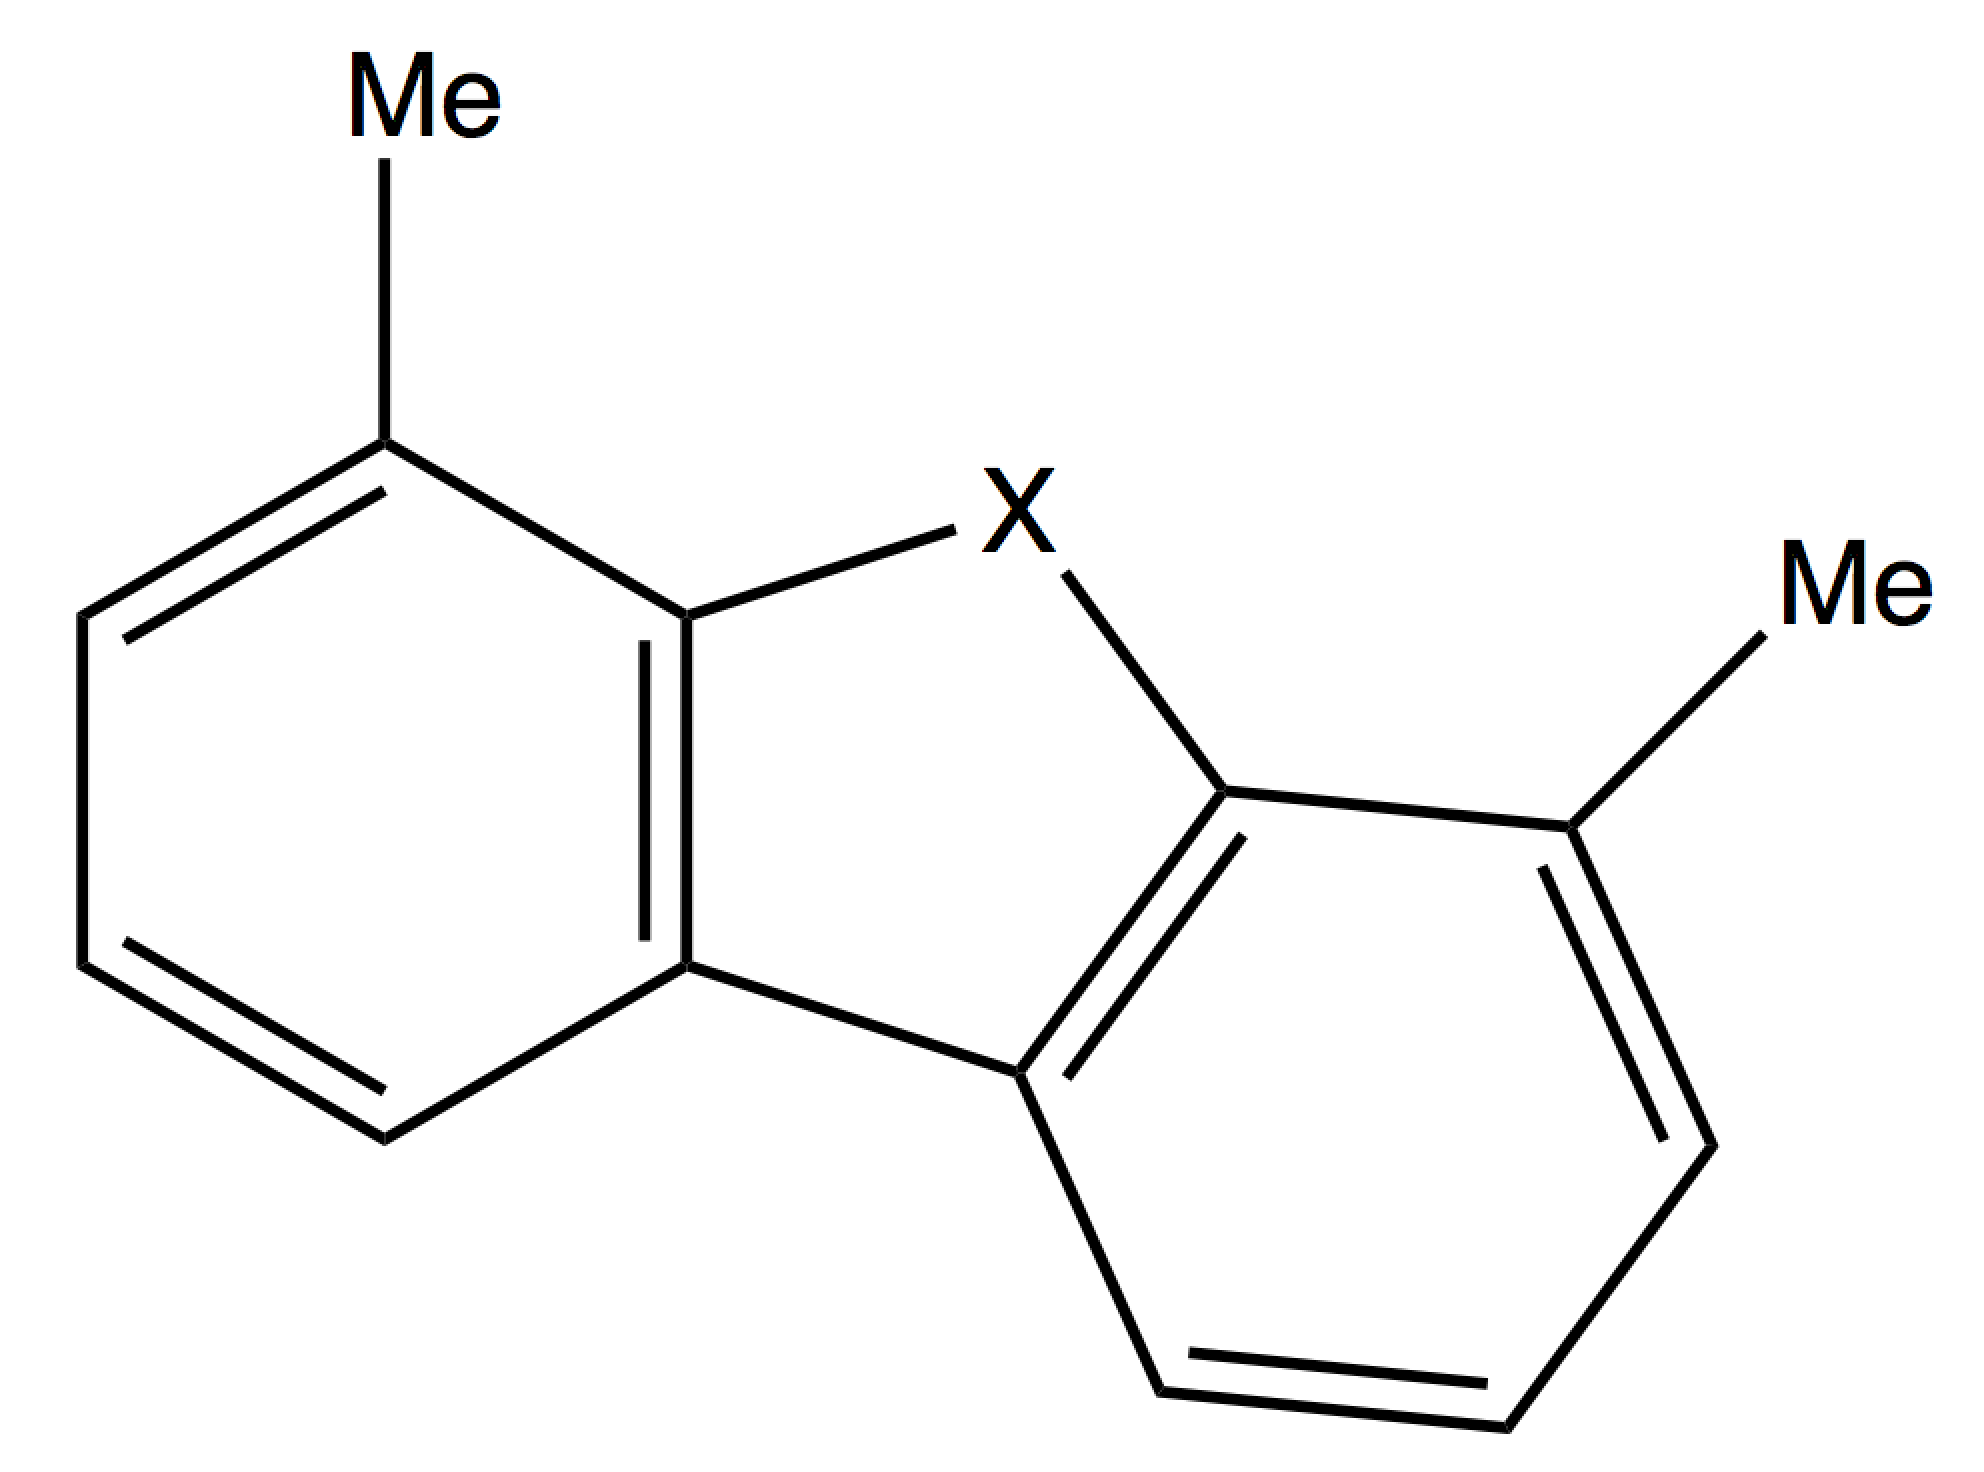
\includegraphics[scale=0.13]{image/dimethyl-benzo} \\
				\textbf{4} & \textbf{5} & \textbf{6}\\
			\end{tabular}
		\end{center}
		\caption{Molecular structures studied: \textbf{a} Benzo, \textbf{b} Dibenzo, \textbf{c} Benzonaphtho, \textbf{d} Tribenzo, \textbf{e} methyldibenzo, \textbf{f} dimethyldibenzo. X= \textbf{1} C, \textbf{2} N, \textbf{3} O and \textbf{4} S.}
	\end{figure}
	
	The two first factors we studied were: 1- the nature of the heteroatom (factor $x_1$), for which the bounds were arbitrarly set to $x_{1(min)}=C$ and $x_{1(max)}=S$; 2- the nature of the chemical moeity, which is discrete and not easily quantifiable ($x_{2(min)}=benzo$ and $x_{2(max)}=tribenzo$.). The spectral zone is then a third factor to be considered and which definition is also discrete. 
	Four spectral zones were defined: the very low wavenumbers one ($x_{3(min)}=1$), which displays the signatures of the \textit{inter}-molecular modes (represented on the figures by the “$ + $” symbol), butterfly-like (“$\ocircle$”) and torsion (“$\triangle$ and $\lozenge$”) modes, which are particularly active in this region; another one ($x_3=2$), covering the signatures of the cycle breathing and scissoring (“$\lhd$”), twist (“$\triangledown$”) and wagging modes that are impacted by the presence of the hetero atom (pure: $\pentagon$, X-H: $\octagon$, wagging/carbon backbone wagging: $\square$); $x_3=3$ covering the C-X ($\varhexagon$) streching, the CCC and CXC angular deformations ($\bigstar$) modes of the aromatic cycles and the C-H wagging modes ones; and, finally, the $x_3=4$ zone covering carbon-carbon and C-H streching modes found beyond 1300 cm$^{-1}$.  A table summarizing the modes that are followed in this study as well as their respective symbols is presented in Figure XX. The modes of interest and which are represented in our Figures by the use of pictograms are the ones for which the hetero atom contribution is strong for the ensemble of the 24 studied molecules, in average. The last factor considered in this work concerns the presence ($x_{4(min)}=yes$) or not ($x_{4(max)}=no$) of \textit{inter}-molecular interactions by analysing the dimers and monomers, respectively. However, one should note that this chapter only reports the results of the work done in the molecular state for which the only aim is defining if it is relevant to consider one or several spectra signatures (\textit{intra}- and \textit{inter}-molecular) that could allow one to characterise the heteroatoms present in the asphaltene mixtures and their associated vibrational modes. In chapter 6, the description of the \textit{inter}-molecular modes will be discussed in more details by the development of solid state calculations taking into account this time of the global environment of the studied systems.\\
	
	The implementation of an “ordered” strategy able to take into account the characteristics discriminating spectroscopically all the systems is justified when one take a look at Figure \ref{figP2-2}. In this figure, the ensemble of the calculated modes of the 24-monomer systems is reported without distinction neither of the spectral zone nor the intensity. We can easily realise the extent of the data available to treat this problem. Only the modes for which the heteroatom is directly implied  in the development of a given vibration are reported in Figure \ref{figP2-2} as colored points.
	
	
	\begin{figure}[H]
		\begin{center}
			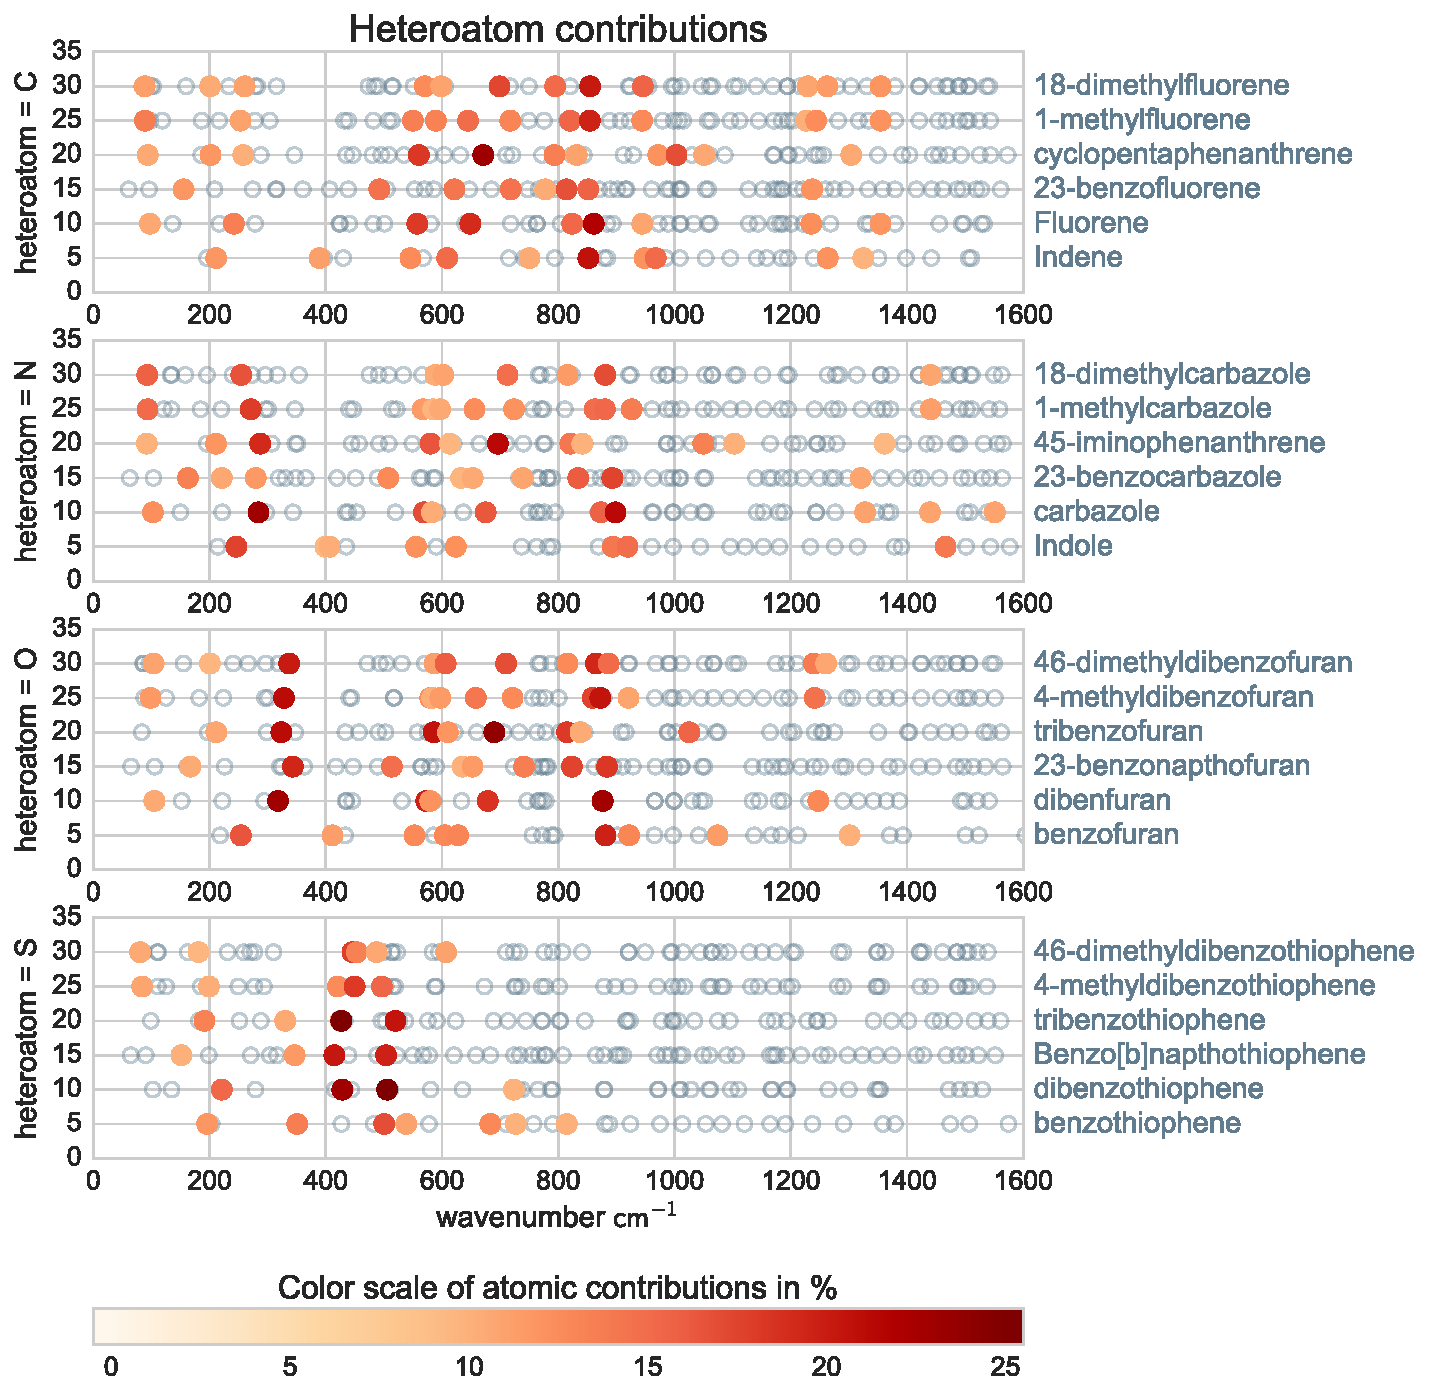
\includegraphics[scale=0.7]{image/P22}
		\end{center}
		\caption{Vibration modes heteroatoms contributions > 5\% for studied molecules.} \label{figP2-2}
	\end{figure}
	
Several pieces of informations can be extracted from this figure. First of all, the number of modes having an influence of the heteroatom X = C, N and O is of the order of 50\% of all the modes, regardless of the molecule. This percentage is reduced by half for the molecules of the thiophene family.The contributing modes are, in this case, concentrated in the low wavenumber spectral zones ($x_3=1$ and 2 – what is due to a simple mass effect). This first analysis also shows that within the three first spectral zones localised below 1300 cm$^{-1}$ there are much more similarities between the signatures of $x_1=N$ and $O$ heteroatoms than there are between $S$ and $C$. Lastly, and except for sulfur, it is clear that below 1000 cm$^{-1}$ the signature of each moiety is singular. This observation is particularly pronounced in the lowest spectral zone $x_3=1$, where the torsion and deformation modes of the backbone can be found (including, this time, the thiophenic molecules). The moiety seems to be, at this stage, a major discriminatory criterion of the spectral signature of these molecules. 
	
	
	
	
		\begin{figure}[H]
			\begin{center}
				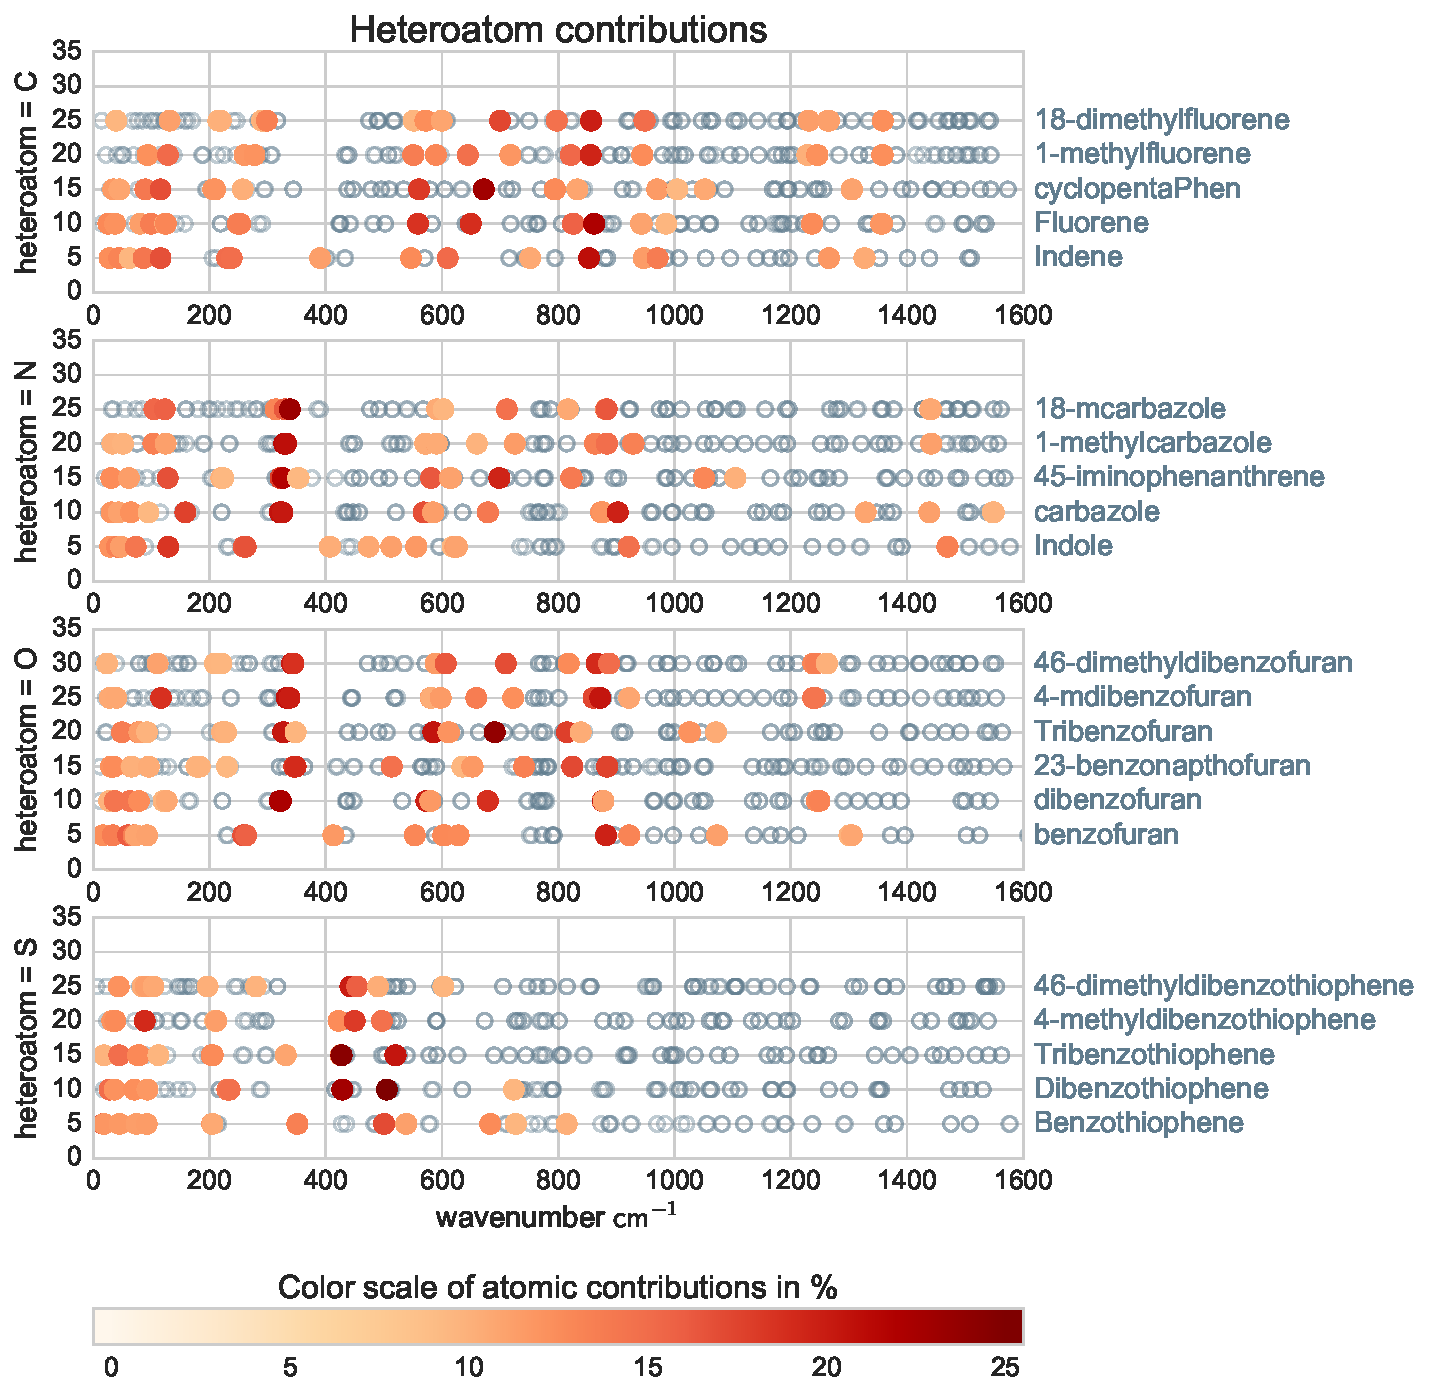
\includegraphics[scale=0.7]{image/P2-3}
			\end{center}
			\caption{Vibration modes heteroatoms contributions > 5\% for dimers configurations}  \label{figP2-3}
		\end{figure}
	
	
In figure \ref{figP2-3}, the same information reported in figure 2 is presented for the ensemble of the most stable dimer of each specie. Figure \ref{figP2-2} and \ref{figP2-3} look alike apart from the emergence of \textit{inter}-molecular modes at very low wavenumbers for which the contribution of the hetero atoms are strong. Another remarkable difference concerns the nitrogen heteroatom since it seems that it is the only one with a density and rate of contributing modes evolving. This is particularly true for the zones $x_3=1$ around 150 cm$^{-1}$ and $x_3=2$ around 400-500 cm$^{-1}$. No other significant difference can be highlighted from figure \ref{figP2-3}. This corroborates the idea stating that the signatures of the \textit{intra}-molecular modes specific to each molecule constituting the dimers are, except these two precedent observations, the very same reported for the monomers. 
Another difference that can be noted is the spectral behaviour of the 24 molecules within the study domain depiced in Figure \ref{figP2-4}. In this figure the spectral signatures taking into account the intensities and filtrated by each moiety are reported. For each one of them, one can observe again at the lowest frequencies a singular behaviour of the signatures associated to the molecules of the carbazol family. The modes associated seem to own more intense signature for which the position seems to depend on the moiety more than for any other heteroatom.	
	
	
	\begin{figure}[H]
		\begin{center}
			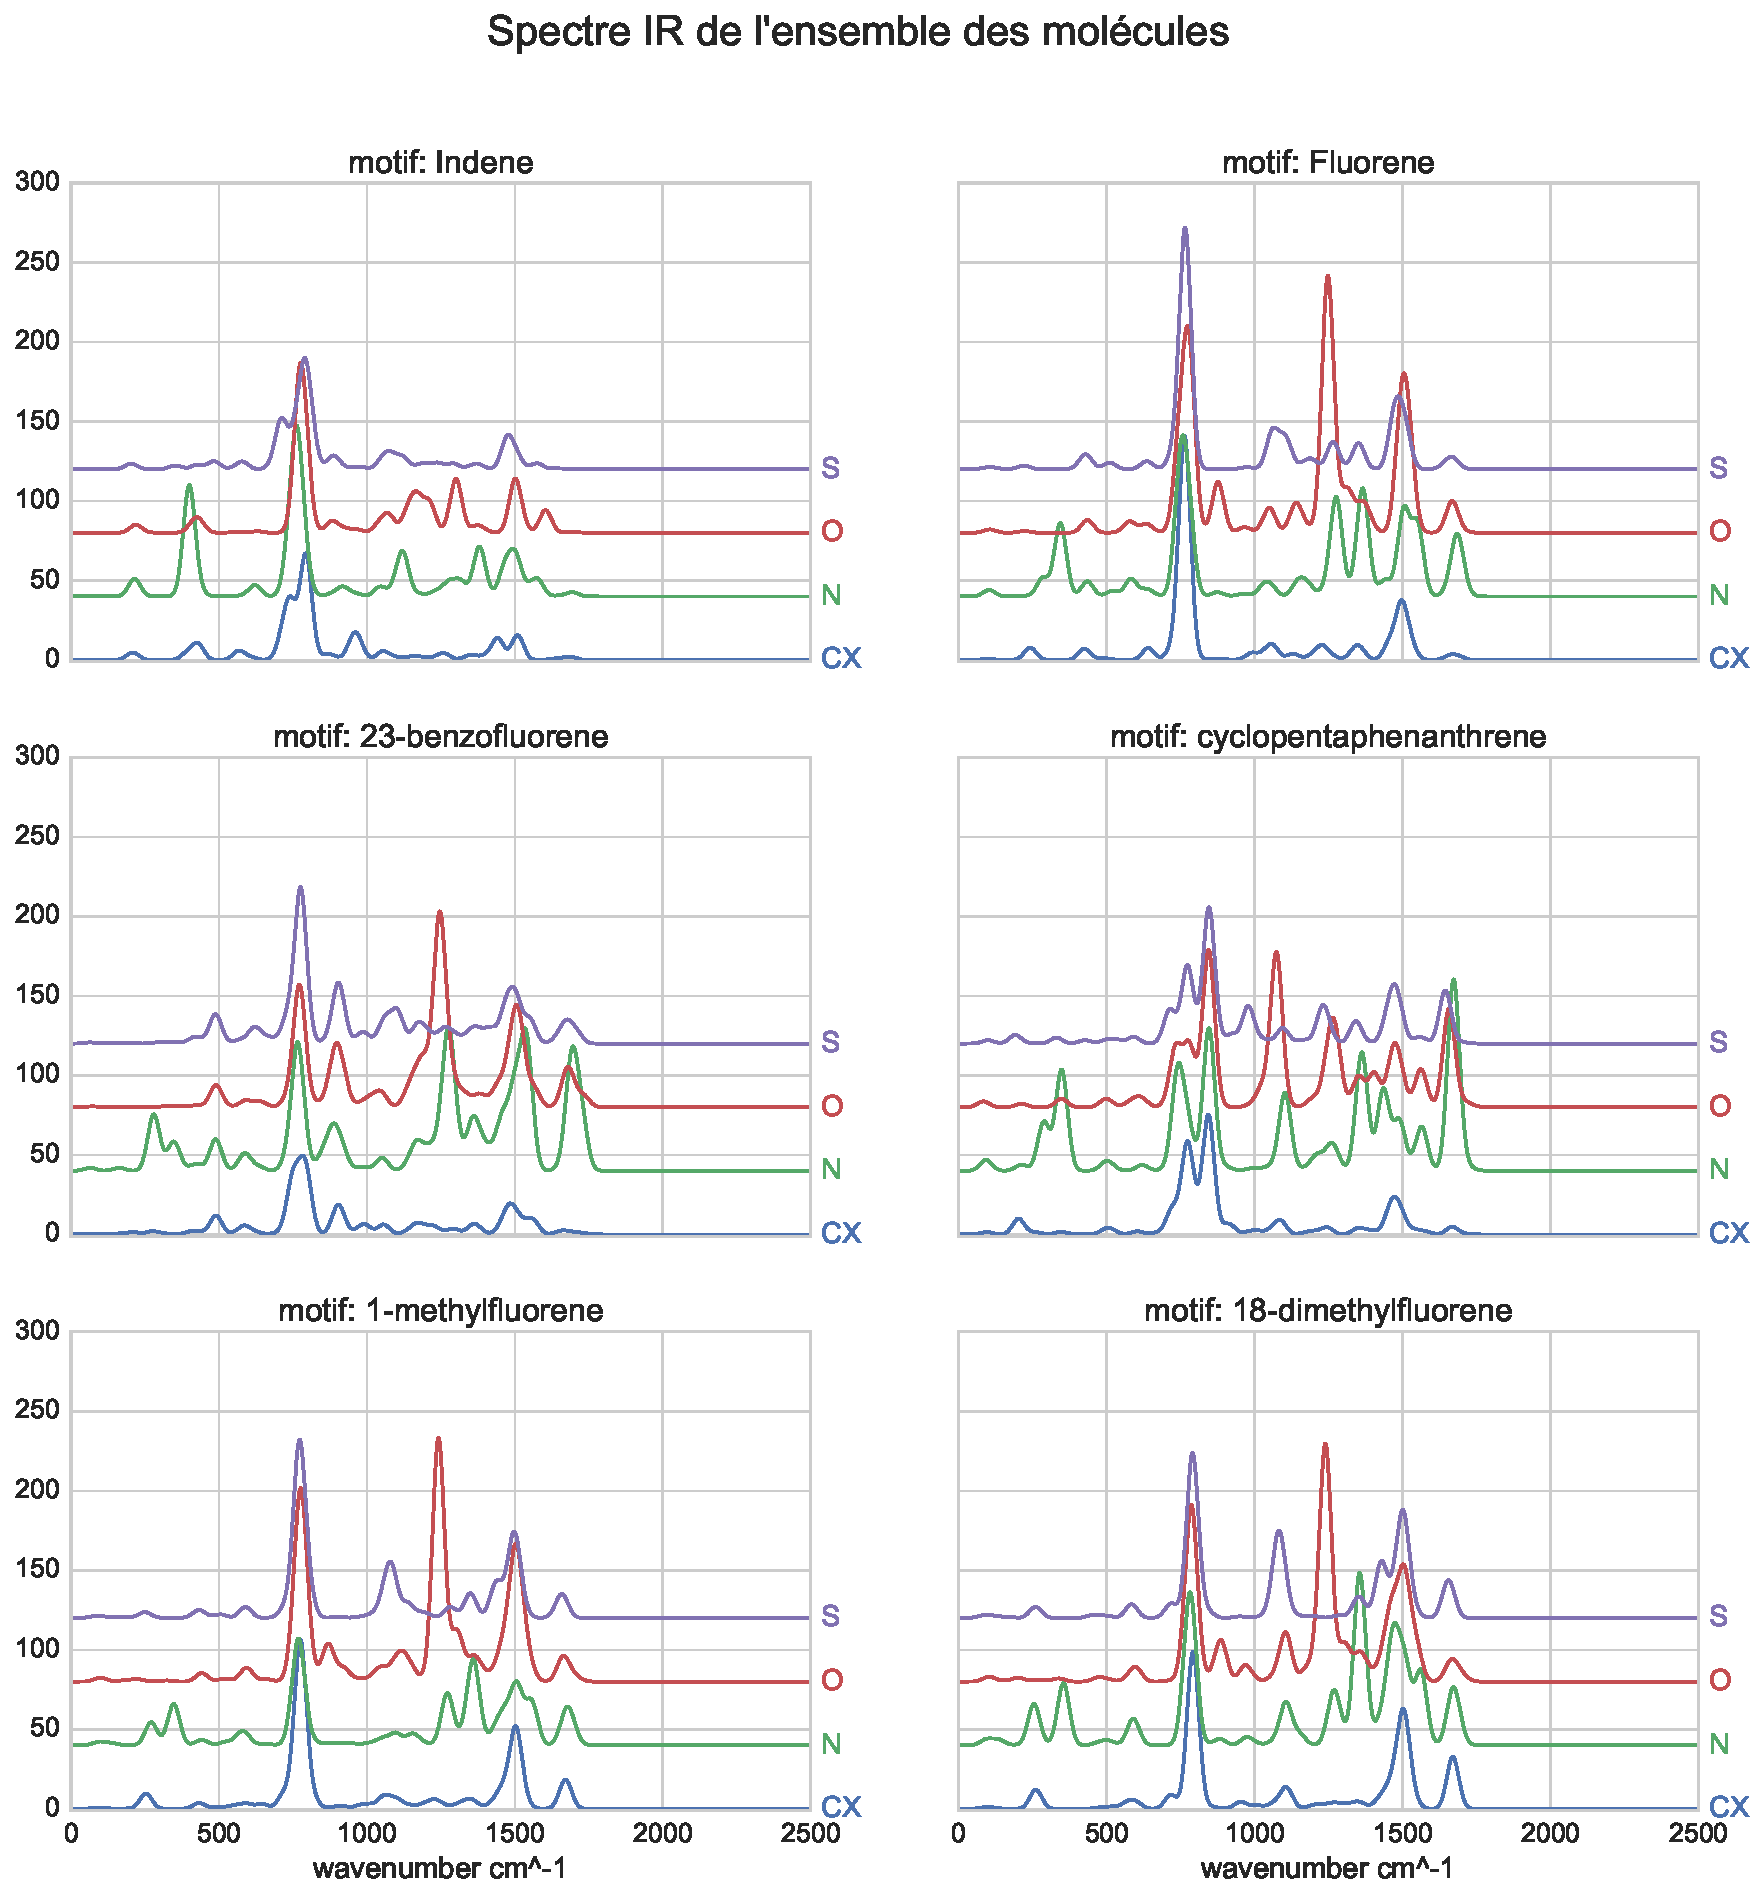
\includegraphics[scale=0.46]{image/P2-4}
		\end{center}
		\caption{Calculated vibrational spectra for all molecules, motifs and heteroatoms comparisons. }  \label{figP2-4}
	\end{figure}
	
Another information concerns now the thiophene family of molecule. If in figure \ref{figP2-2} and \ref{figP2-3} one could verify a non-negligible translation of contributing modes towards the low-wavenumber zone, figure \ref{figP2-4} shows that, in the 700-1600 cm$^{-1}$ (sparsely populated, though) the activity of the remaining modes have not (or very little) lowered in comparison to the equivalent signatures observed for the other hetero atoms (for those, there are no sparsely populated region). The reason behind it is very simple: the majority of the remaining modes imply vibrations of the carbonic backbone that are not very dependant on the hetero atom and are common to all moieties. In this way, it is clear that this spectral zone is of no (or a little) interest to discriminate the spectral behaviours of the different systems. The $x_3=3$ zone is also not very well suited to the discrimination of the vibrators, since it concentrates the most active modes (common to all systems) which the amplitude of the signals can hide all the other signatures. Finally, zones $x_3=1$ and $2$ seem to be more adapted to this discrimination. A finer analysis, mode per mode of these two spectral zones is still necessary in order to identify the singularities of each moiety and each hetero atom, what is reported hereafter.

\subsection{Analyse}

At this point, we should remember that such analysis has a sense only if one tries to product a global information of the spectral behaviour of the molecules (or moieties) potentially present in asphaltenes and, particularly, the signatures of \textit{inter}-molecular signatures on the basis of the samples of chosen model molecules. Of course, if we had the exact formulation of the molecules present in the asphaltenic medium available, it would suffice to model the spectrum of each molecule, for every single moiety and every single heteroatom in order to find, for each molecule, one or several singular characteristics able to discriminate it among the others. Employing mathematical methods dedicated to the resolution of the vibrational Schr\"{o}dinger equation such the ones already presented in chapter 4 (developed within the anharmonic hypothesis) would be enough to provide to spectroscopists useful information (fundamental bands, combination bands, overtones, medium and near IR, Raman, …) The full description of the 24 molecules studied in this work can be found in the Appendix of the manuscript.\\  

The afore reported analysis allows one to bring to light the singular behaviours linked to the presence of heteroatoms and the associated molecules. Despite the fact that this analysis is qualitative and does not allow to conclude concerning the role of each factor. A more detailed analysis of the different modes implicated in each molecule was then necessary to address this problem. In view of the very specific role that the nitrogen hetero atom seem to play, a first detailed study of the carbazole molecule is presented, for which experimental data is available. This will be followed by a second one performed on the dibenzothiophene molecule for which exhaustive experimental data is also available. We should finish by resuming the ensemble of data for each one of the 24 molecules studied in this work, focusing on the differences observed in the $x_3=1$ and $2$ spectral zones (which were previously identified as the one allowing one to discriminate plus efficiently the role of each moiety and heteroatom on the association process).	

\section{Carbazole}

The molecules of the carbazole family are the ones for which the heteroatom contribution to the vibrational modes are the strongest. Another particularity of this family is that the most intense contributions can be found in the lower zones of the spectra. The carbazole monomer presented in figure \ref{figP2-5} depicts these observations. 

 \begin{figure}[H]
 	\begin{center}
 		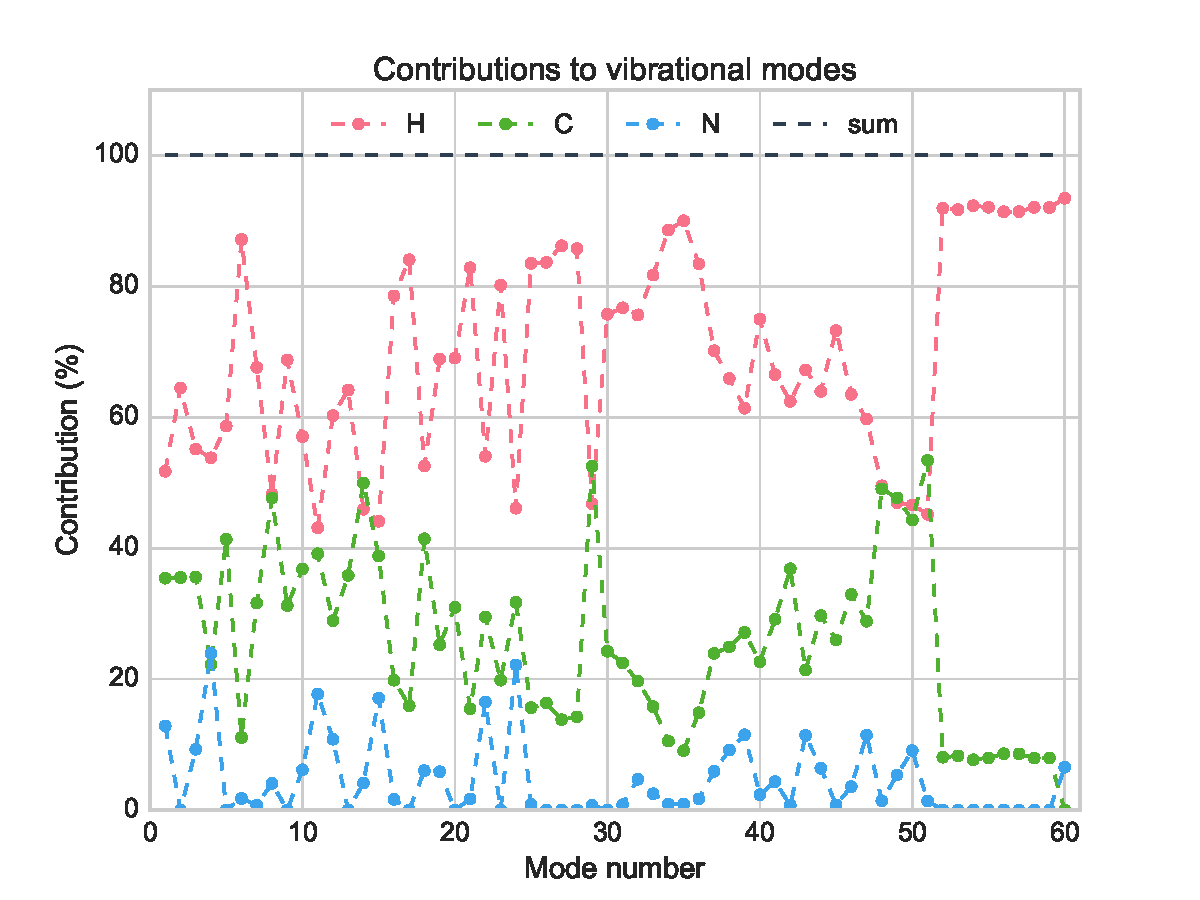
\includegraphics[scale=0.8]{image/P2-5}
 	\end{center}
 	\caption{Atomic percentage contributions to vibrational modes in Carbazole molecule.} \label{figP2-5}
 \end{figure}
	
	
	

	
	Similarly, it becomes clear from this picture that the variations of heteroatom contributions spread over the three spectral zones $x_3=1-3$ and are, exception made to mode 4 ($\omega_{N-H}$), perfectly correlated to the contributions linked to the case where carbon is the heteroatom. These three spectral zones, distributed over around 900 cm$^{-1}$, characterise the ensemble of the signatures of the 25 first modes of carbazole. Among these 25 modes, those for which the contribution of the heteroatom is the most important are repported in figure \ref{figP2-6} by the aforementioned pyctograms. One can note that, except the C-X stretching mode ($\varhexagon$), all the modes depicted by pictograms can be found for carbazole. This information is not enough to allow a rigorous analysis of carbazole’s spectrum. To do so, it is also necessary to take into account at the same time the intensity of each mode and having in hand simultaneously the equivalent information for the dimer molecules if one wishes to characterise the signatures of the \textit{inter}-molecular modes. The ensemble of these pieces of information is reported in Figure \ref{figP2-7}.
	 
	 
	\begin{figure}[H]
		\begin{center}
			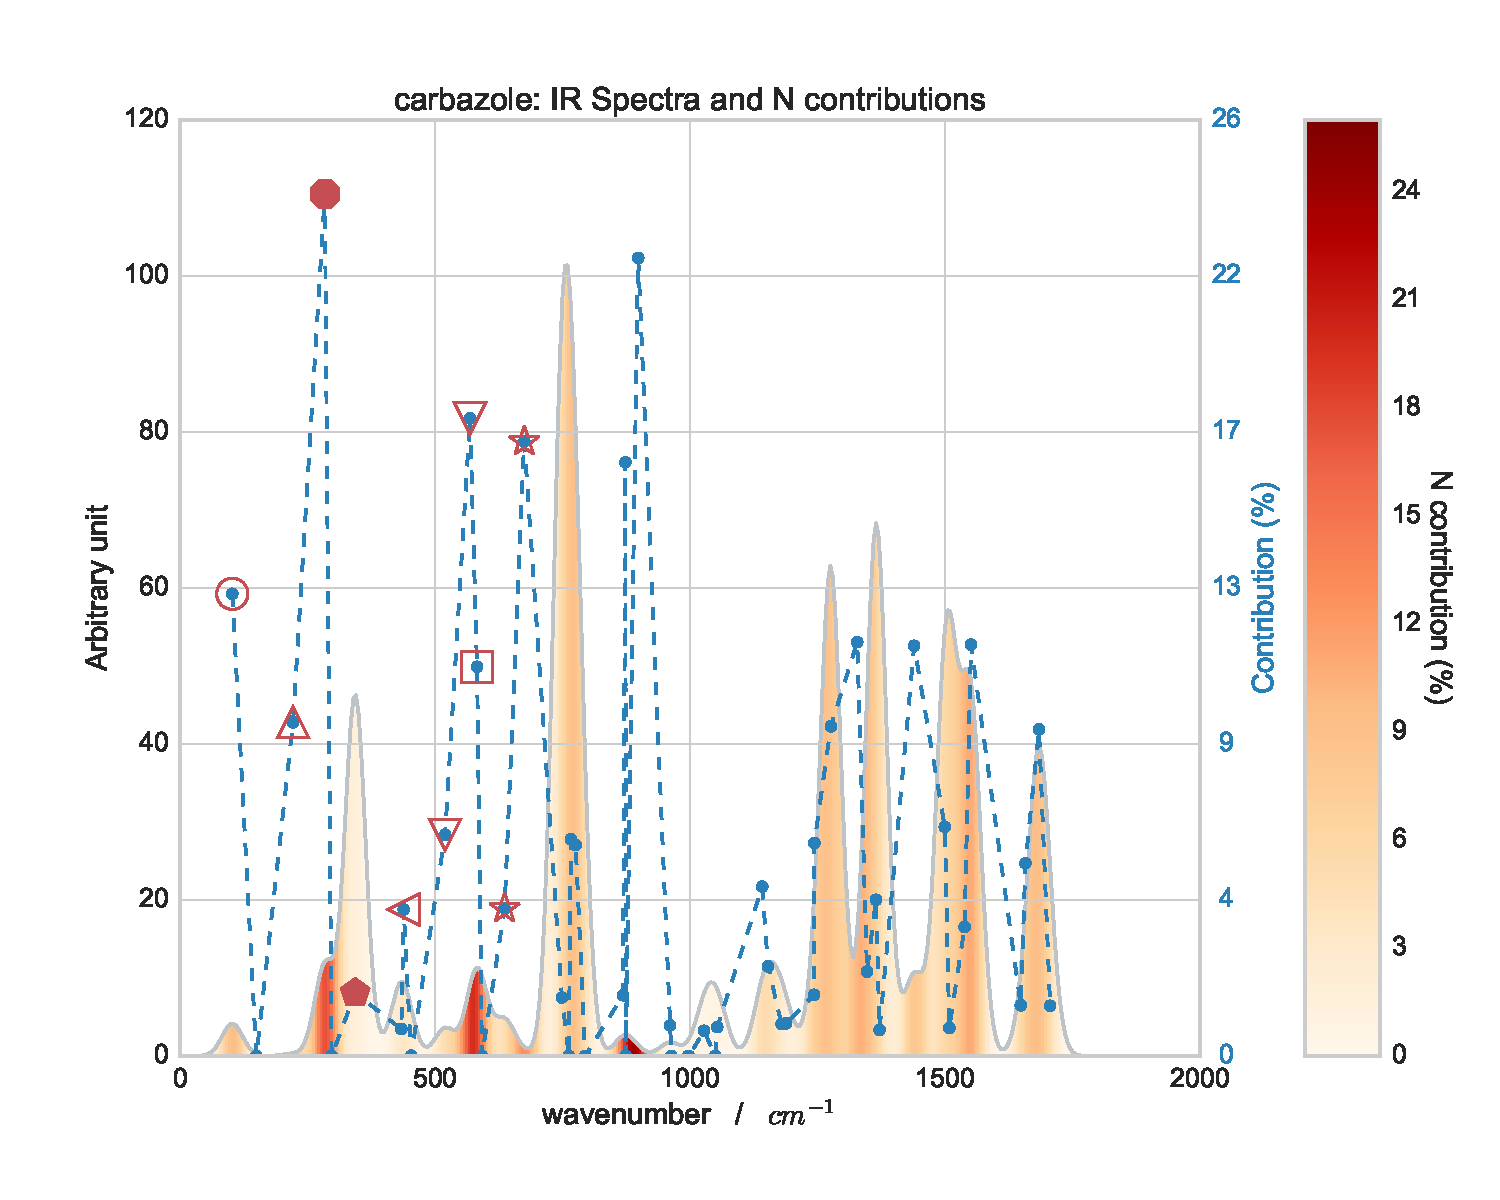
\includegraphics[scale=0.6]{image/P2-6}
		\end{center}
		\caption{Calculated vibrational spectra of Carbazole molecule, showing heteroatom contribution and important modes.}  \label{figP2-6}
	\end{figure}
	

	
	
	The information present in this picture reveals several distinct signs of monomeric and associated carbazole. 1 – a first category of modes seems to distinguish themselves from the others, i.e., those which have a strong contribution of the hetero atom and a strong intensity at the same time. For instance, carbazole’s first modes to own the two characteristics are the twist ($\triangledown$) and wagging ($\square$) ones, found between 550 and 600 cm$^{-1}$. Even if the response of these modes seems to be the most accessible of a spectroscopic point of view, we also could realise that these characteristics are also identically present for the simulations of carbazole dimers. Because of these strong similarities, these modes are thus not useful to our analysis. 2- the presence of \textit{inter}-molecular modes is, on the other hand, more useful. This has been brought to light by our calculations based on the appearing of low intensity signatures at very low wavenumbers which positioning, at least apparently, agrees well with the experimental data reported by K. Michaelin and J. Shaw (figure \ref{figP2-8}). We shall present in this chapter only the results of these specific modes. The quantical treatment of these \textit{inter}-molecular modes will be the subject of development in chapter 6 of this work. However, we should note that these modes are particularly coupled with the others of the deformation type, such as the “butterfly” mode ($\ocircle$). 
	 Consequently, these couplings induce the presence of distinctive differences between the signatures of the monomers and of the dimers within the region nearby the one associated to the \textit{inter}-molecular modes, as it is depicted in Figure \ref{figP2-8}. This is then a zone of interest to us that shall need a very precise description when we will model the vibrational signatures of the systems at the solid state (chapter 6).
	 
	 
	 	\begin{figure}[H]
	 		\begin{center}
	 			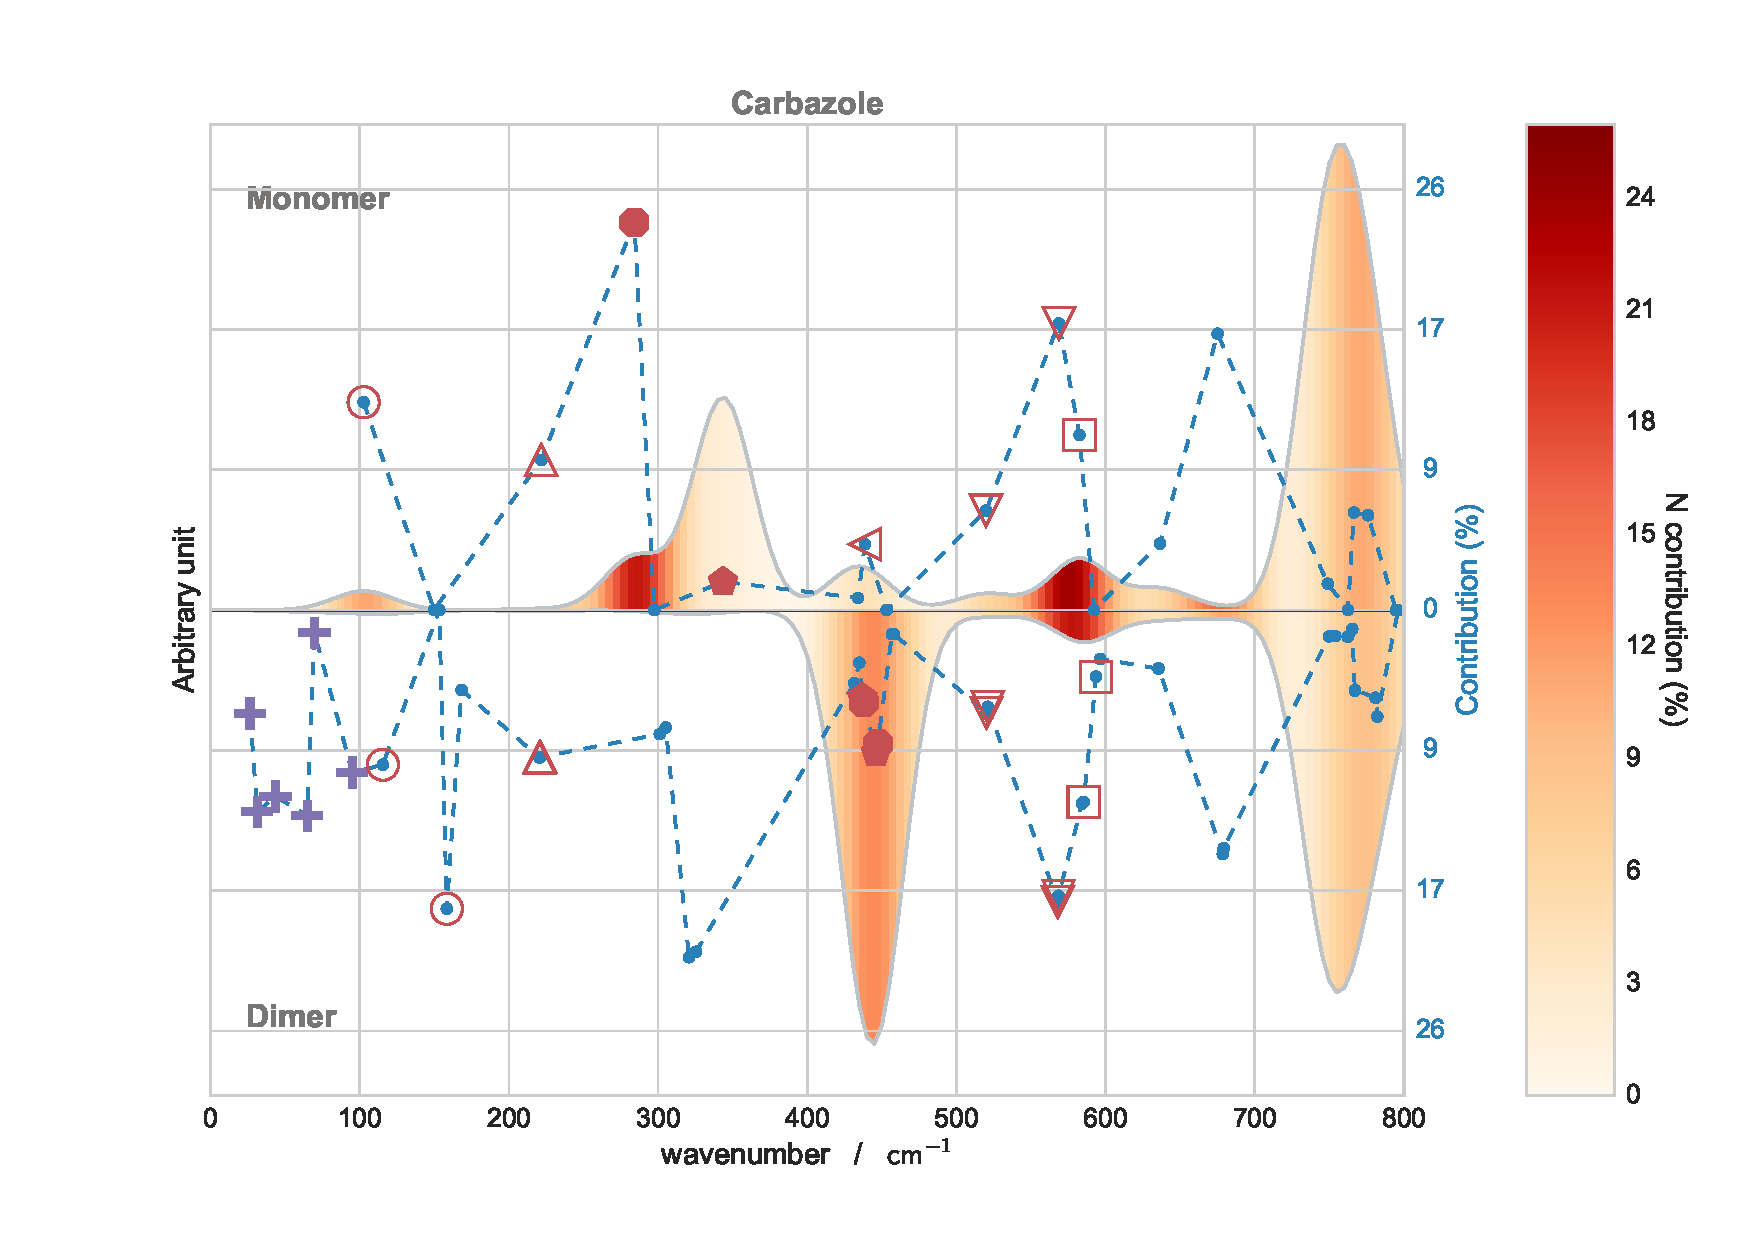
\includegraphics[scale=0.5]{image/P2-7}
	 		\end{center}
	 		\caption{Calculated vibrational spectra of Carbazole monomer and dimer, between 0- 800 cm$^{-1}$, showing heteroatom contribution and important modes.}  \label{figP2-7}
	 	\end{figure}
	 	
	 		\begin{figure}[H]
	 			\begin{center}
	 				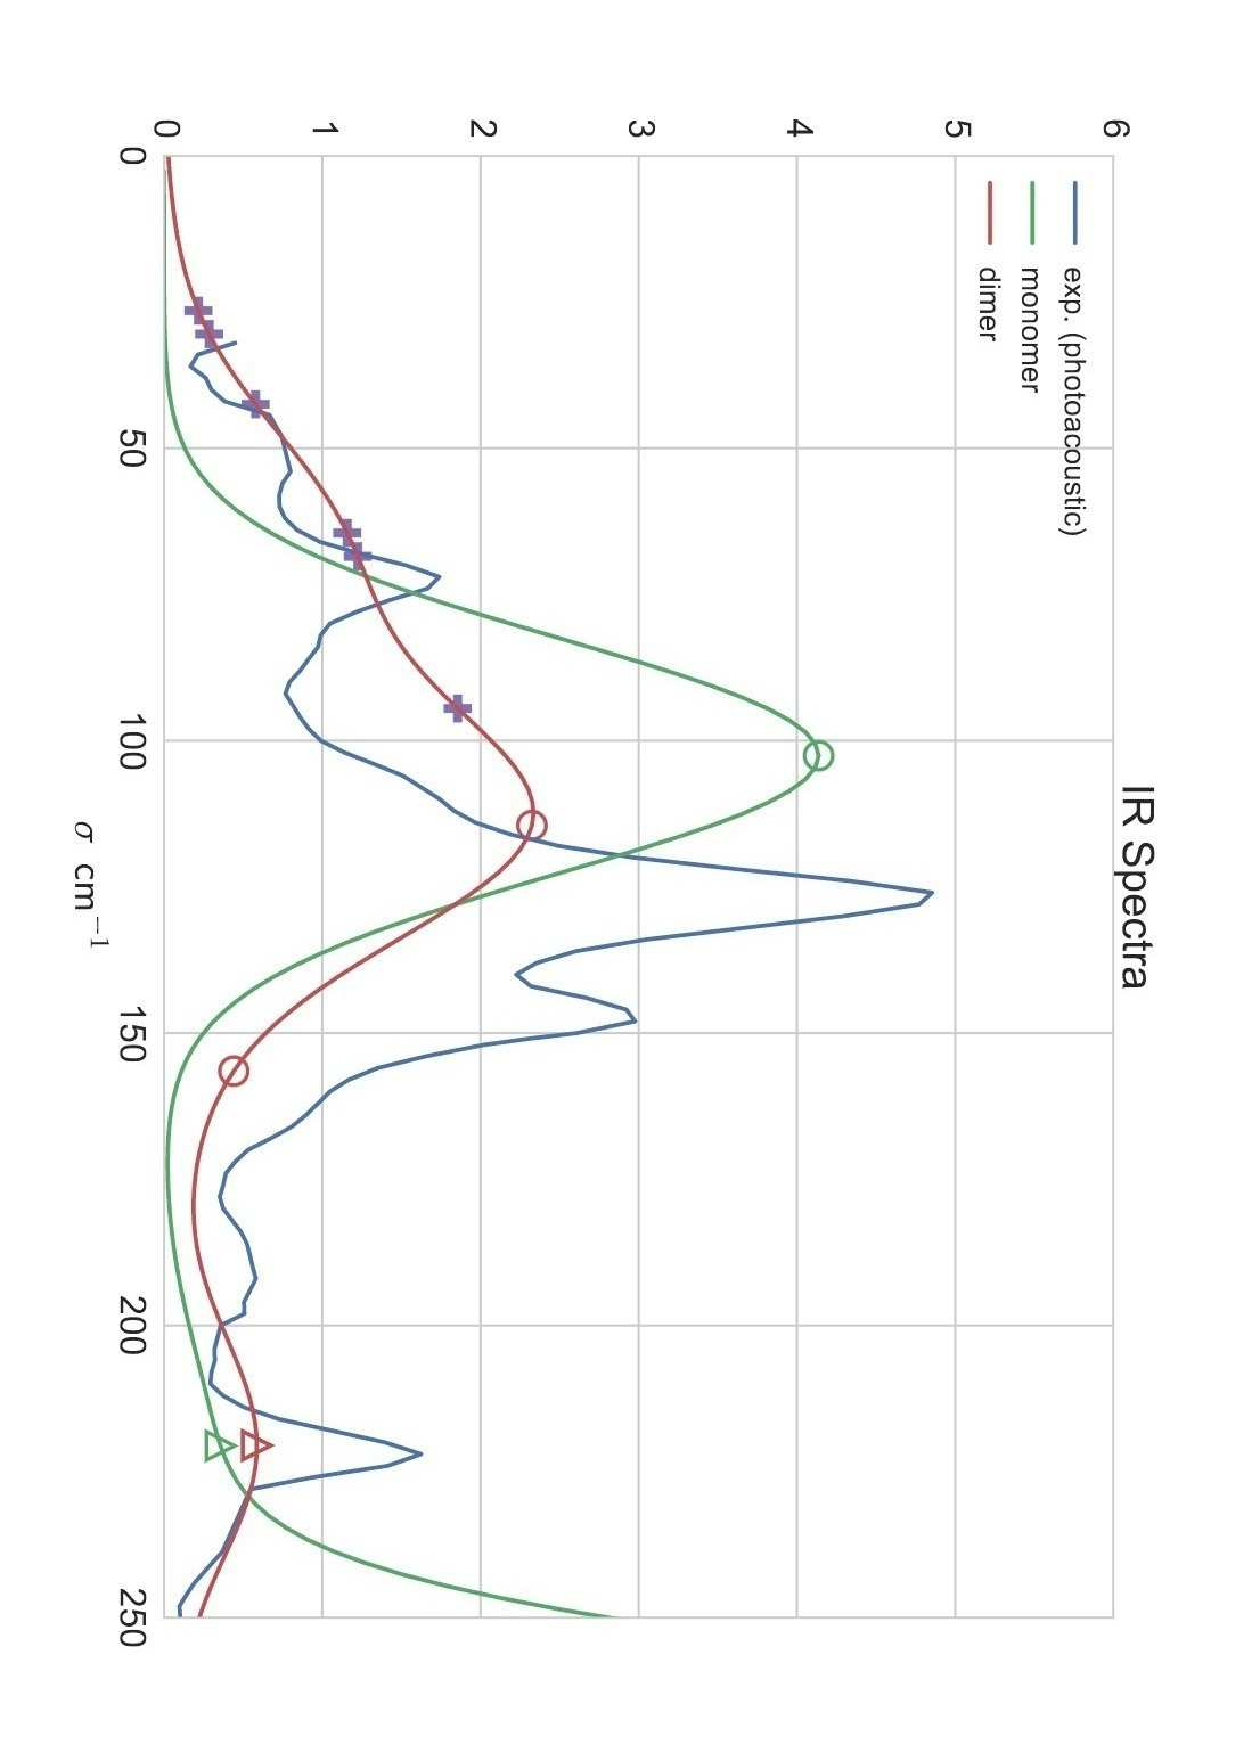
\includegraphics[angle=90,scale=0.32]{image/8}
	 			\end{center}
	 			\caption{Comparison between calculated vibrational spectra of monomer and dimer with IR experimental at 0- 250 cm$^{-1}$ of Carbazole} \label{figP2-8}
	 		\end{figure}
	 		
	 		
	
	Another category of modes that are specific to the carbazole family will allow us to highlight the presence of moieties associated as shown by the experiments conducted by K. Michaelian. So that the characterisation of these specific modes can be done, we have reported in figure 9 the evolution of the density of vibrational states against the vibrational frequencies for carbazole’s monomer and dimer. It appears distinctly in figure \ref{figP2-9} two zones with strong densities within the zone $x_3=2$ (comprised between 250-500 cm$^{-1}$) that should indicate strictly the presence of two spectral zones in the experimental spectrum. Yet, one can found in this spectrum only intense zone centered at 450 cm$^{-1}$. Nevertheless, a very weak activity is noted around 300 cm$^{-1}$, precisely at the same place where there is a strong density of vibrational states. 
	
	\begin{figure}[H]
		\begin{center}
			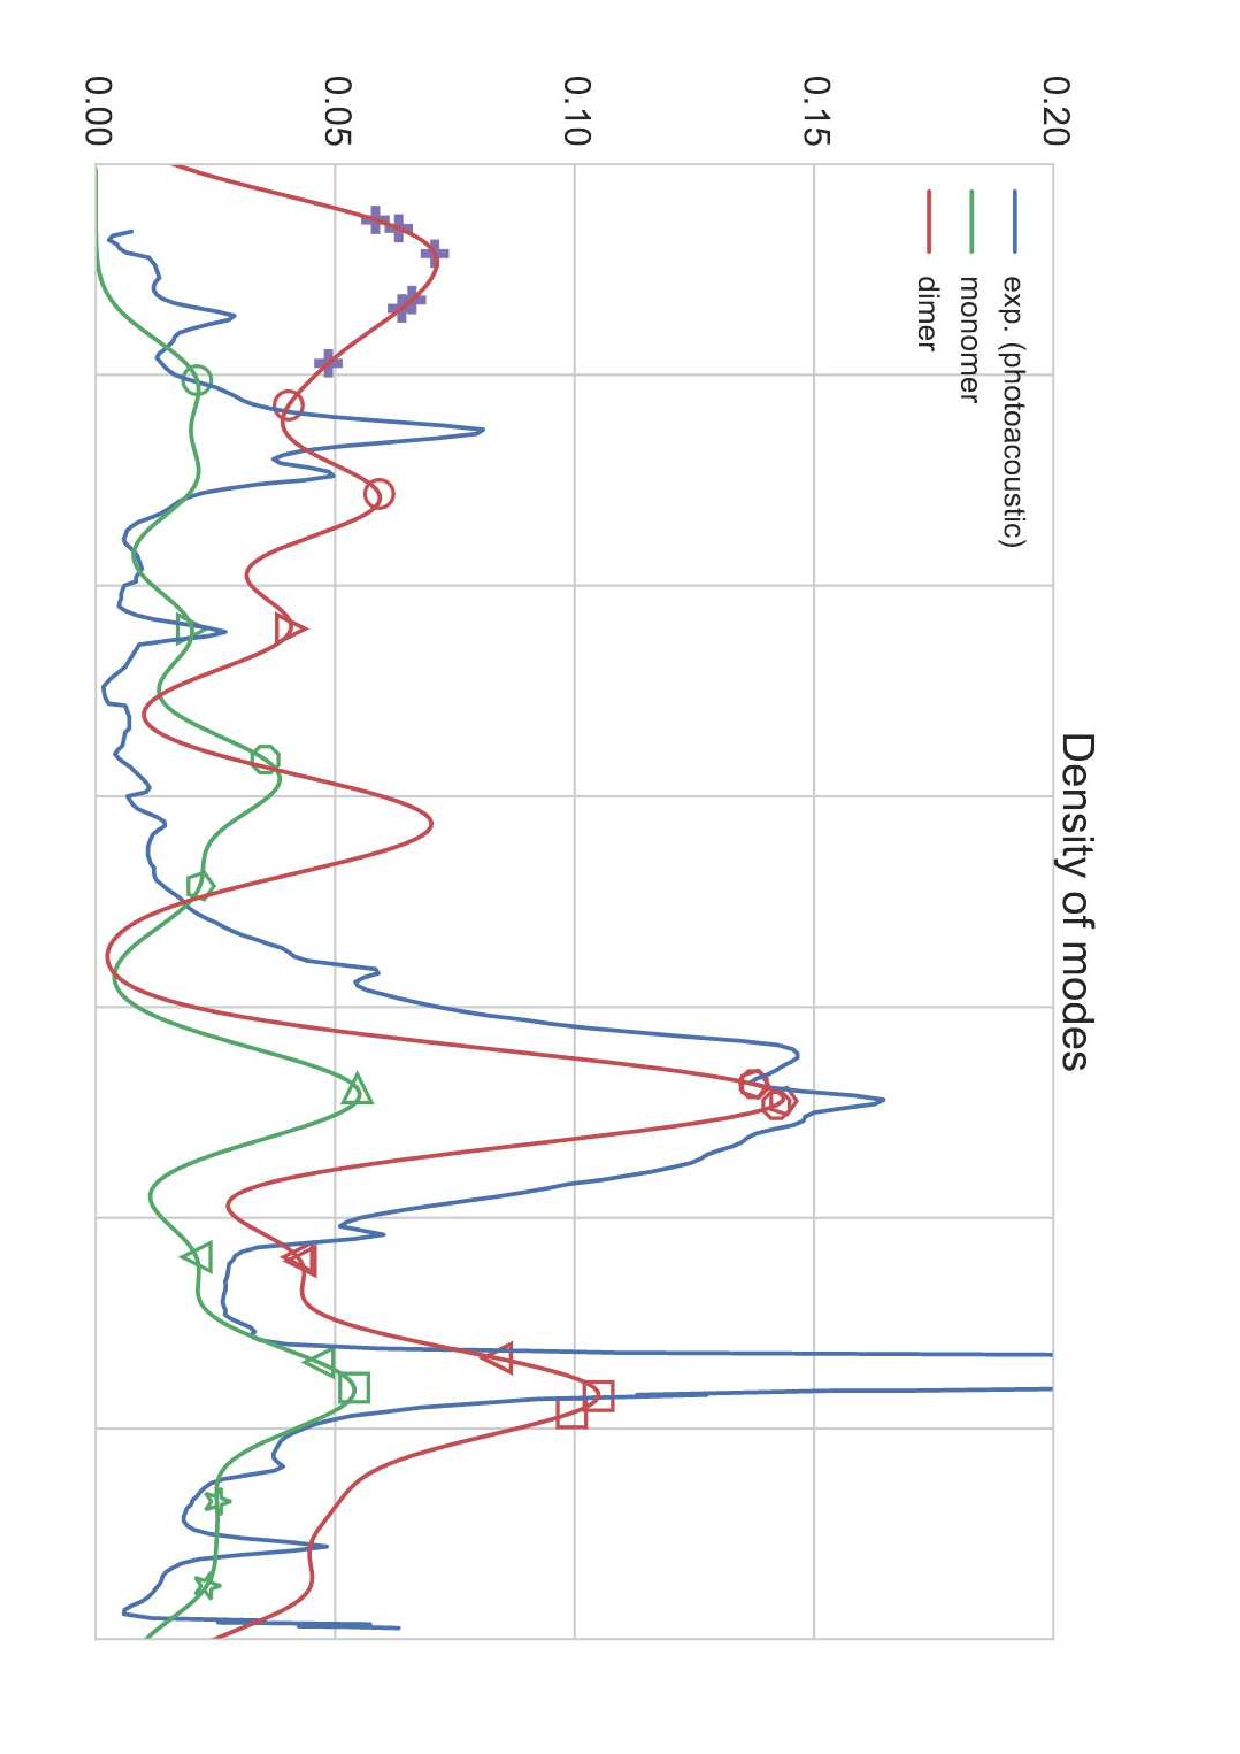
\includegraphics[angle=90,scale=0.5]{image/9}
		\end{center}
		\caption{Comparison of density of modes at low wavenumber region of Carbazole.}  \label{figP2-9}
	\end{figure}
	
	
	Our calculations also show that all the dimer’s modes (however more numerous than those of the monomers in this zone) present around 300 cm$^{-1}$ are practically all inactive. On the other side, if the density of modes for the monomer in this region is weaker than the one of the dimer, the 280-300 cm$^{-1}$ zone remains potentially the place where detectable signatures could be found for this specie (as it is depicted in figure \ref{figP2-7}). The analysis of a second regions centred at 450 cm$^{-1}$ reveals this time that two species (monomer and dimer) have both of them a stronger density of modes, but oppositely to the dimer, no monomer’s vibration mode localised within this region have a strong signature. Another very important information concerns the N-H wagging modes ($\pentagon$ and $\octagon$)
	  at the origin of monomer’s spectral signature in the 280-350 cm$^{-1}$ zone. As a result of the presence of \textit{inter}-molecular interactions, the position of these modes is strongly displaced towards higher wavenumbers for the dimer. Surprisingly, they are displaced to around 450 cm$^{-1}$, what induces an augmentation of the dimer’s modes density in this region. Experimentally, this region is where a strong, wide spectral band having several bumps can be found and this seems to agree well with what was calculated for the associated specie (and reported in figure \ref{figP2-10}, on which the modes’ intensities are also shown alongside their densities). Moreover, the 280-350 cm$^{-1}$ zone is here the experimental spectral signatures are weak and this corroborates a little more the fact that carbazole is not present as a monomer (at least not predominantly)  when the spectrum was recorded.
	 
	 	\begin{figure}[H]
	 		\begin{center}
	 			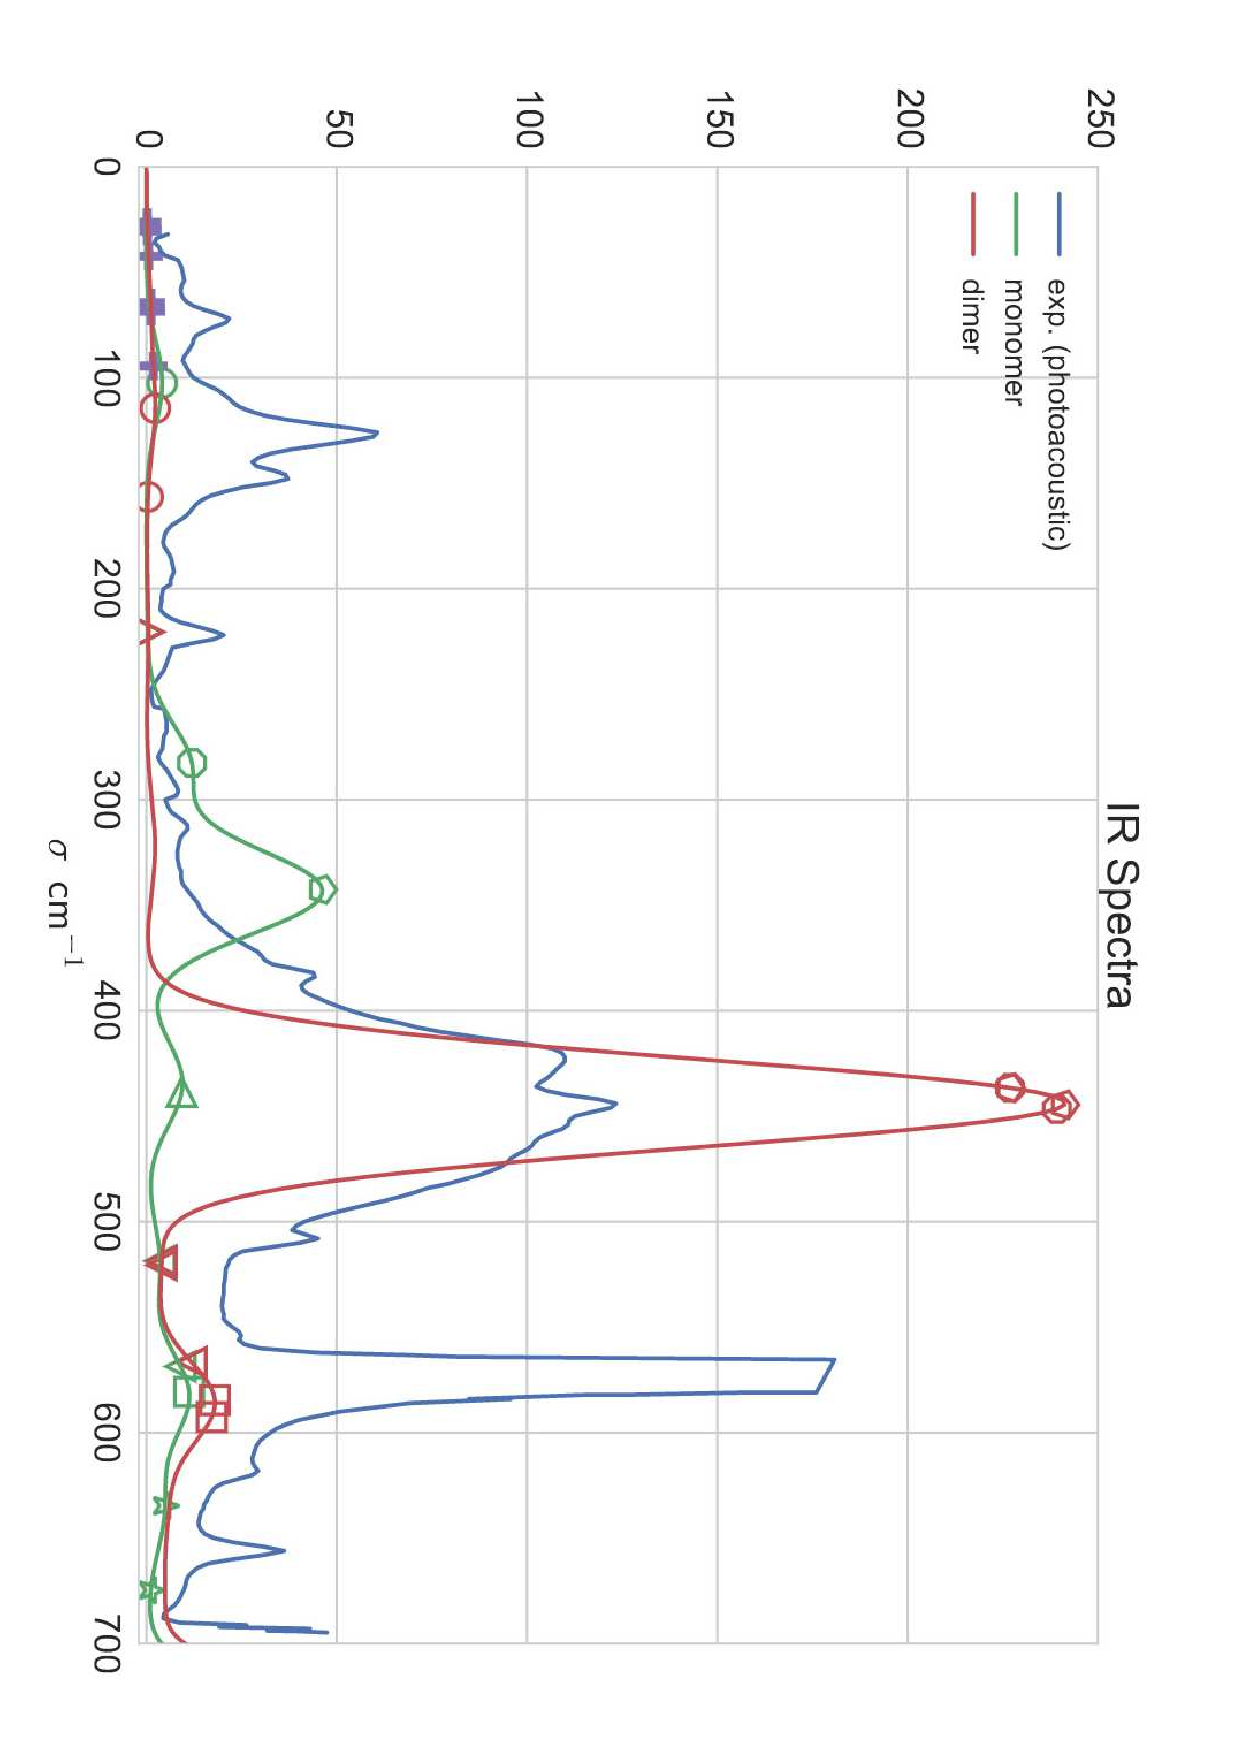
\includegraphics[angle=90,scale=0.5]{image/10}
	 		\end{center}
	 		\caption{Comparison of calculated vibrational spectra and experimental data taking into account theoretical intensities for Carbazole.}  \label{figP2-10}
	 	\end{figure}
	 
	 Given the fact that we do not have experimental data for the other molecules of the carbazole family, we can not verify the validity of our hypothesis for all the species. But we can report the shifts of the N-H wagging modes predicted by our calculations and show that they are not specific to the carbazole system only for the family having nitrogen as the heteroatom (figures \ref{figP2-11ad}). Yet, the spectra reported in figures \ref{figP2-11ad} clearly show that the shifts of the wagging modes signatures are not all equivalent and apparently they strongly depend on the system in question. In figure 1\ref{figP2-12}, the pieces of information concerning these shifts were regrouped aiming to find an explanation concerning the influence of the substituent or the moiety. Unluckily, no direct link connecting the intensity of these shifts and any particular symmetry of these moieties, or the position of the substituent in the molecule, the number of them, etc, for instance, could be found. On the other hand, these results clearly show that these shifts concern only the species of the carbazole family. A deeper study will then be presented in the following paragraphs. 
	
	
	\begin{figure}[H]
		\begin{center}
			\resizebox{17cm}{!}{
			\begin{tabular}{c c}
				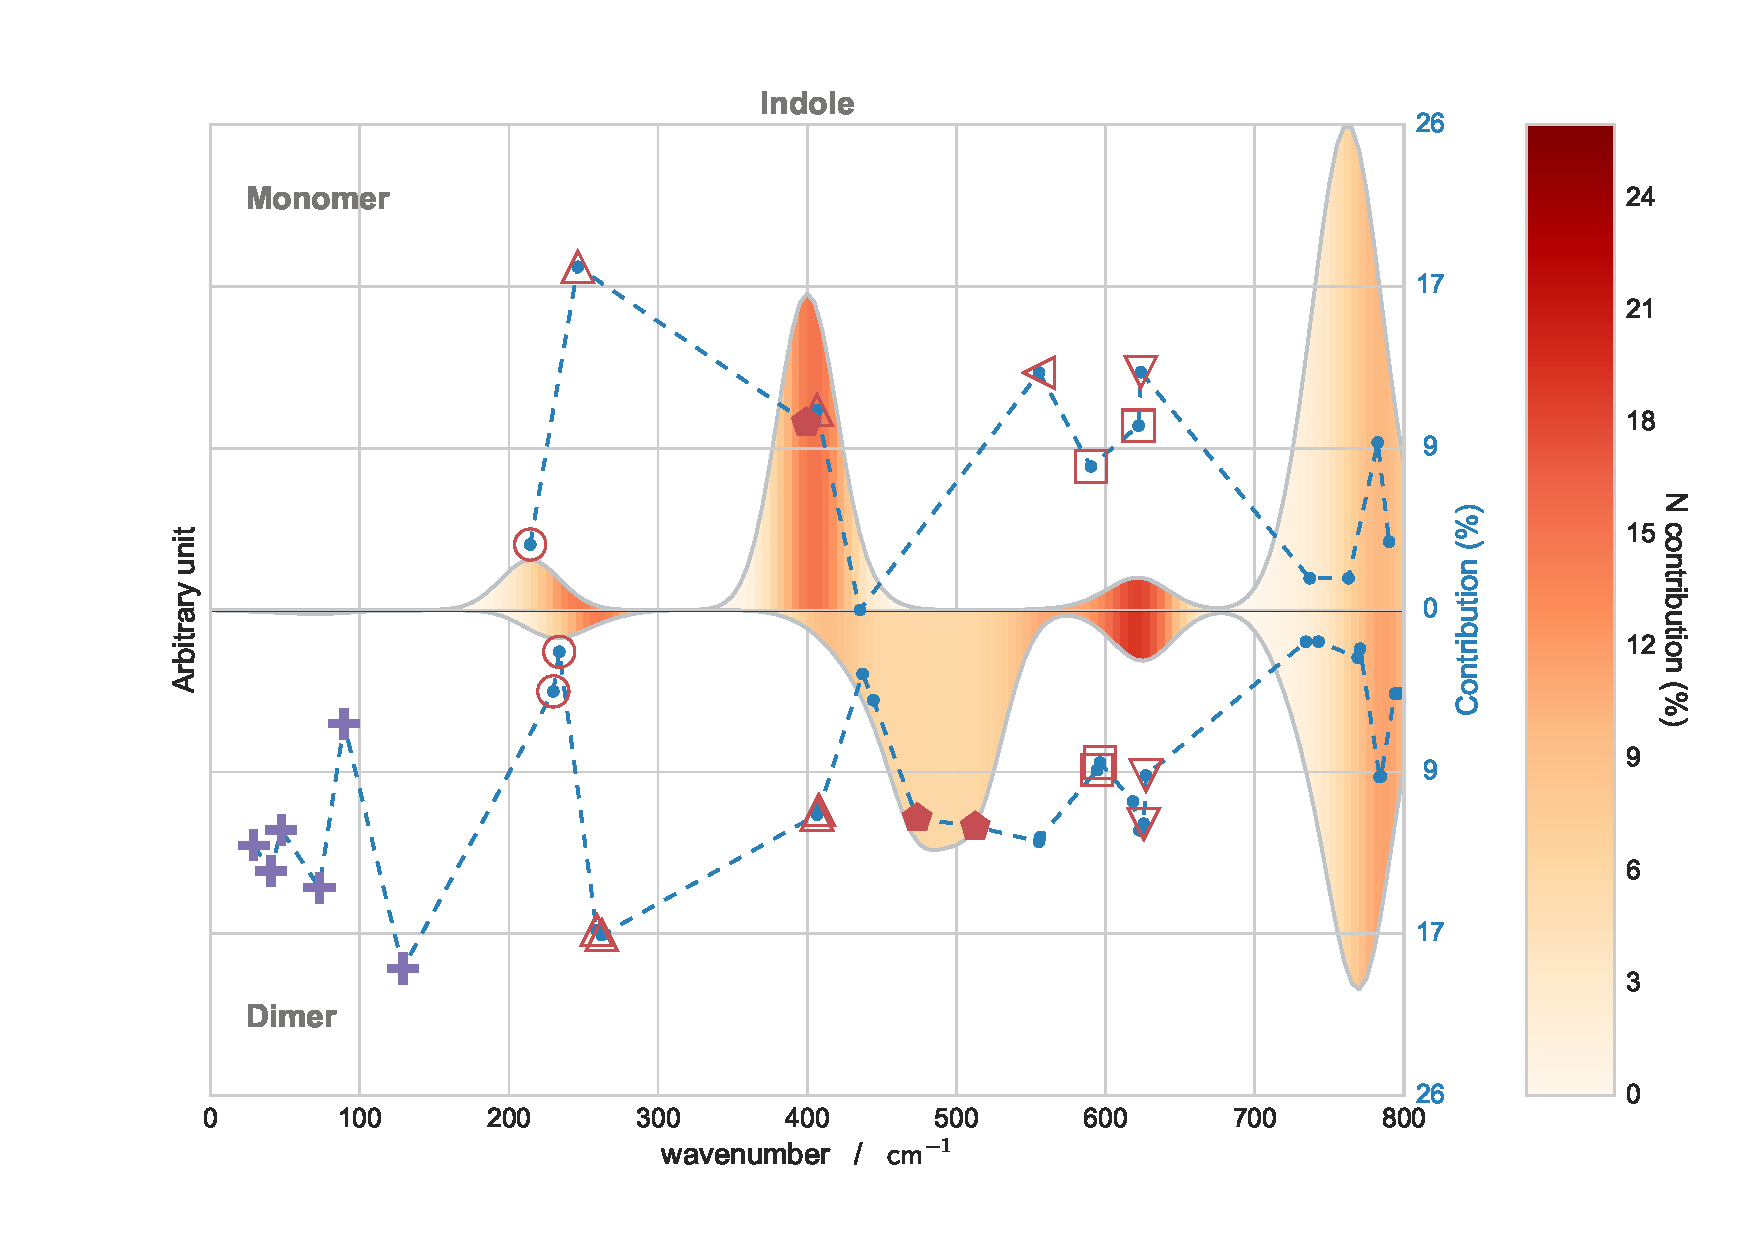
\includegraphics[scale=0.3]{image/P2-11a} & 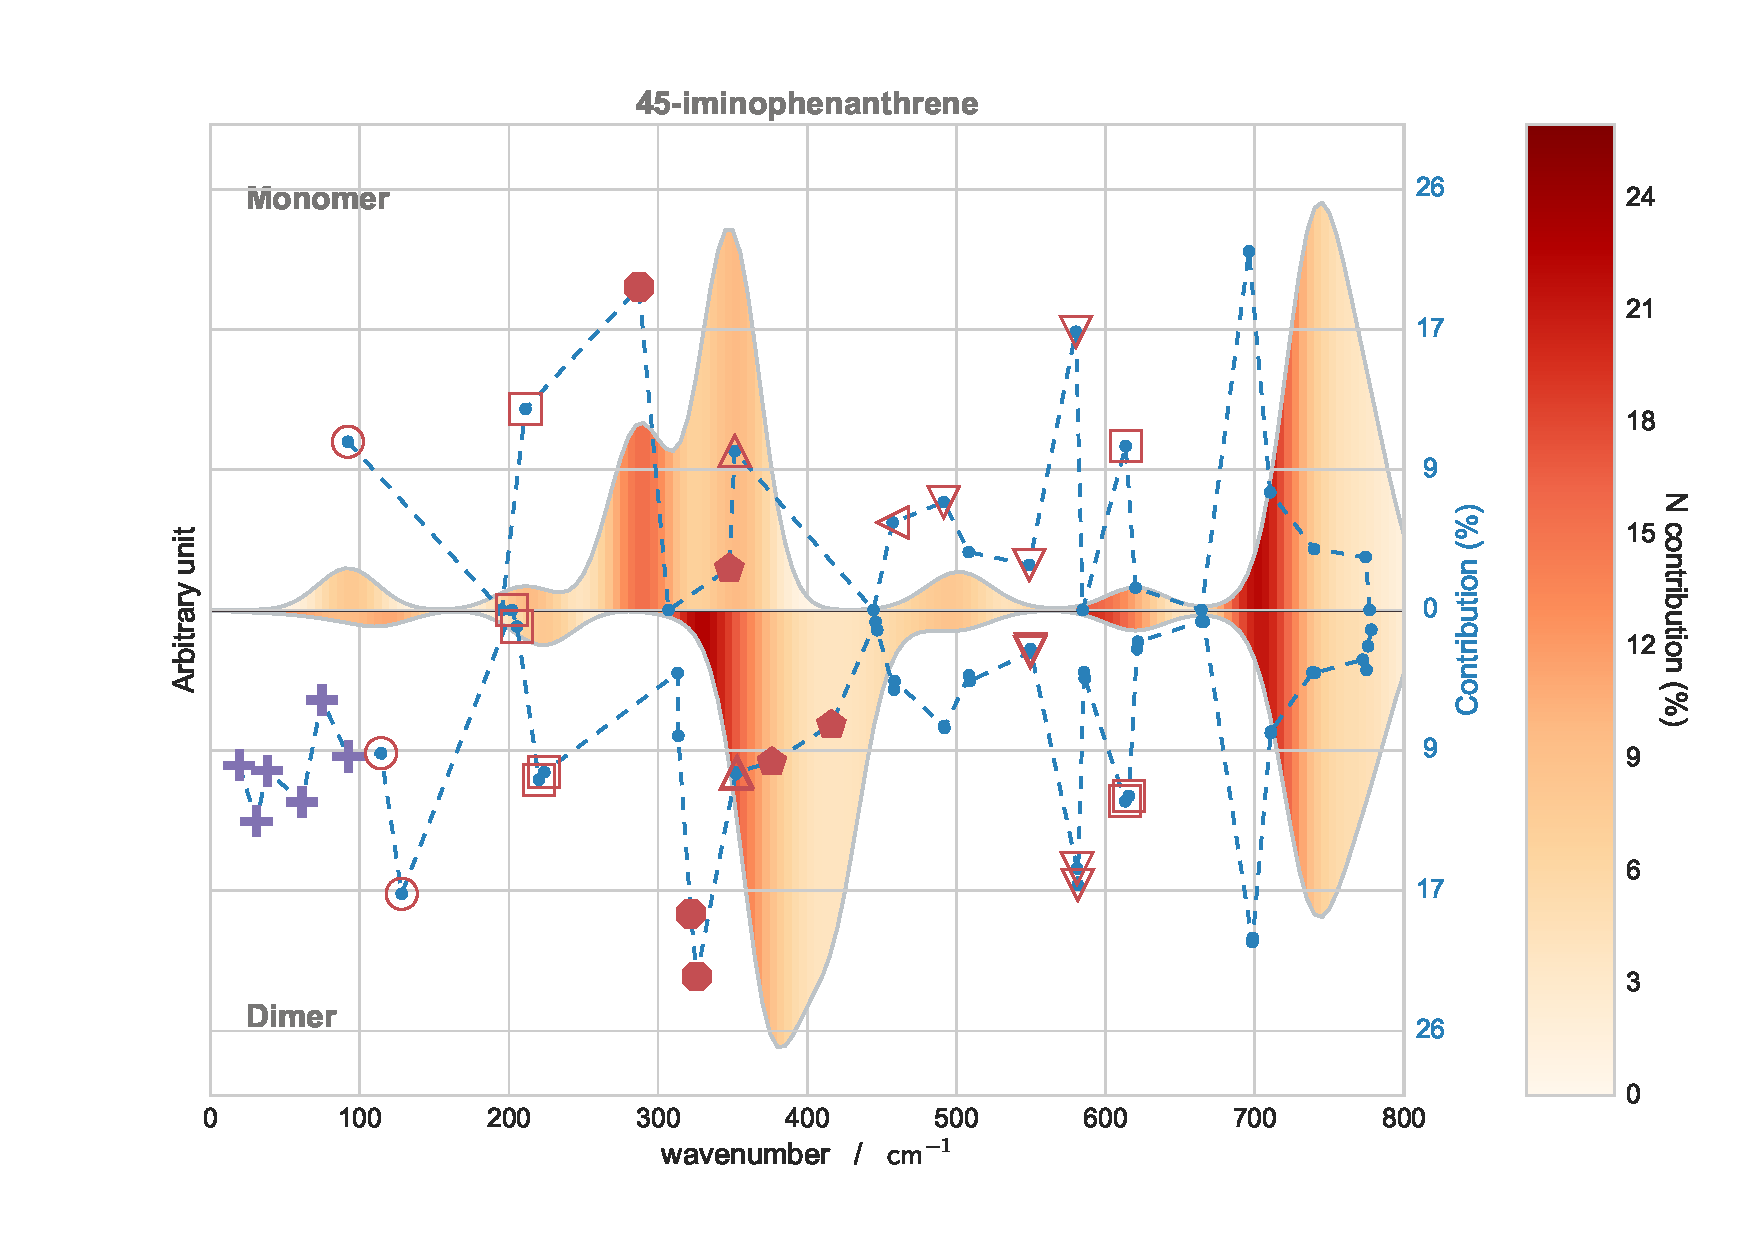
\includegraphics[scale=0.3]{image/P2-11b} \\
				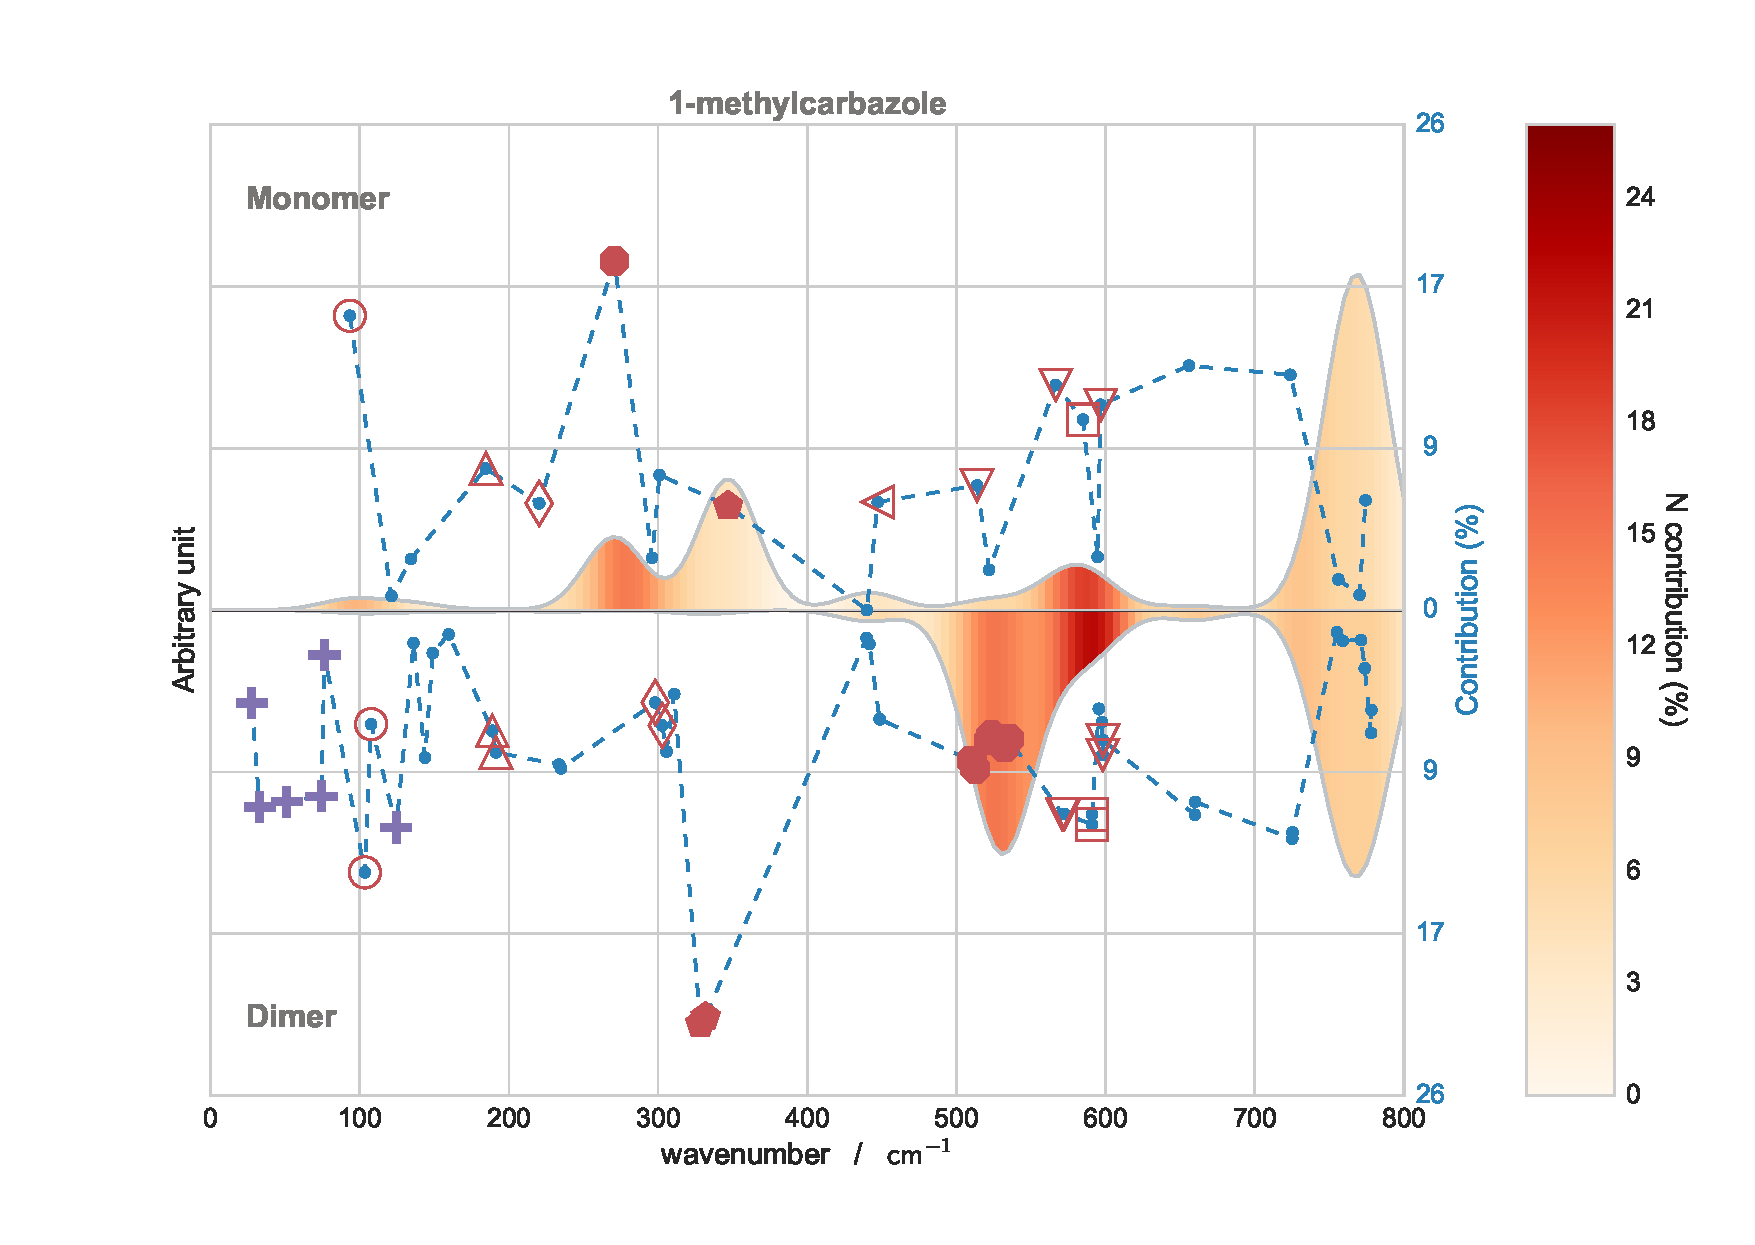
\includegraphics[scale=0.3]{image/P2-11c} & 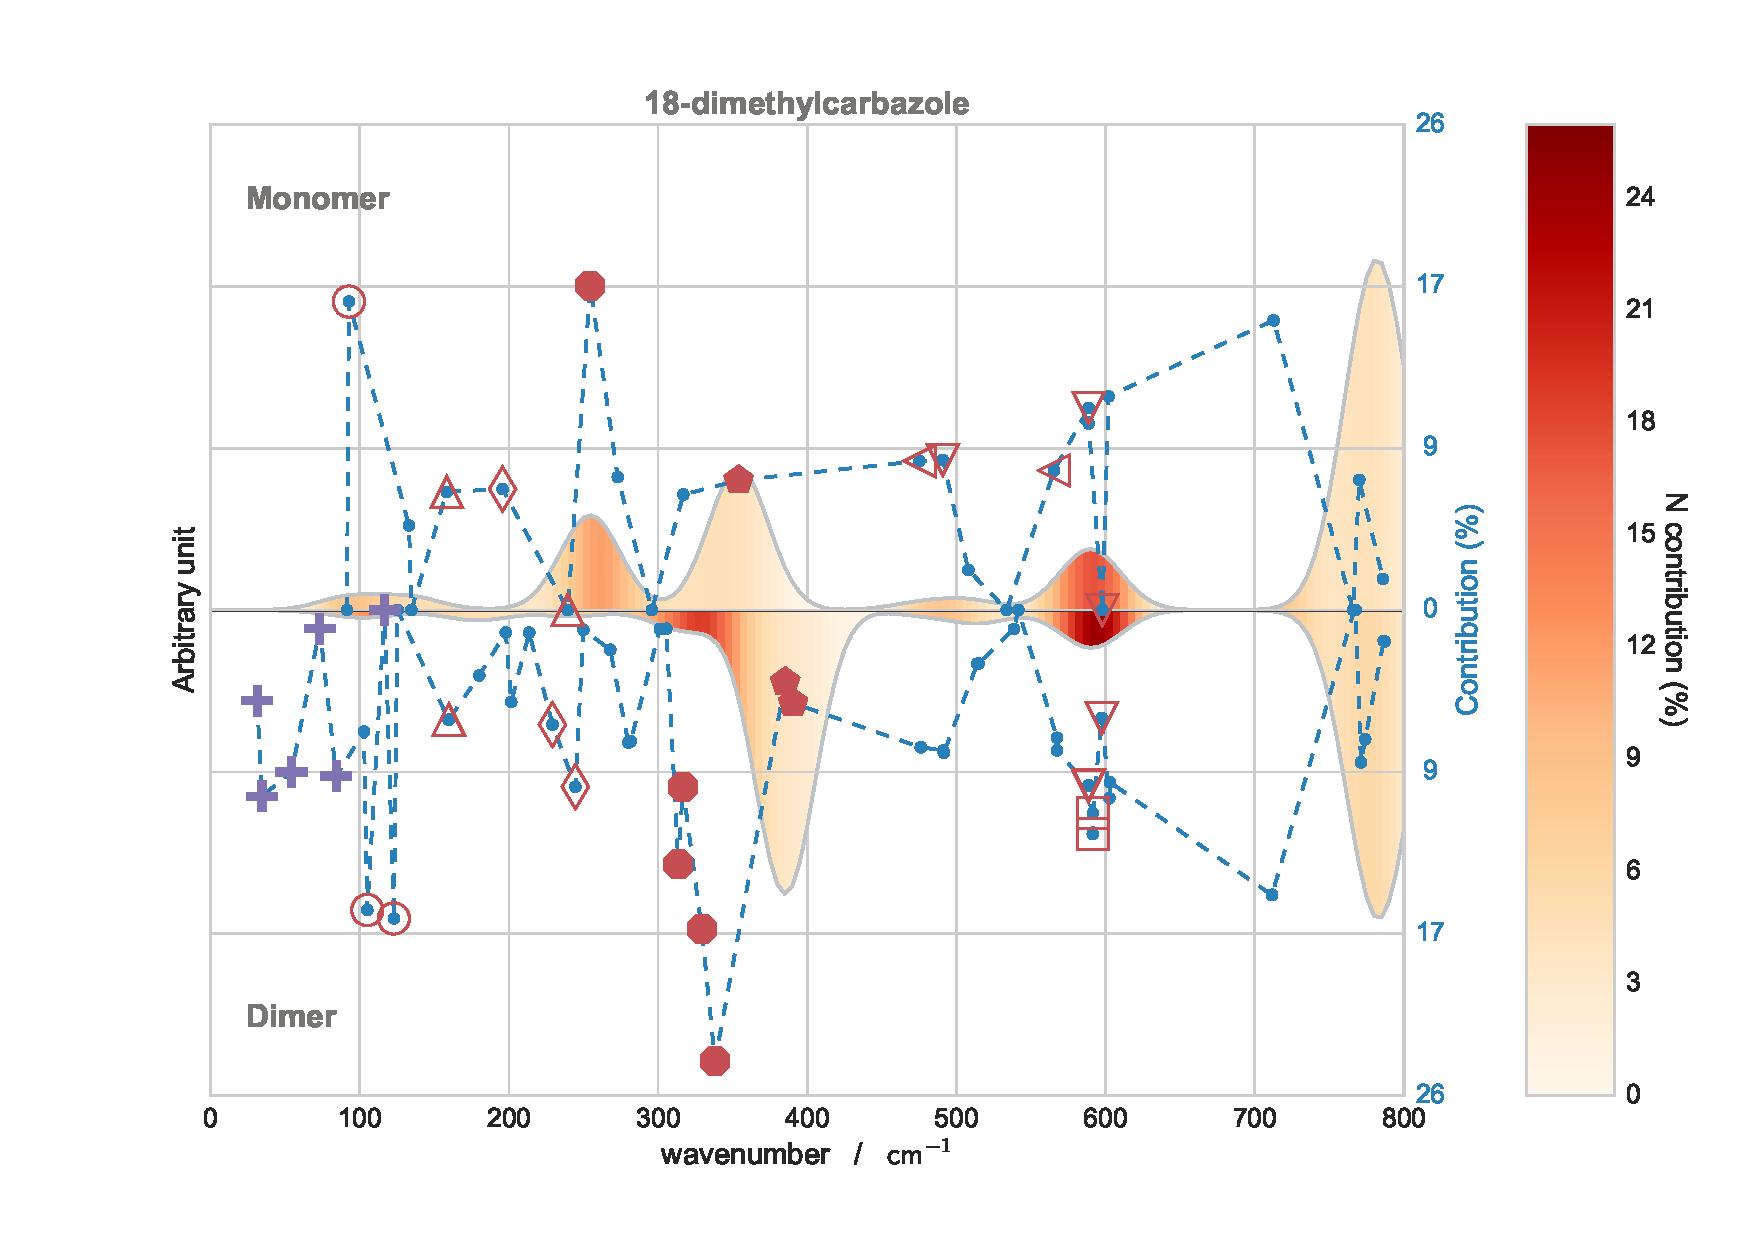
\includegraphics[scale=0.3]{image/P2-11d}\\
		\end{tabular}}
	\end{center}
		\caption{Comparison between momoner and dimer calculated vibrational spectra for \textbf{a} Indole, \textbf{b} 4,5-iminophenanthrene, \textbf{c} 1-methylcarbazole and \textbf{d} 1,8-dimethylcarbazole at 0- 800 cm$^{-1}$ interval.} \label{figP2-11ad}
	\end{figure}
	
	
	\begin{figure}[H]
		\begin{center}
			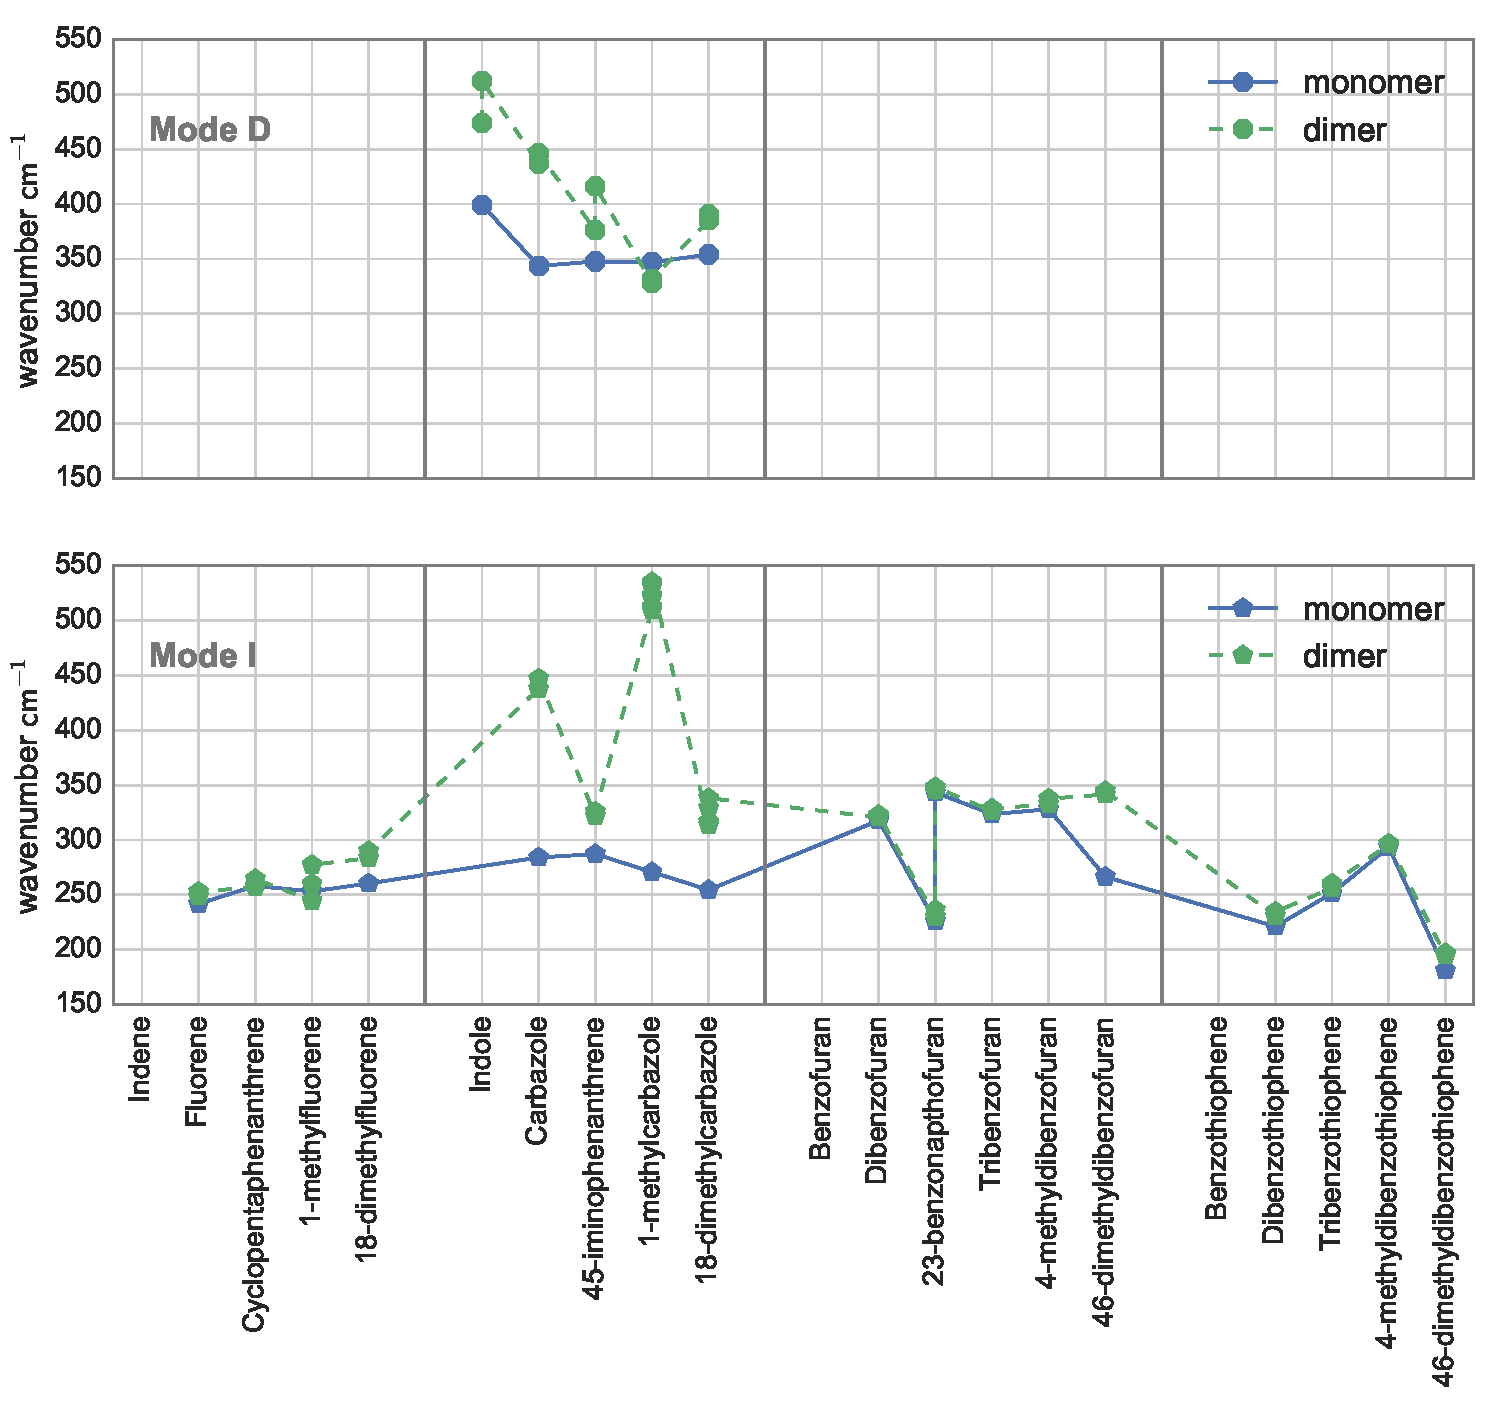
\includegraphics[scale=0.33]{image/P2-12}
		\end{center}
		\caption{Variation of D and I modes between monomer- dimer of studied molecules} \label{figP2-12}
	\end{figure}
	
	
	In summary, two type of modes characteristic to the associated systems bearing nitrogen as the heteroatom were highlighted in our work: they are \textit{inter}-molecular modes localised at very low wavenumbers and N-H wagging modes for which the frequency, \textit{in fine}, strongly depends on the presence or not of \textit{inter}-molecular interactions. 
	
	
	
	\section{Dibenzothiophene}
	
	
	For dibenzothiophene monomer and dimer, their results are very similar for what concerns the frequency, intensity and sulphur contribution to all the vibrations. The only exceptions are the particularities listed for the nitrogen as heteroatom case (N-H wagging).
	
	
	\begin{figure}[H]
		\begin{center}
			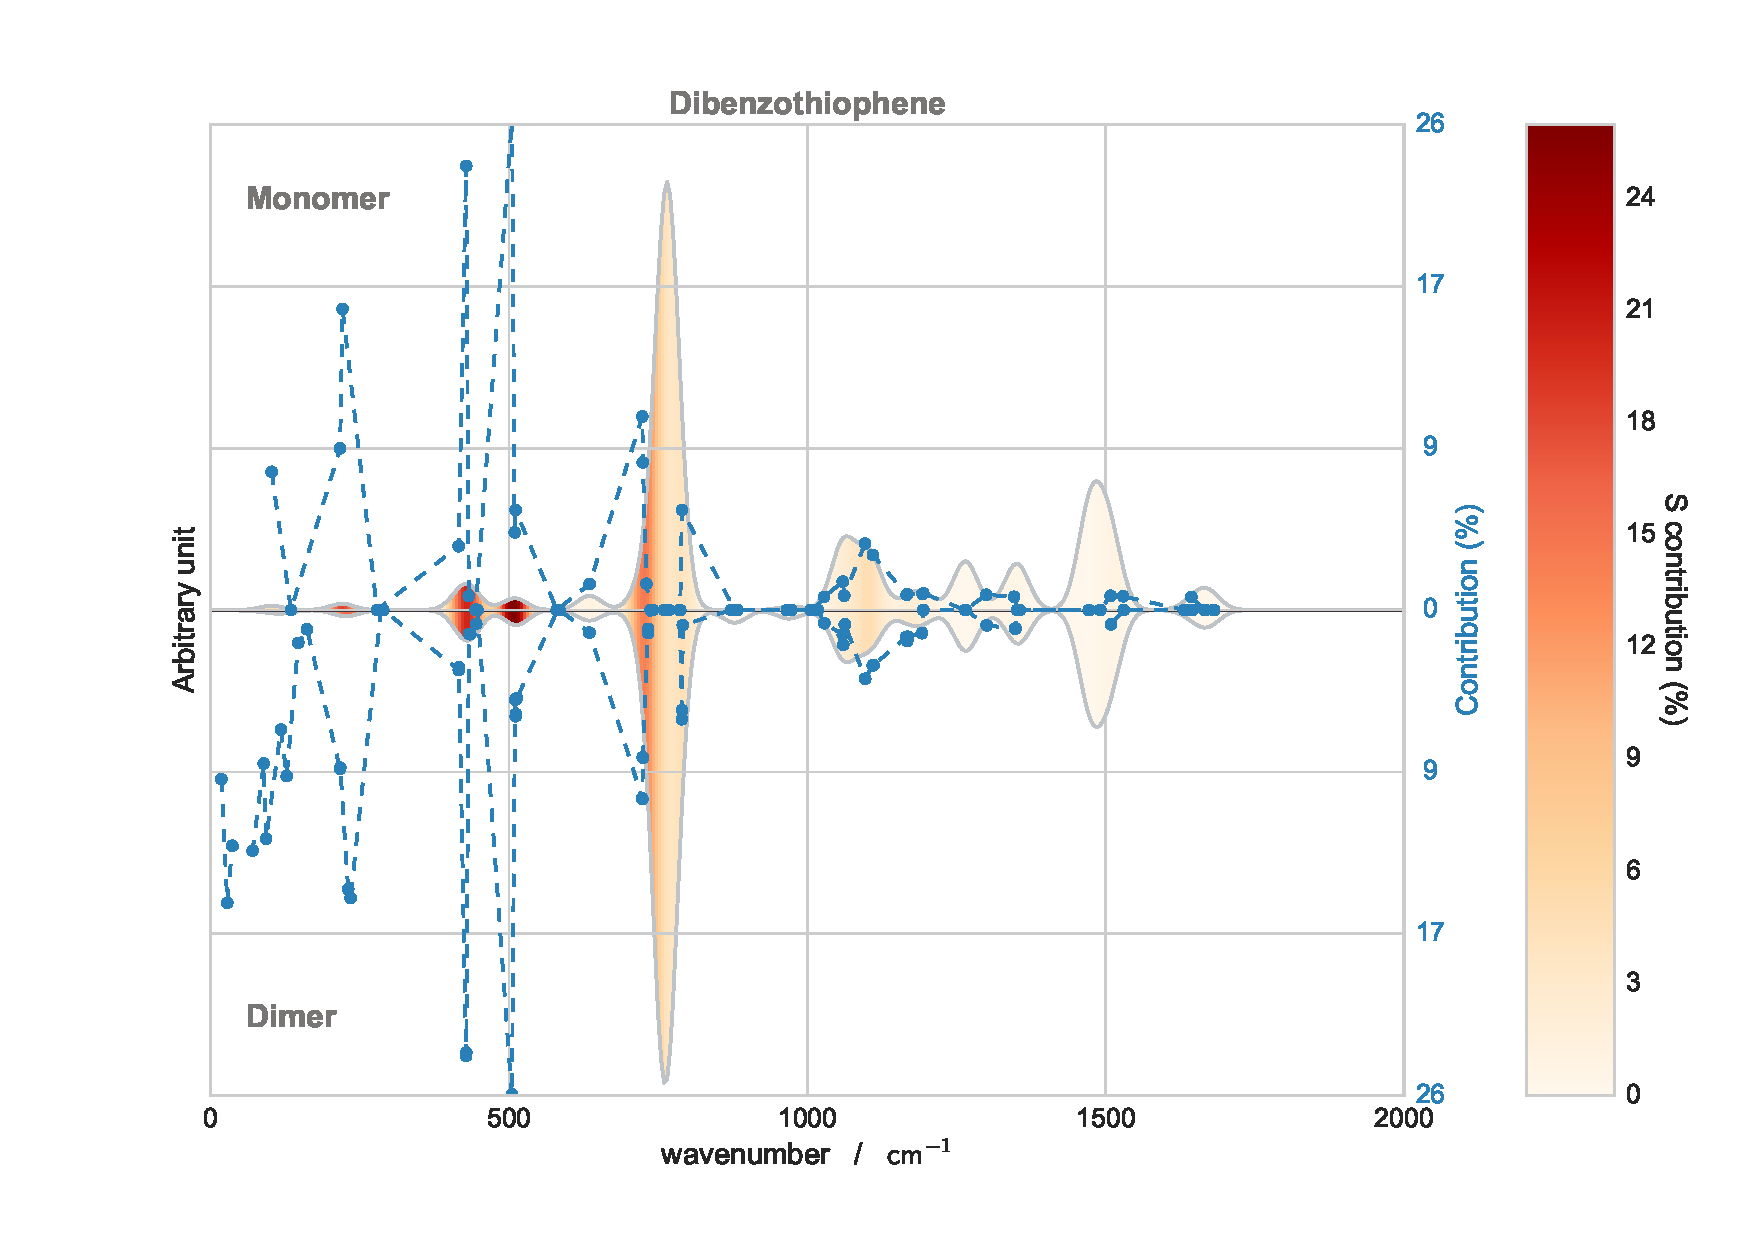
\includegraphics[scale=0.4]{image/P2-13}
		\end{center}
		\caption{Monomer and dimer comparison of calculated vibrational spetra of Dibenzothiophene} \label{figP2-13}
	\end{figure}
	
		Analysing the 0-800 cm$^{-1}$ spectral zone for which we had particularly noted modifications (on frequencies and intensities) due to the wagging of nitrogen shows now no particularity when we have sulphur as hetero atom, neither for frequency’s positioning (figure \ref{figP2-14}) nor mode densities (figure \ref{figP2-15}). In any case and for all the spectral zones, there is an excellent theory-experiment agreement. The strong similarities found for dibenzothiophene’s monomer and dimer show that it is probably not possible to discriminate spectroscopically the presence of associated systems, exception made for the spectral zone $x_3=1$ relative to the \textit{inter}-molecular modes and the ones coupled to them, such as the butterfly ones).
	
	
		\begin{figure}[H]
			\begin{center}
				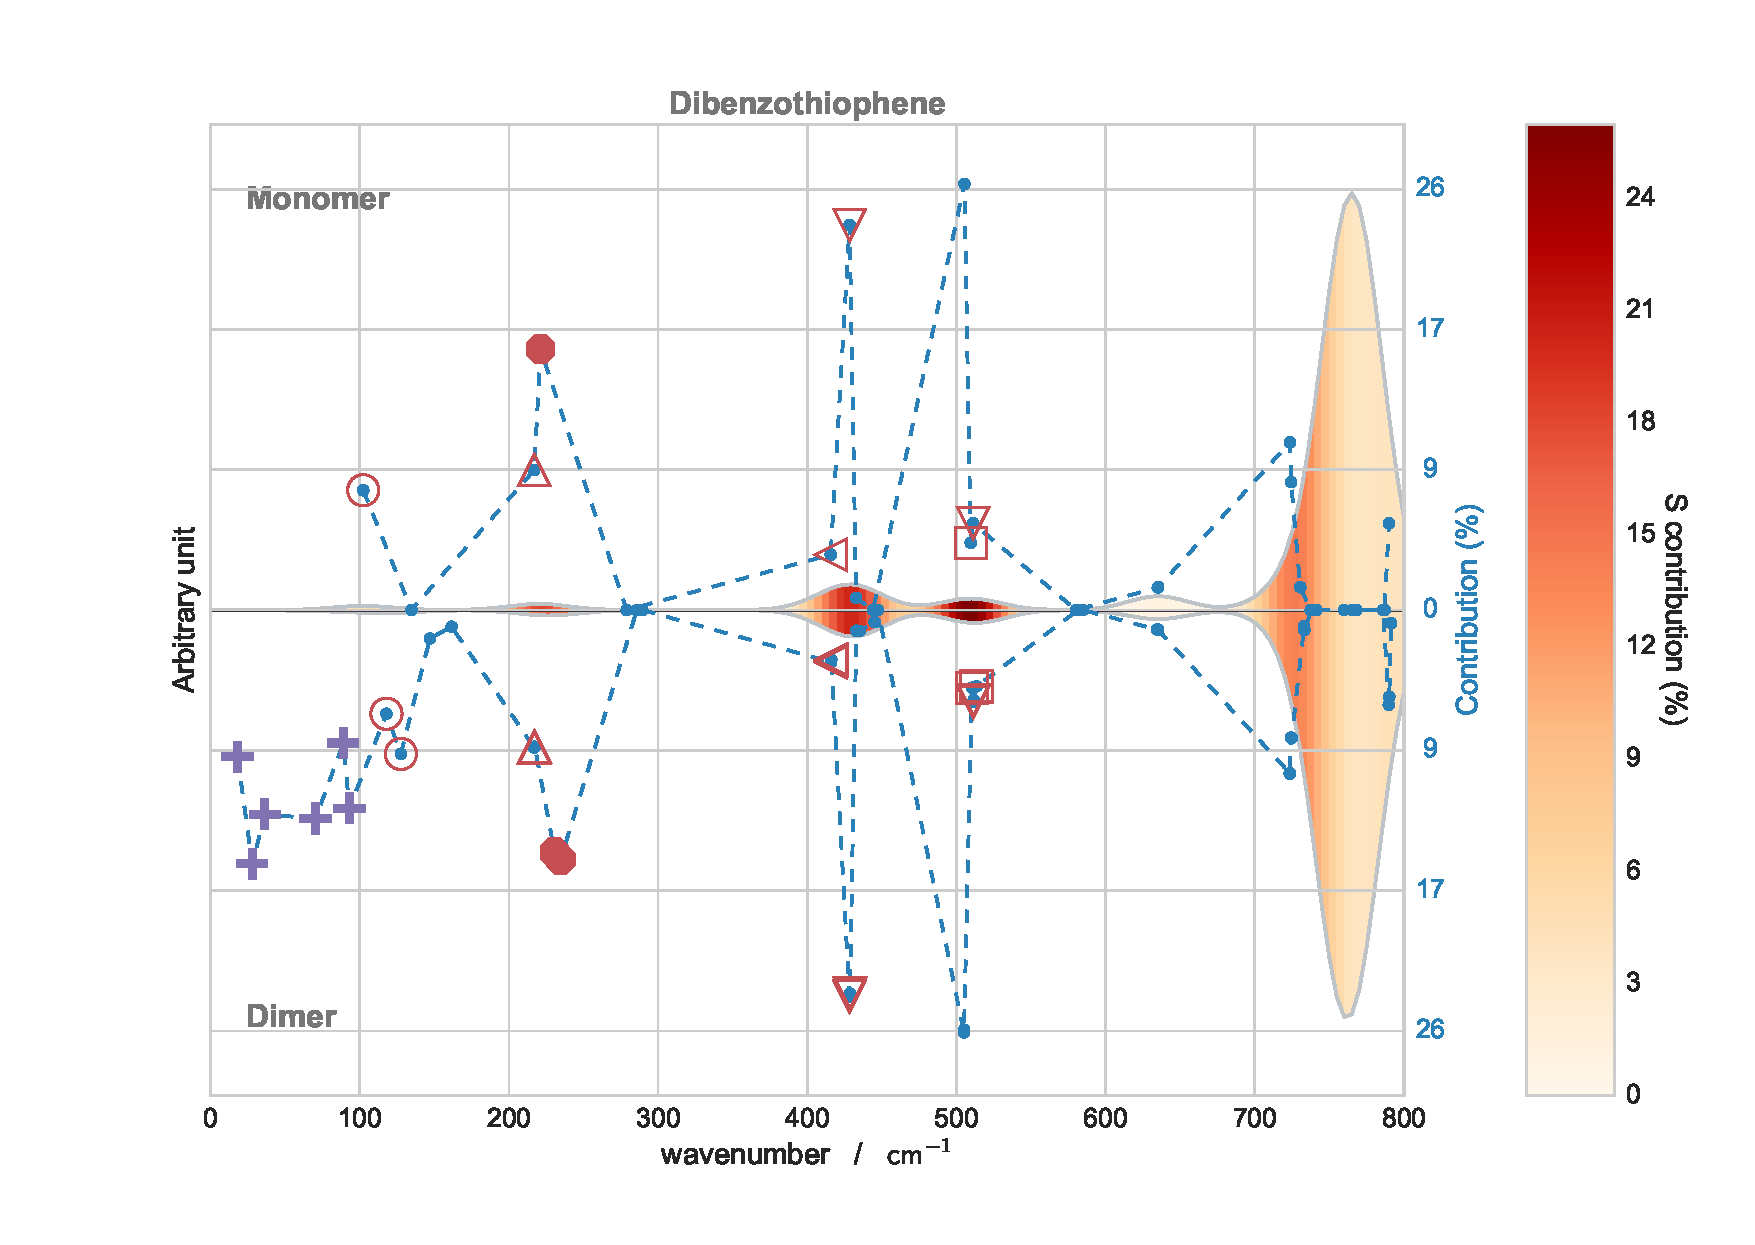
\includegraphics[scale=0.4]{image/P2-14}
			\end{center}
			\caption{Calculated vibrational spectra of Carbazole monomer and dimer, between 0- 800 cm$^{-1}$, showing heteroatom contribution and important modes.} \label{figP2-14}
		\end{figure}
		
		
			\begin{figure}[H]
				\begin{center}
					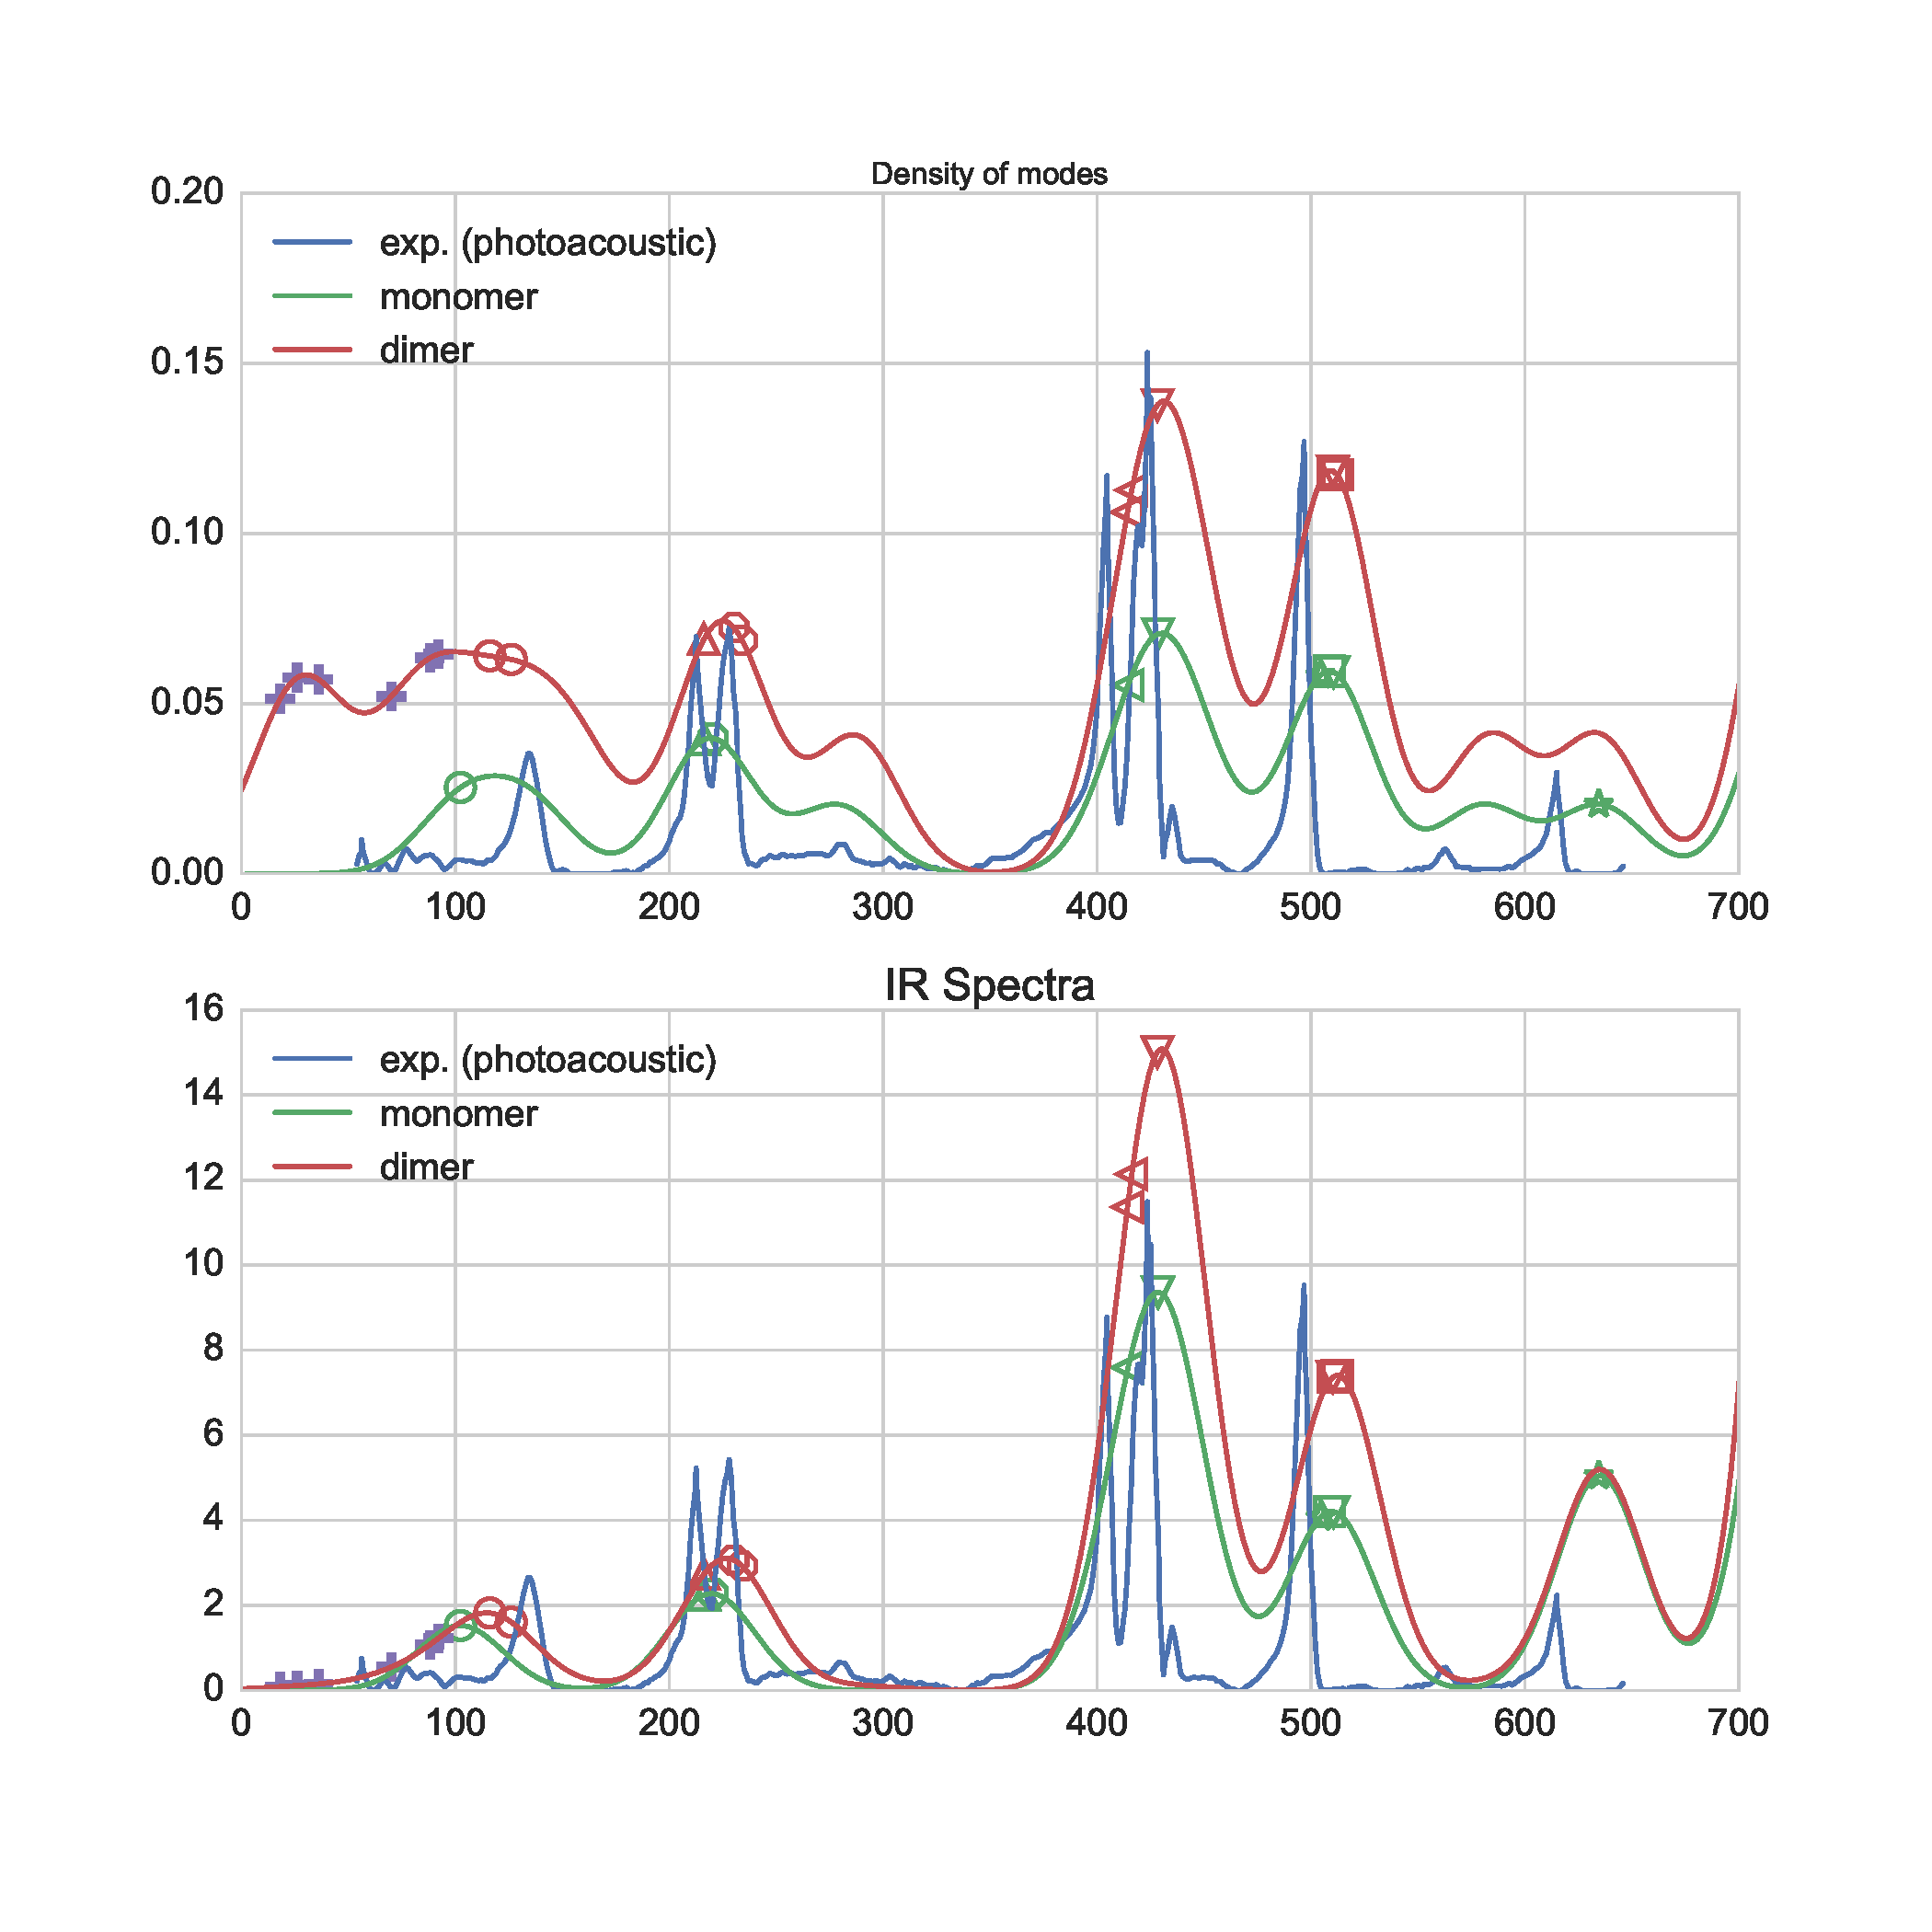
\includegraphics[scale=0.31]{image/P2-15}
				\end{center}
				\caption{Comparison between monomer, dimer calculated and experimental spectra, Densite of modes at the top and normal vibrational modes and IR intensities at the bottom.} \label{figP2-15}
			\end{figure}
	

	These ensembles of conclusions are also valid for all the other molecules of the thiophene family (figure \ref{figP2-16ad}). They also apply to the ensemble of molecules studied in this work having oxygen or carbon as heteroatom (figure \ref{figP2-17ae} and \ref{figP2-18ae}). Finally, apart the \textit{inter}-molecular modes and the ones that are coupled with them, only the N-H wagging mode for the molecules of the nitrogen family have enough singularities to allow the discrimination of the monomeric and associated states.
	
		
		\begin{figure}[H]
			\begin{center}
				\resizebox{17cm}{!}{
					\begin{tabular}{c c}
						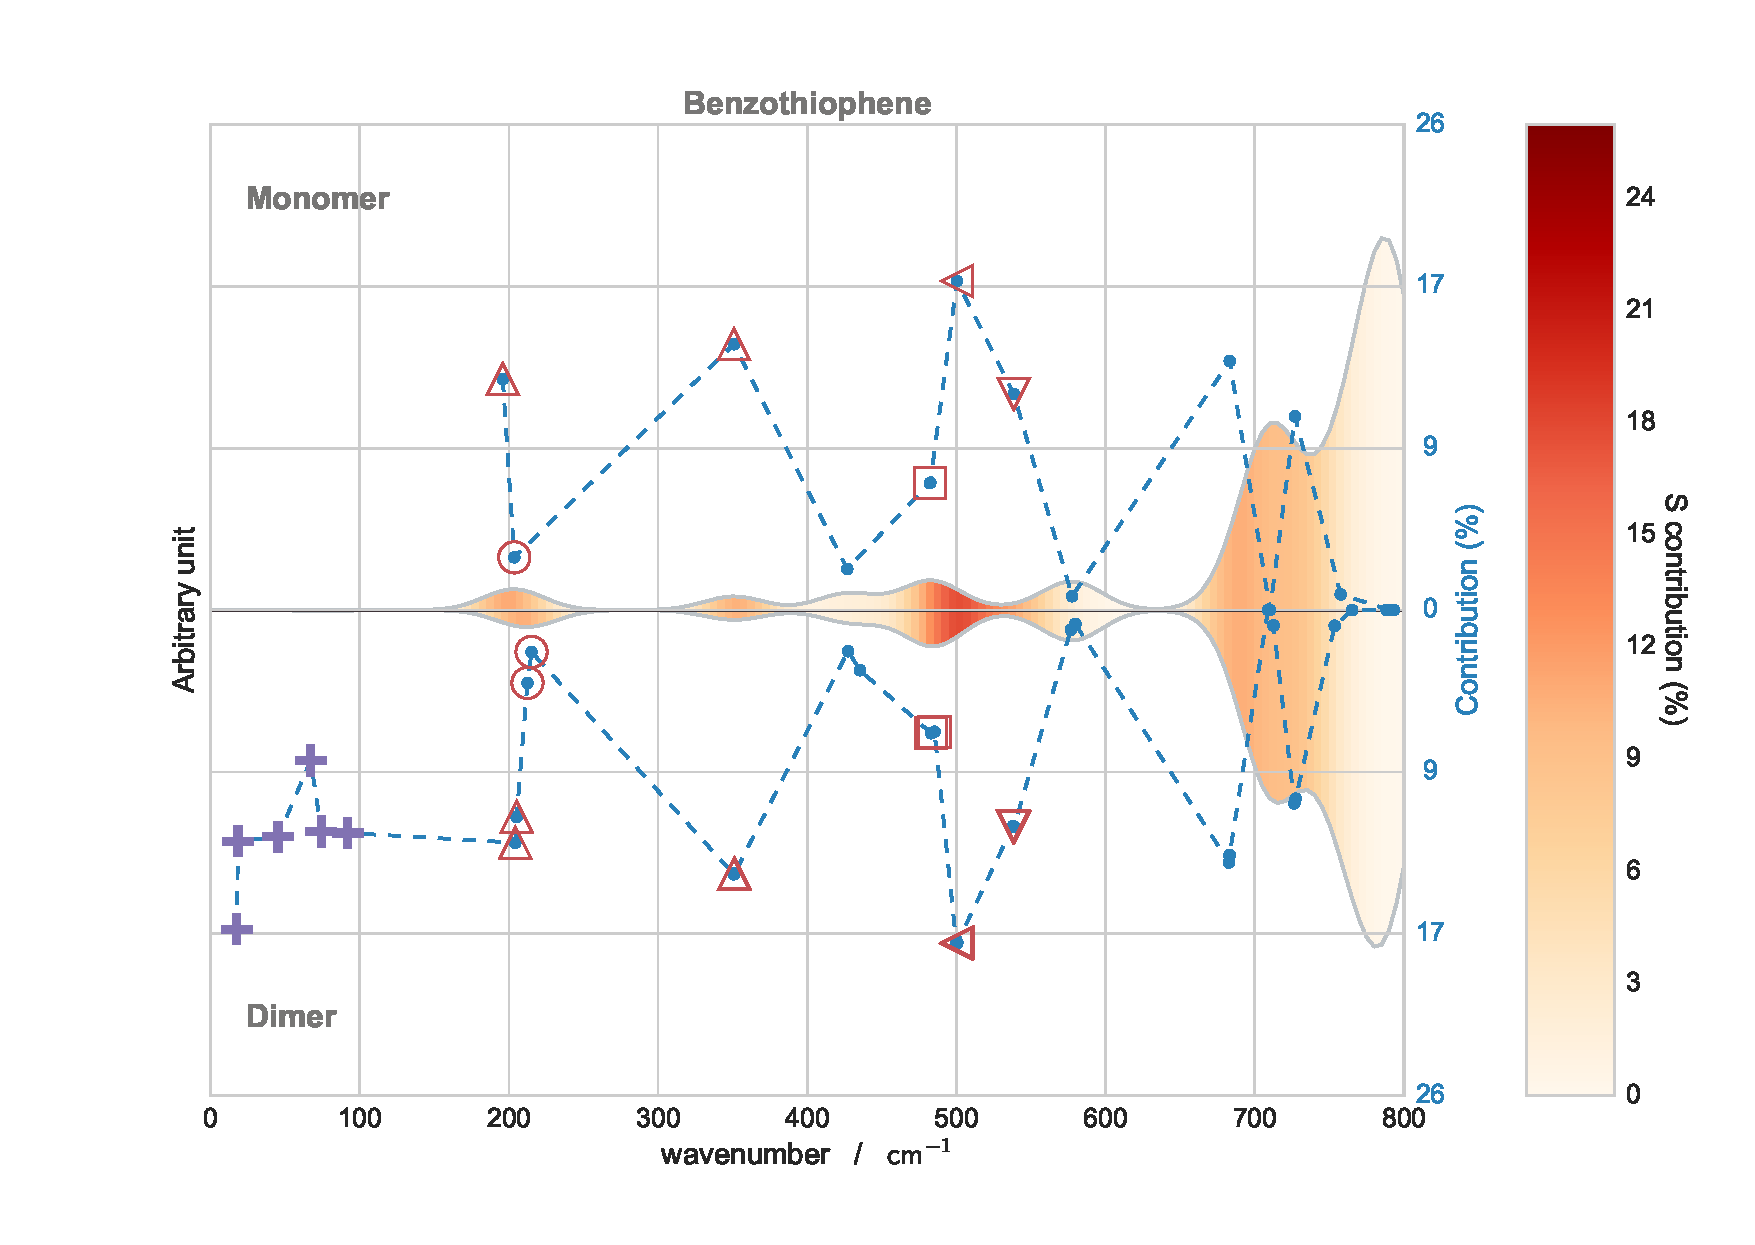
\includegraphics[scale=0.3]{image/P2-16a} & 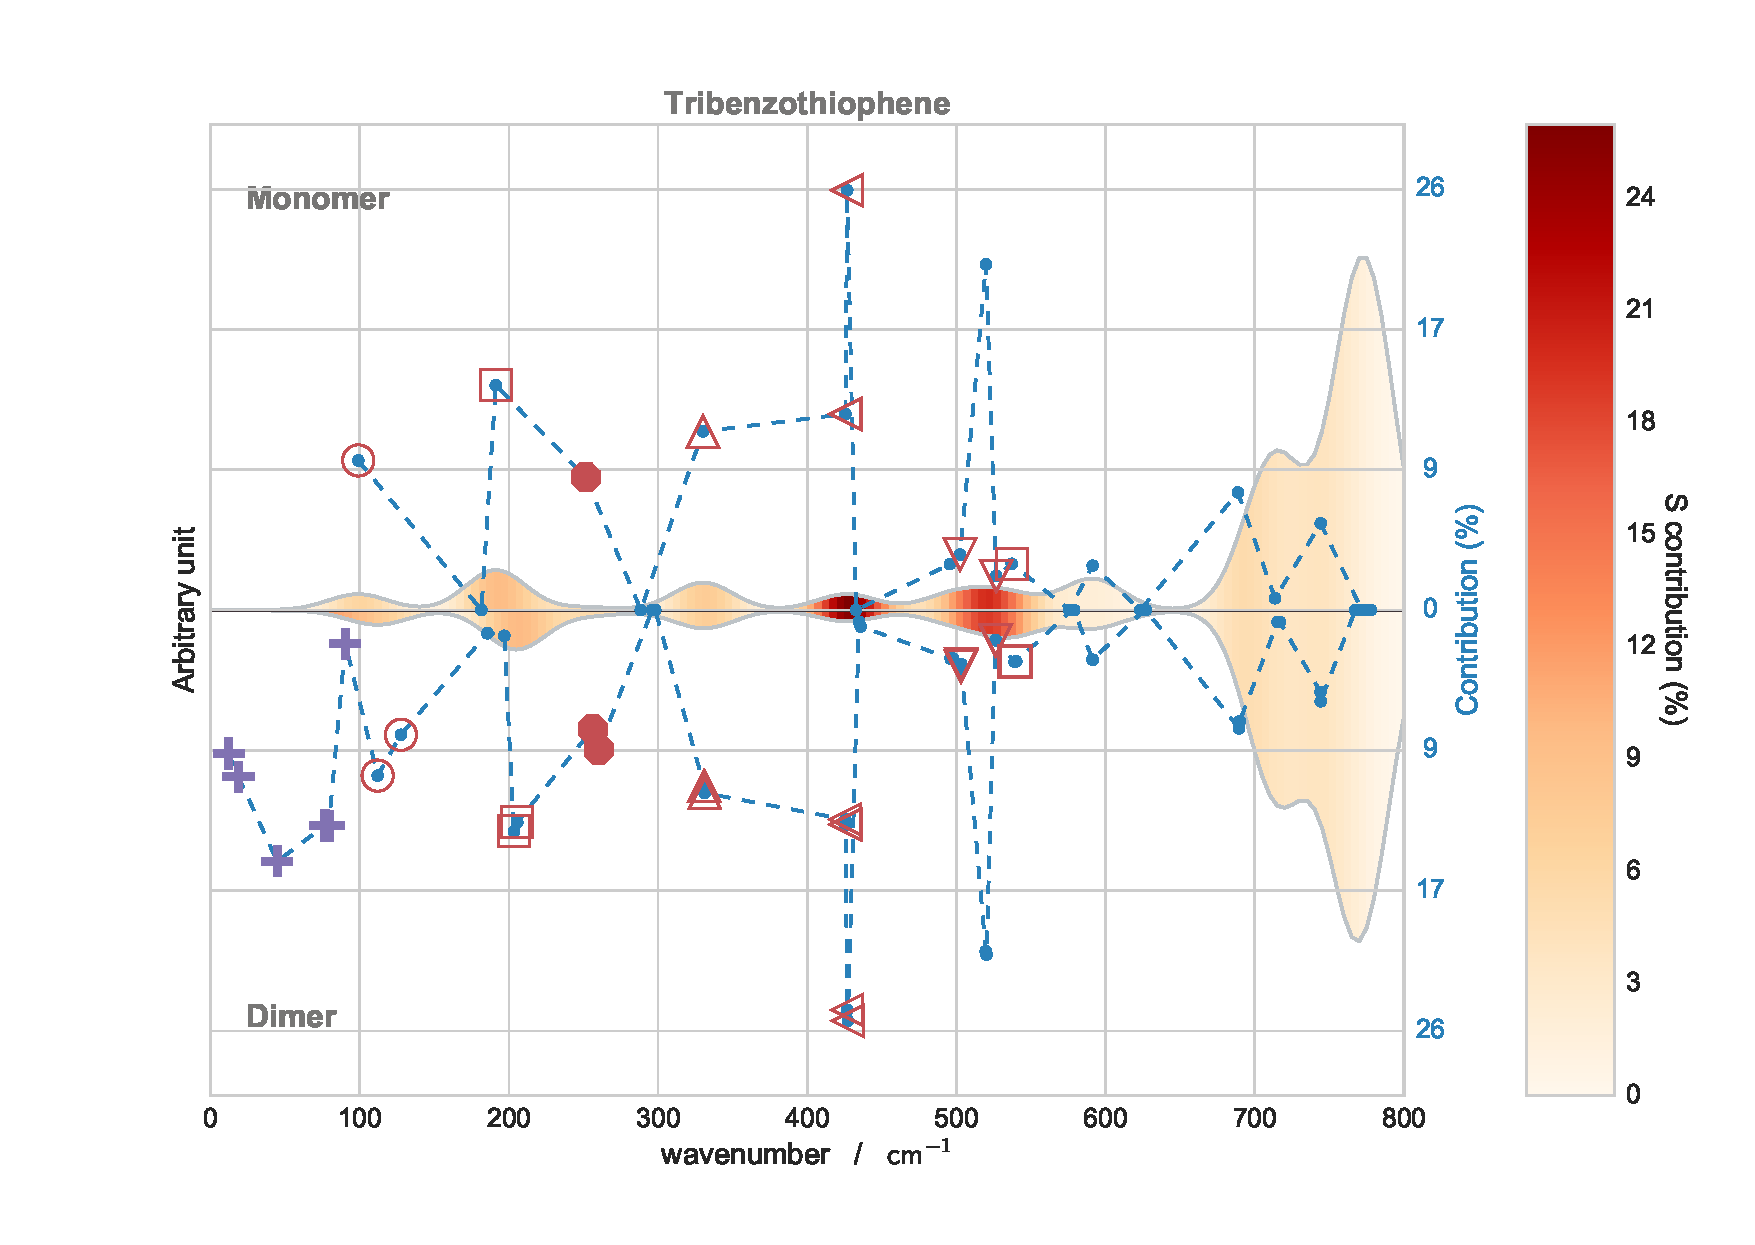
\includegraphics[scale=0.3]{image/P2-16b} \\
						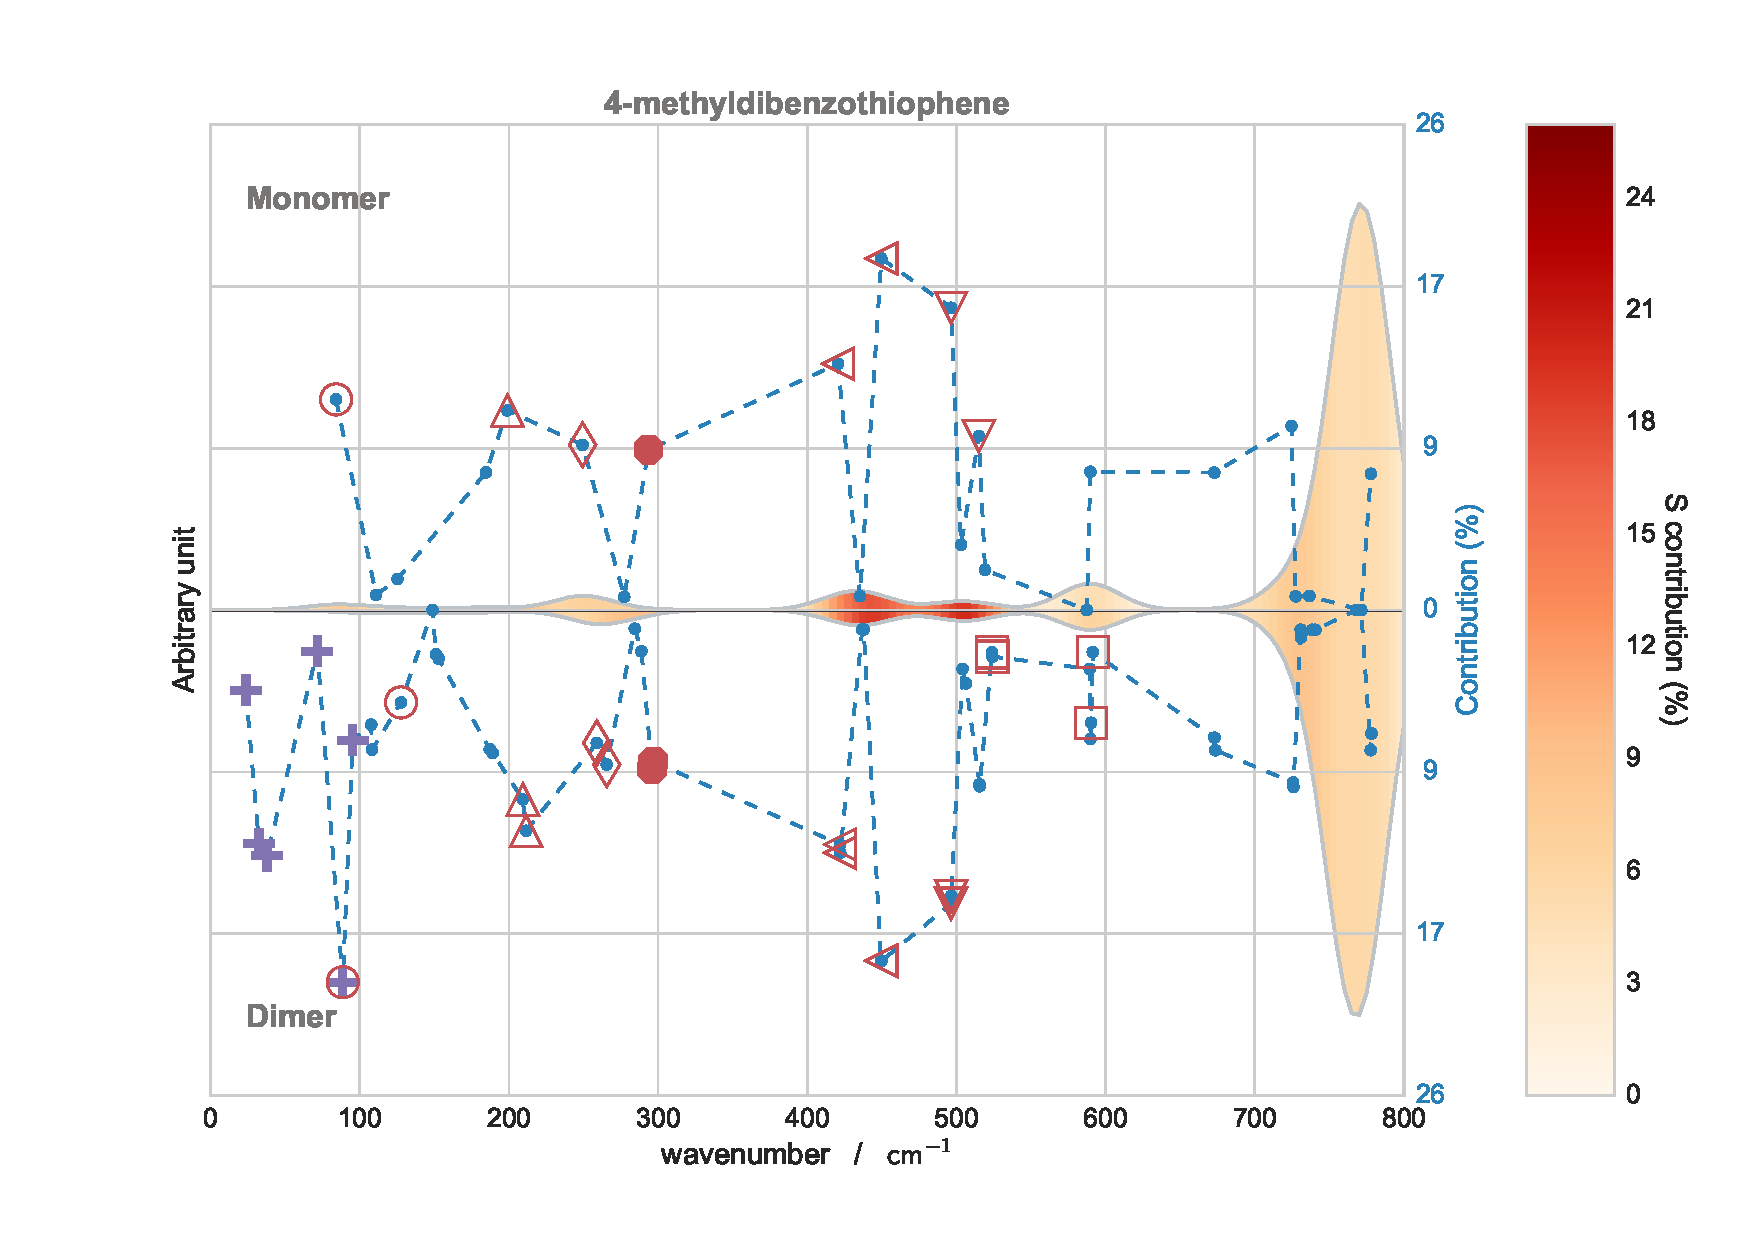
\includegraphics[scale=0.3]{image/P2-16c} & 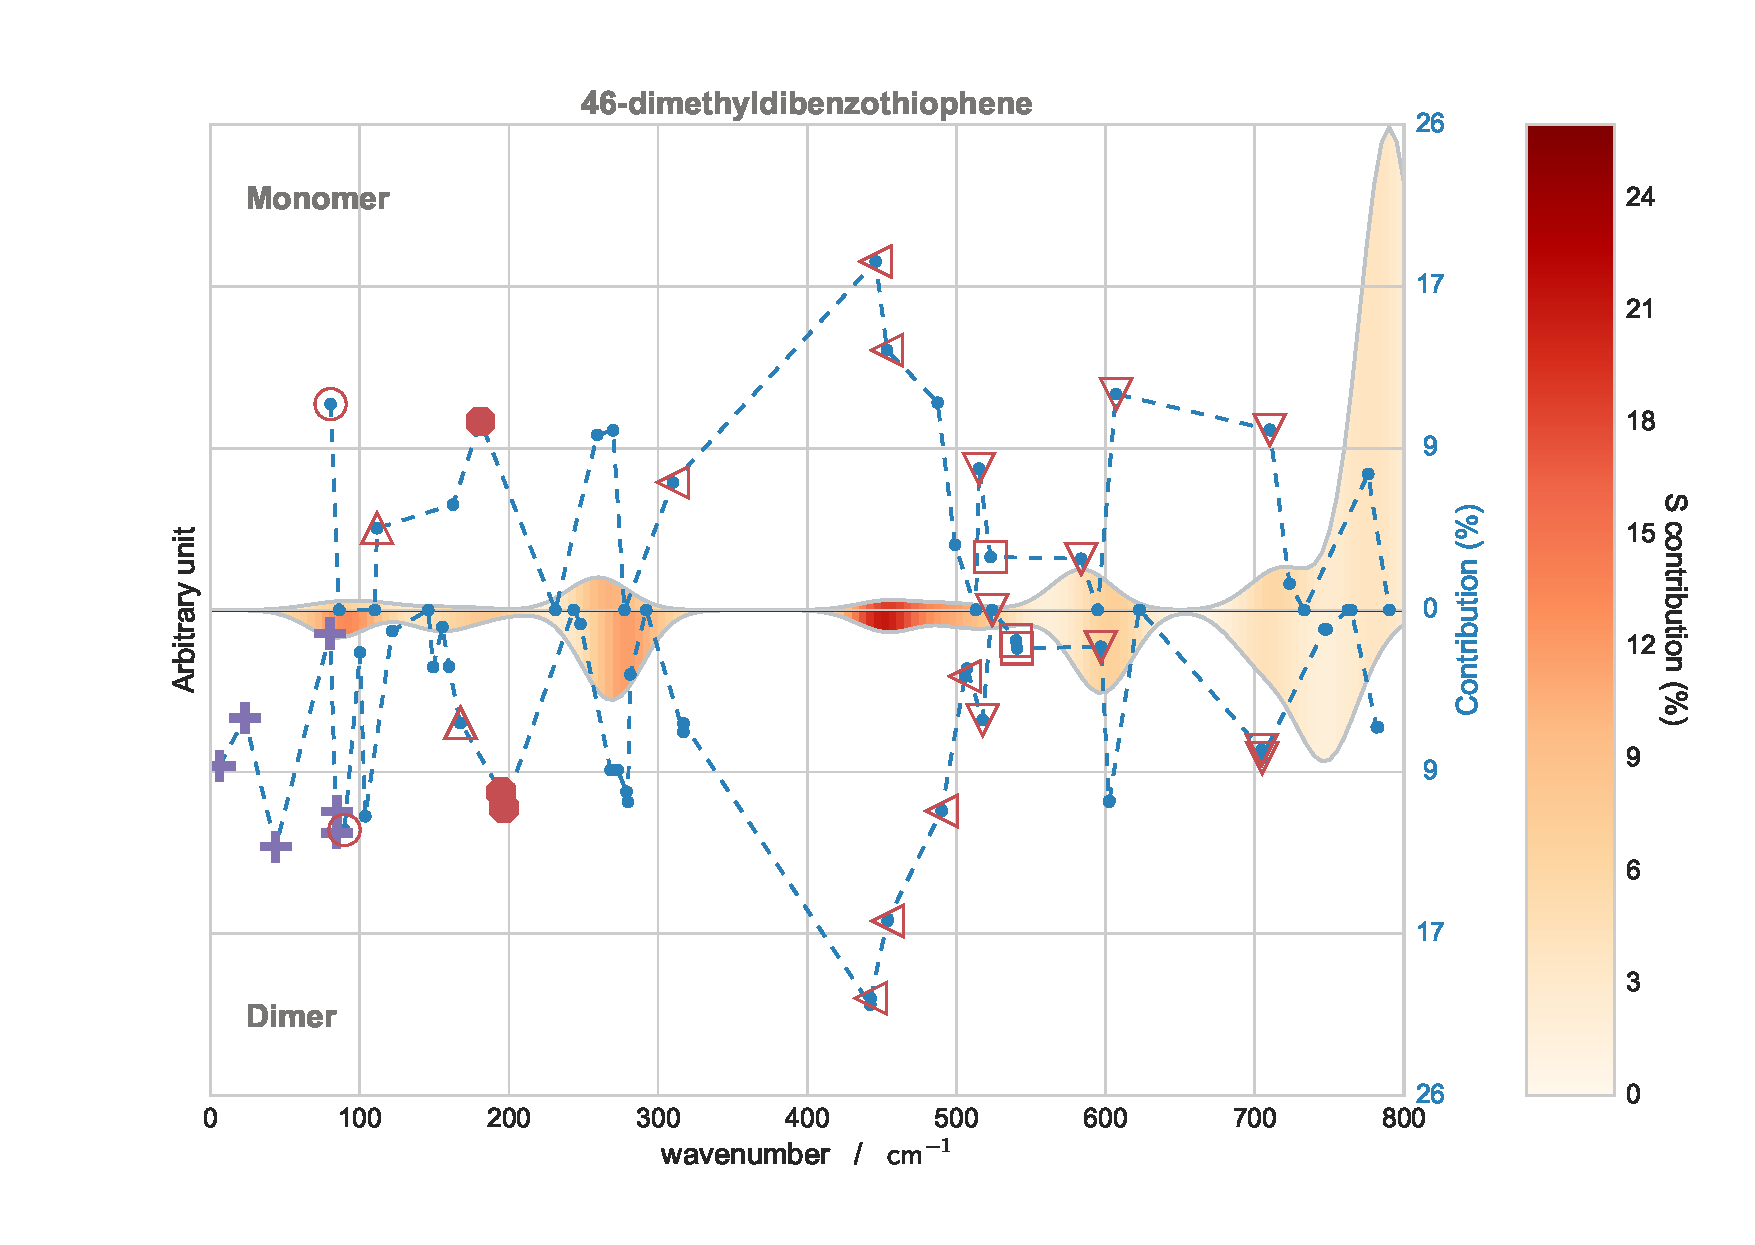
\includegraphics[scale=0.3]{image/P2-16d}\\
					\end{tabular}}
				\end{center}
				\caption{Comparison between momoner and dimer calculated vibrational spectra for \textbf{a} Benzothiophene, \textbf{b} Tribenzothiophene, \textbf{c} 4-methyldibenzothiophene and \textbf{d} 4,6-dimethyldibenzothiophene at 0- 800 cm$^{-1}$ interval.}  \label{figP2-16ad}
			\end{figure}
	
	
	\begin{figure}[H]
		\begin{center}
			\resizebox{17cm}{!}{
				\begin{tabular}{c c}
					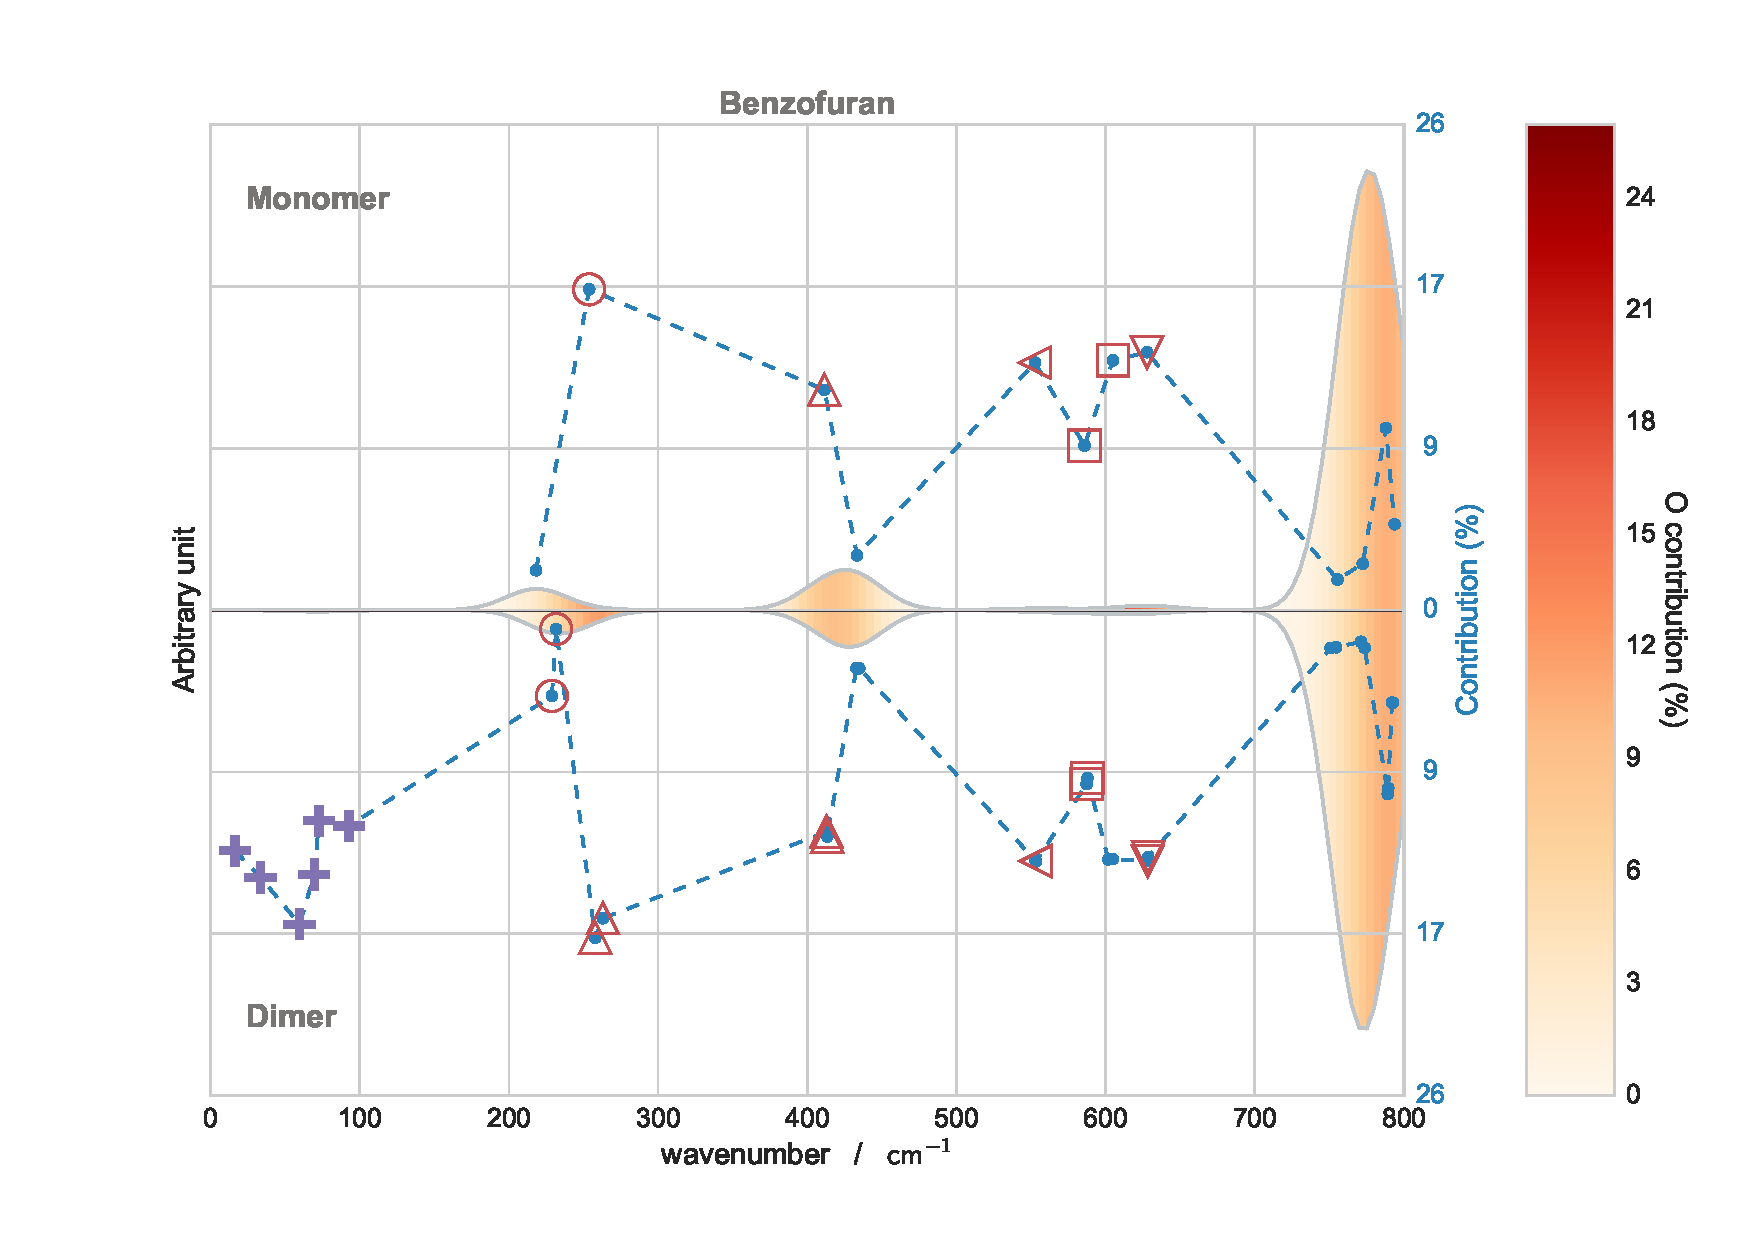
\includegraphics[scale=0.3]{image/P2-17a} & 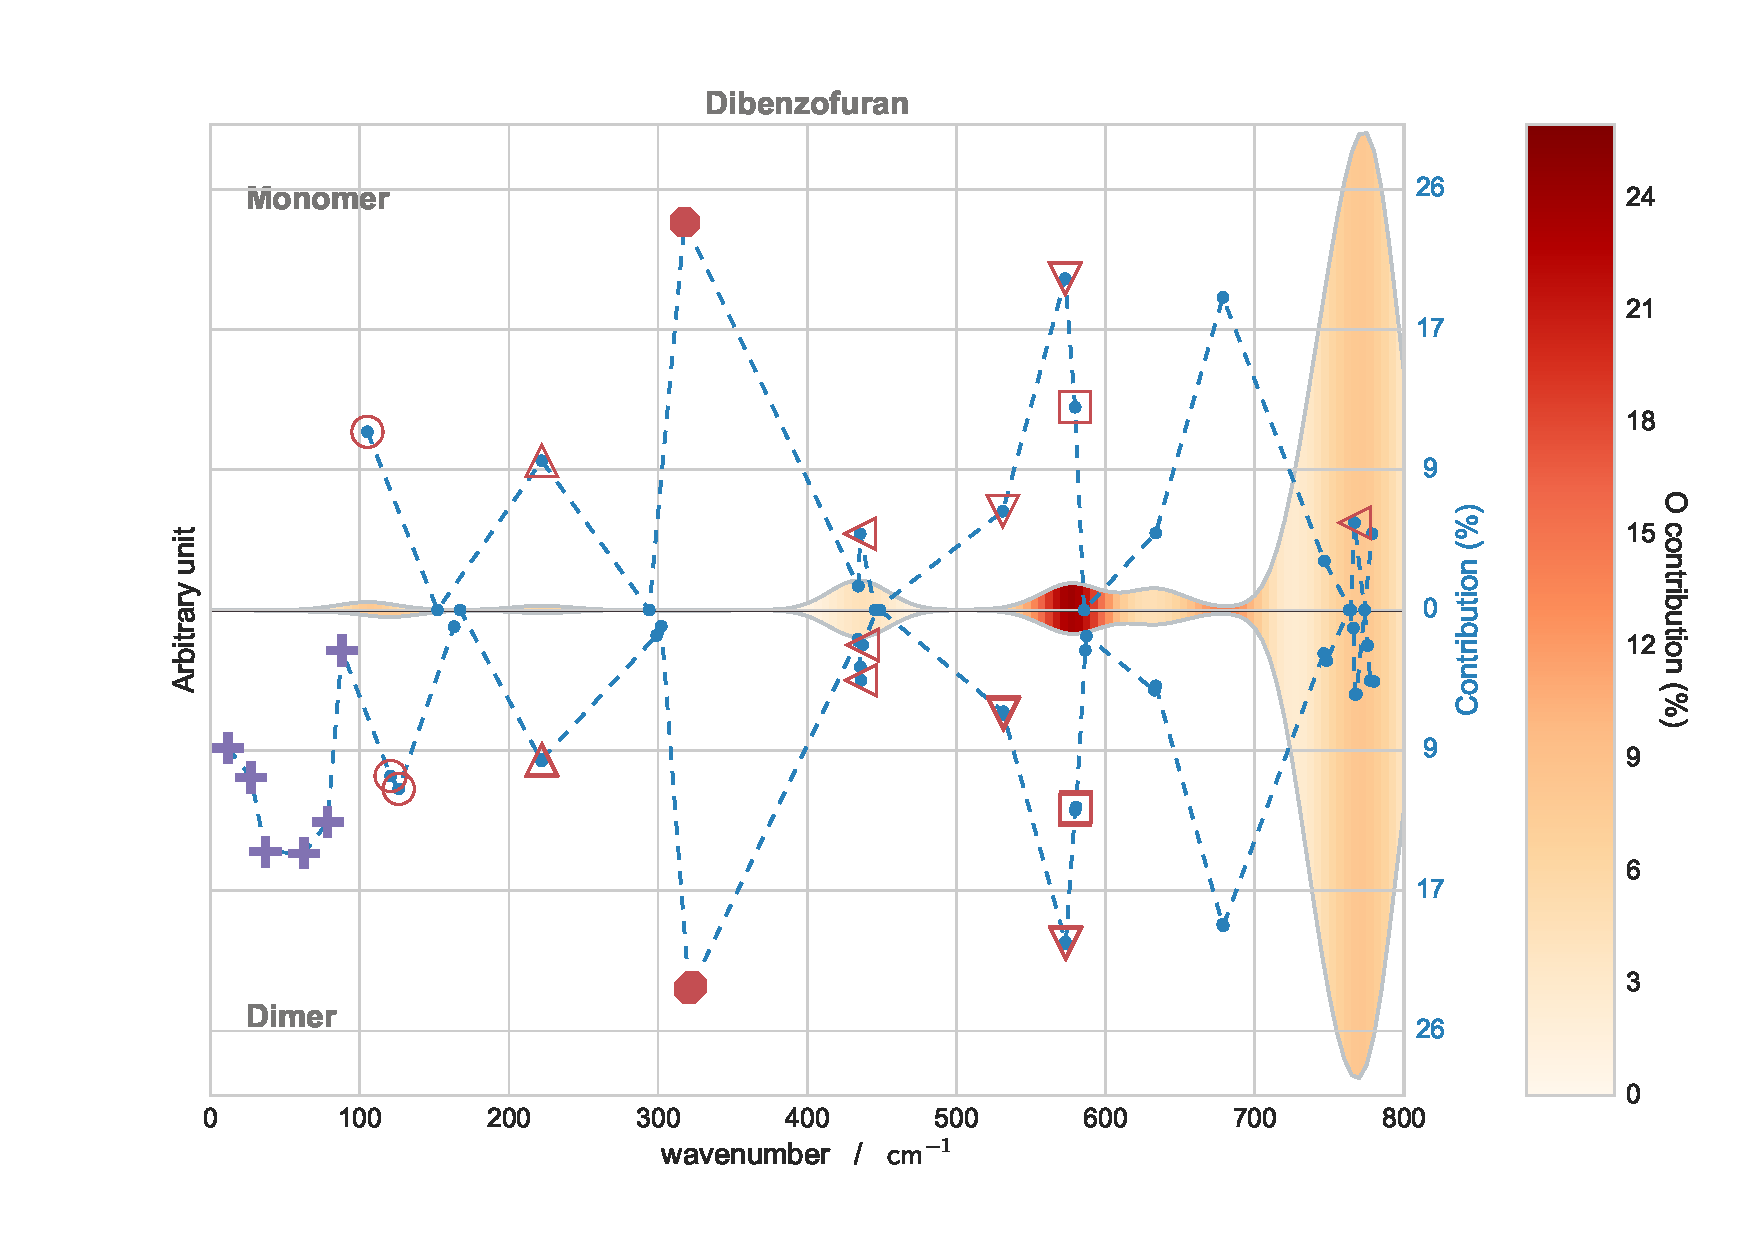
\includegraphics[scale=0.3]{image/P2-17b} \\
					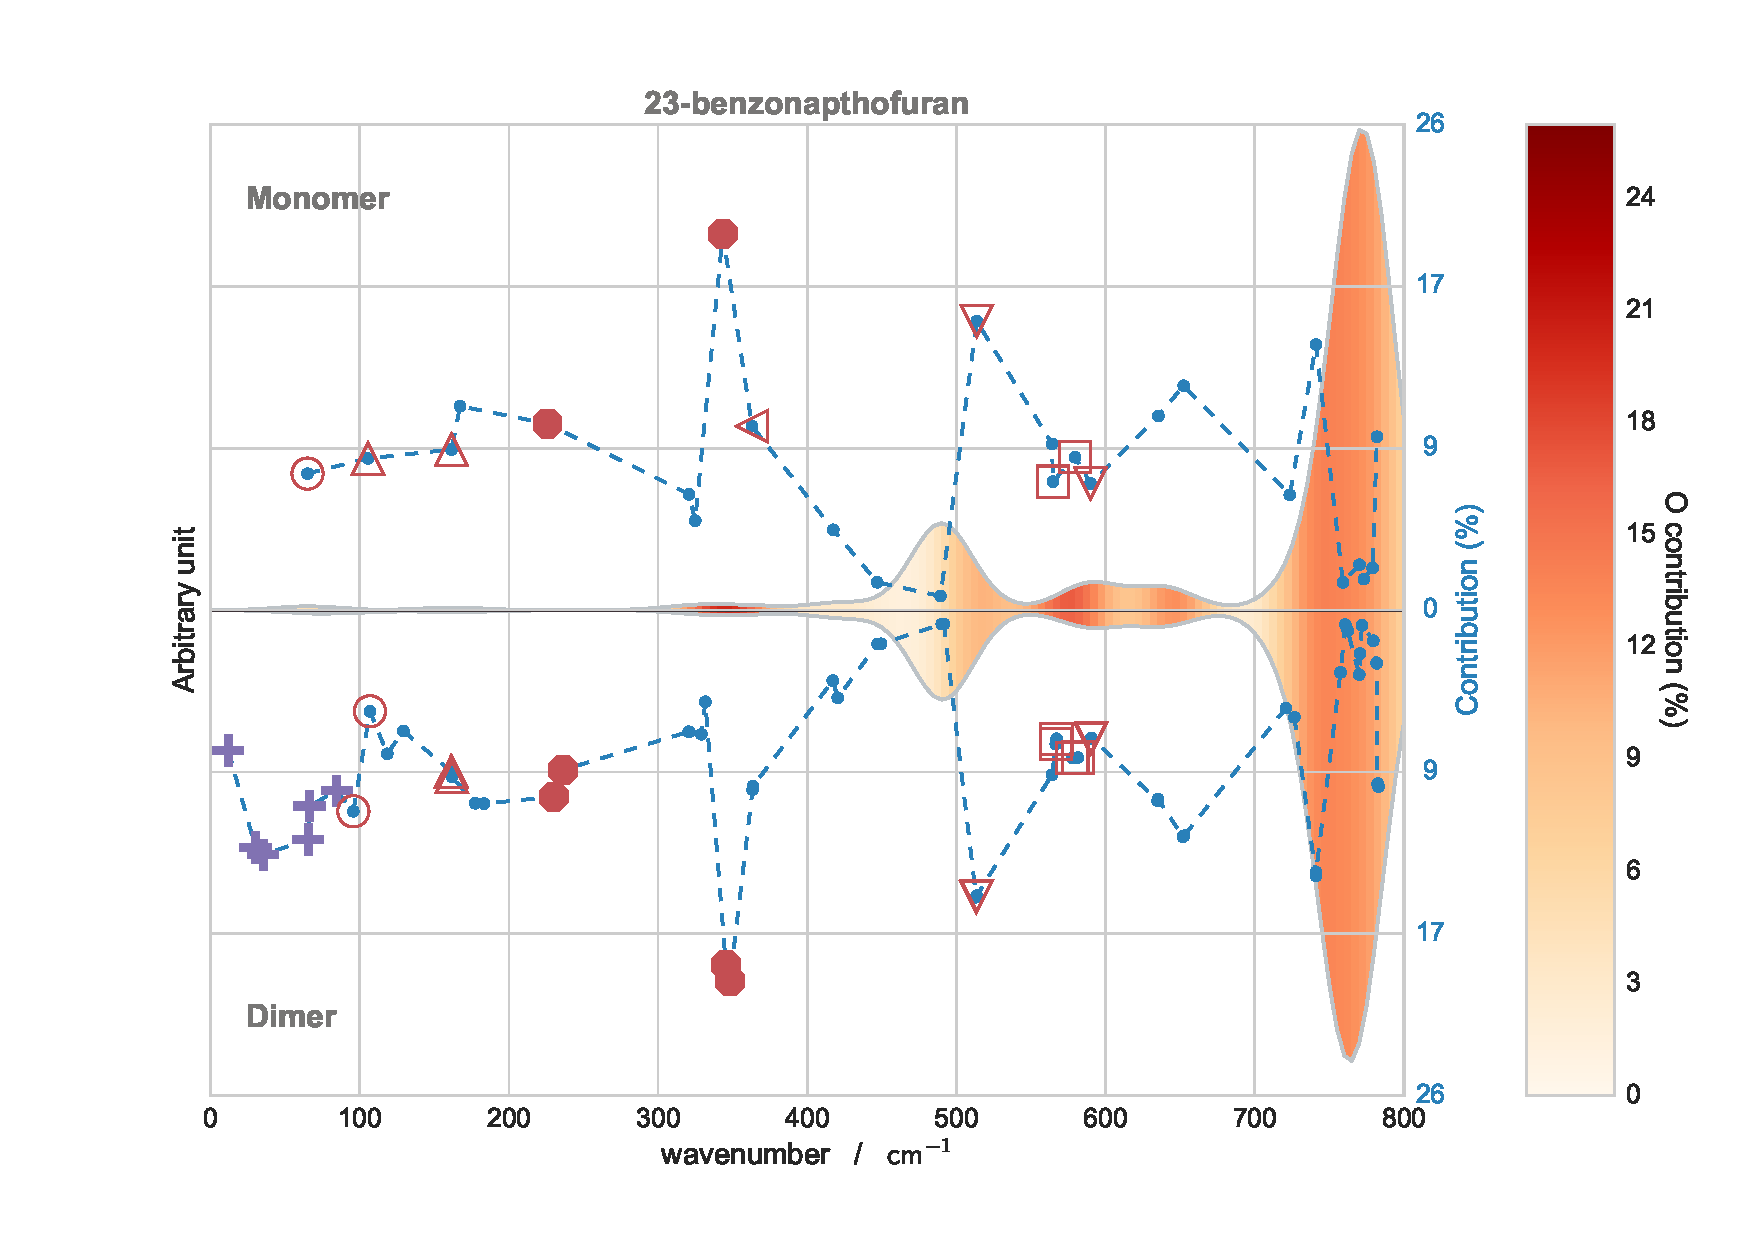
\includegraphics[scale=0.3]{image/P2-17c1} & 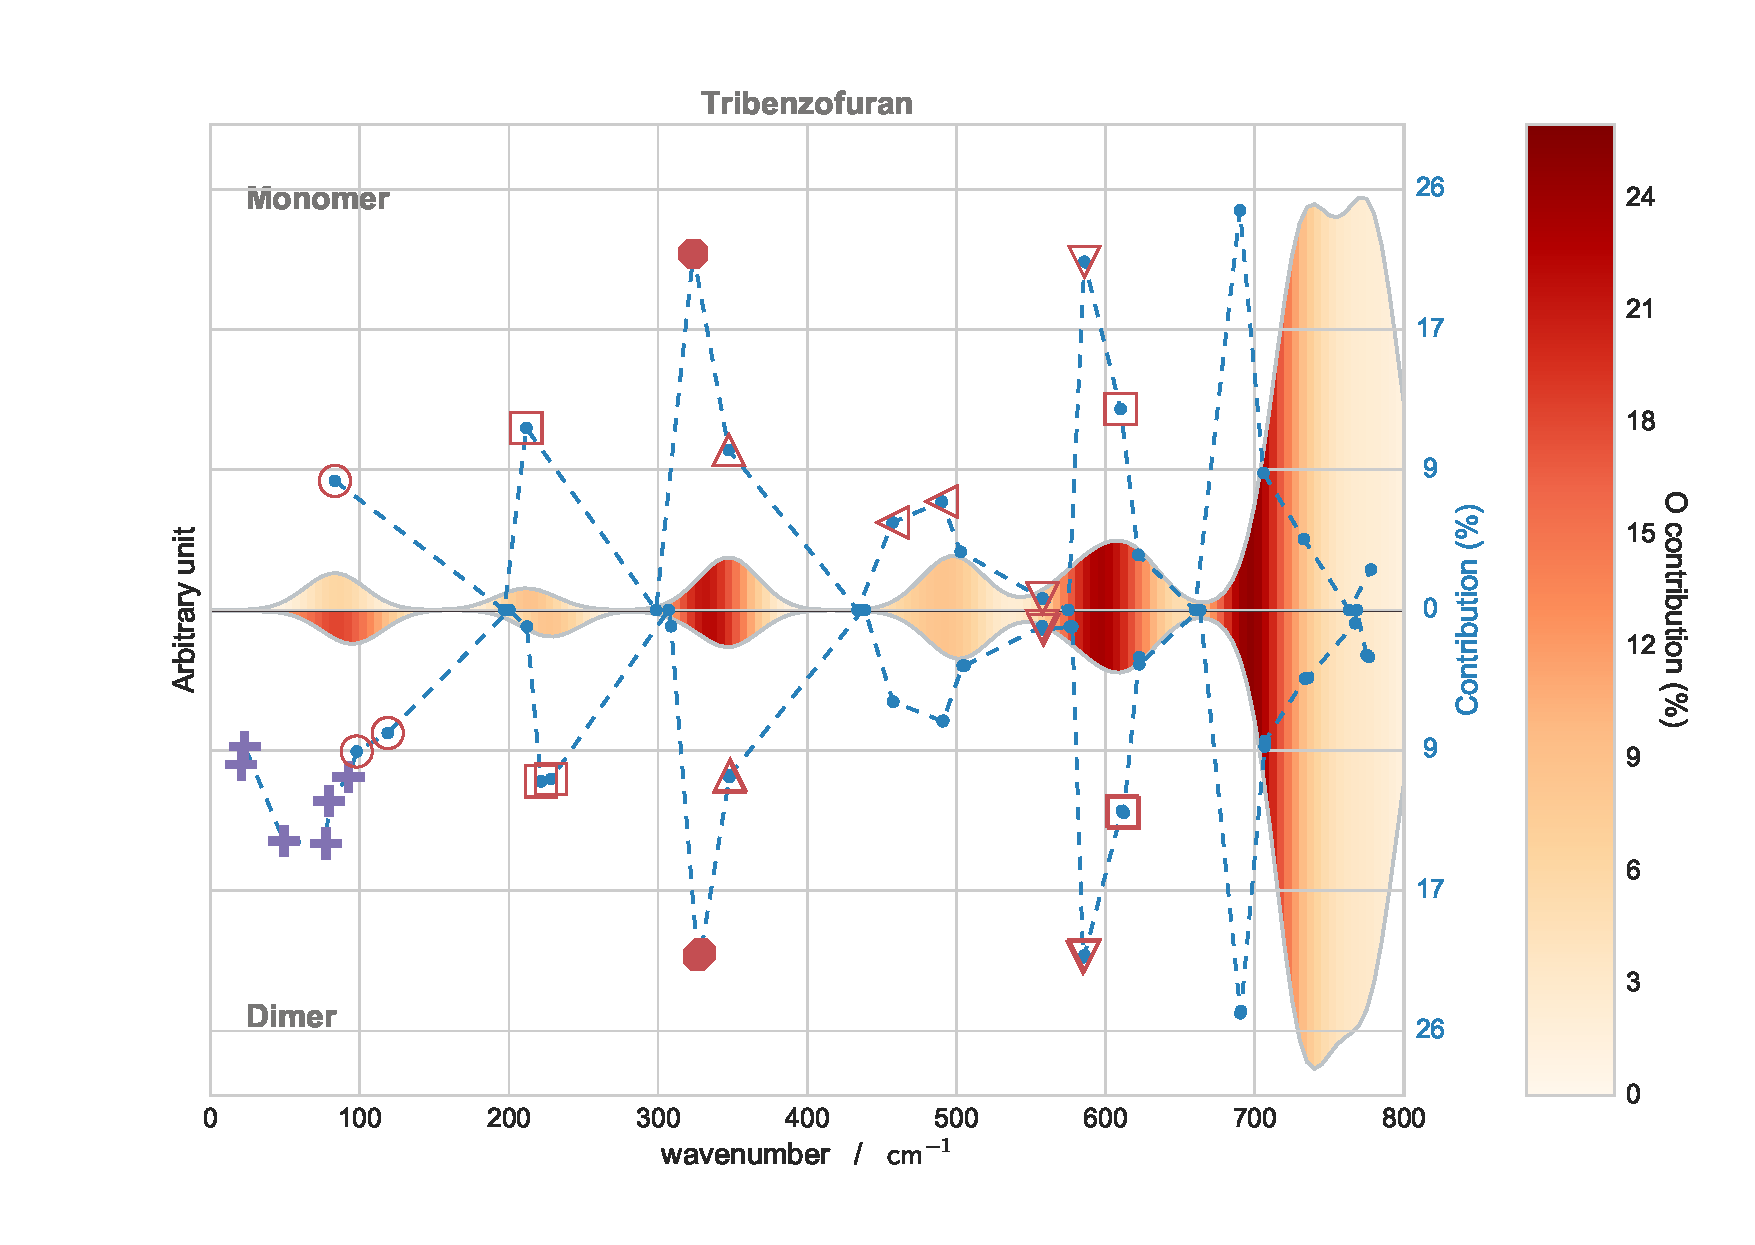
\includegraphics[scale=0.3]{image/P2-17c}\\
					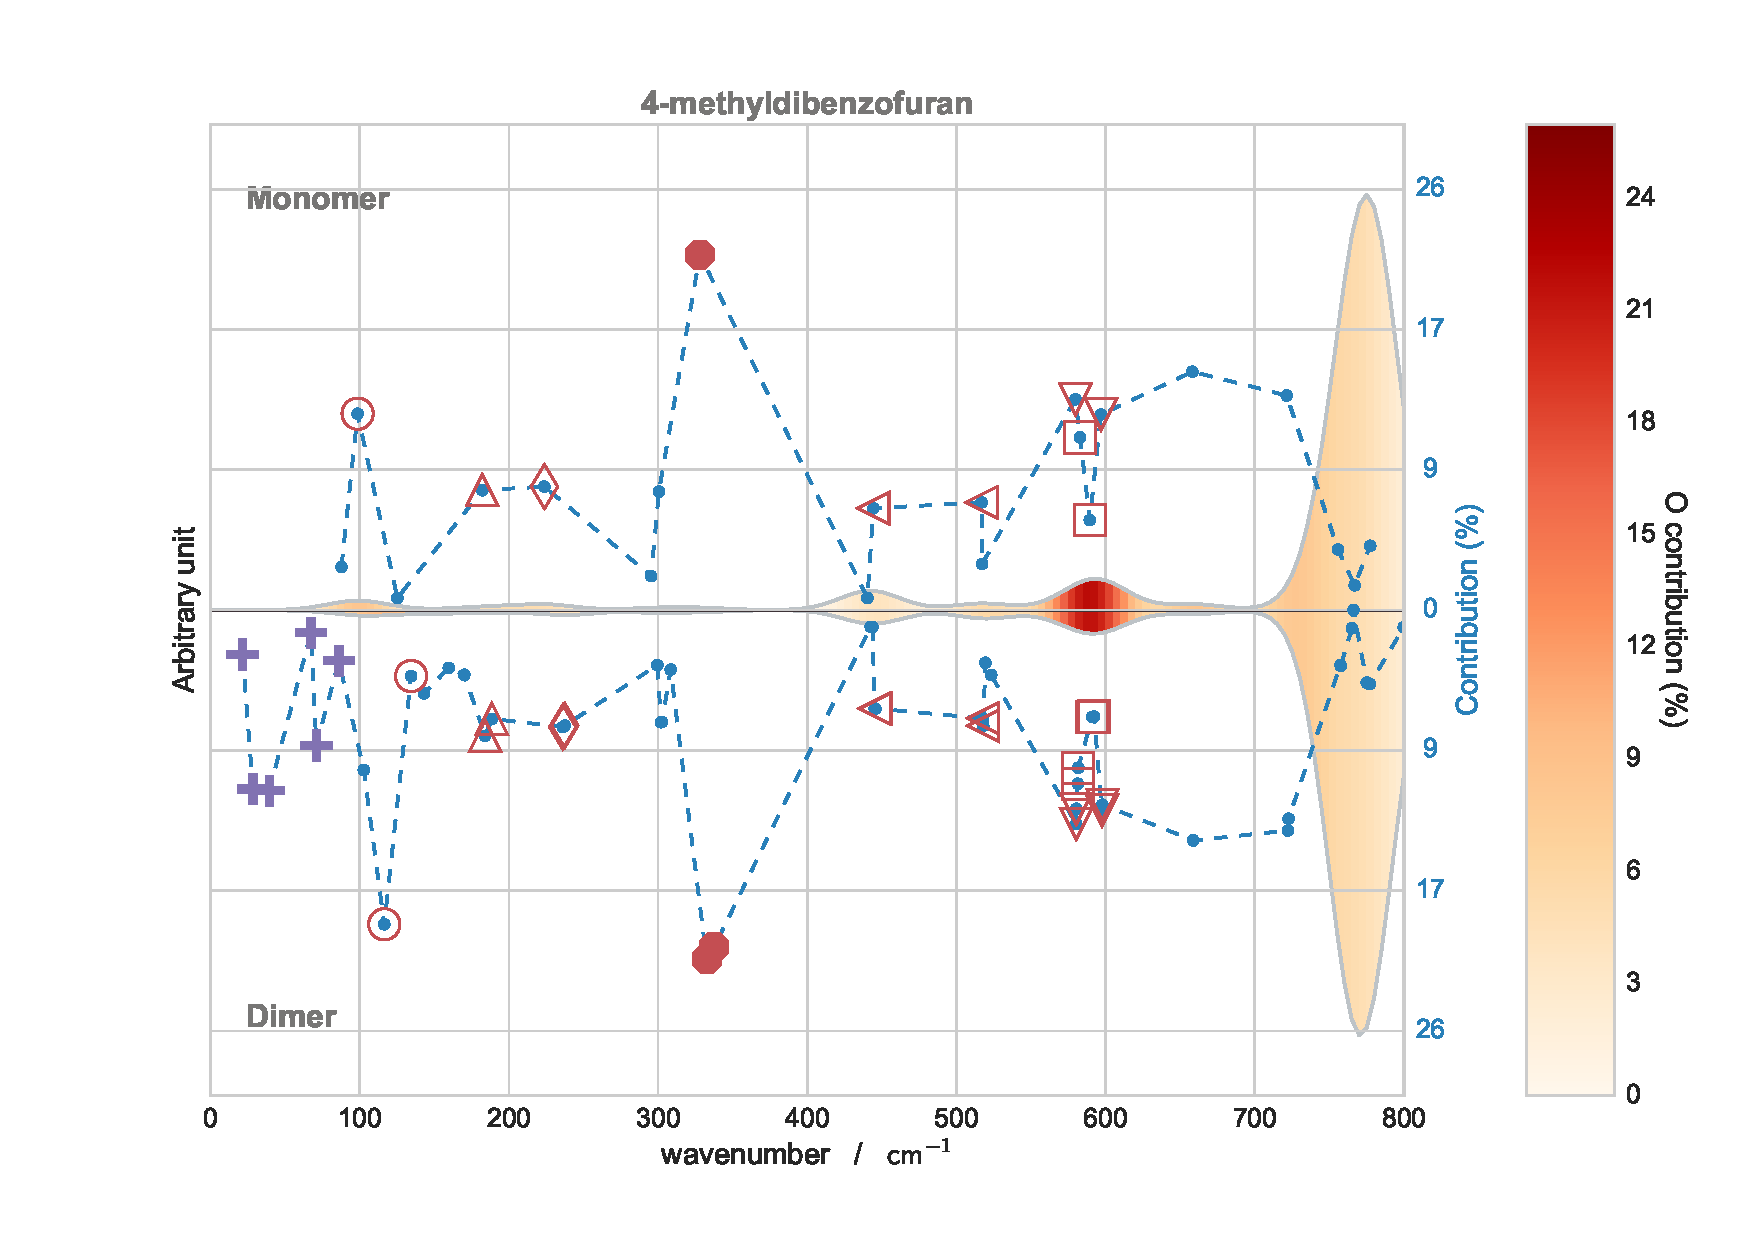
\includegraphics[scale=0.3]{image/P2-17d} & 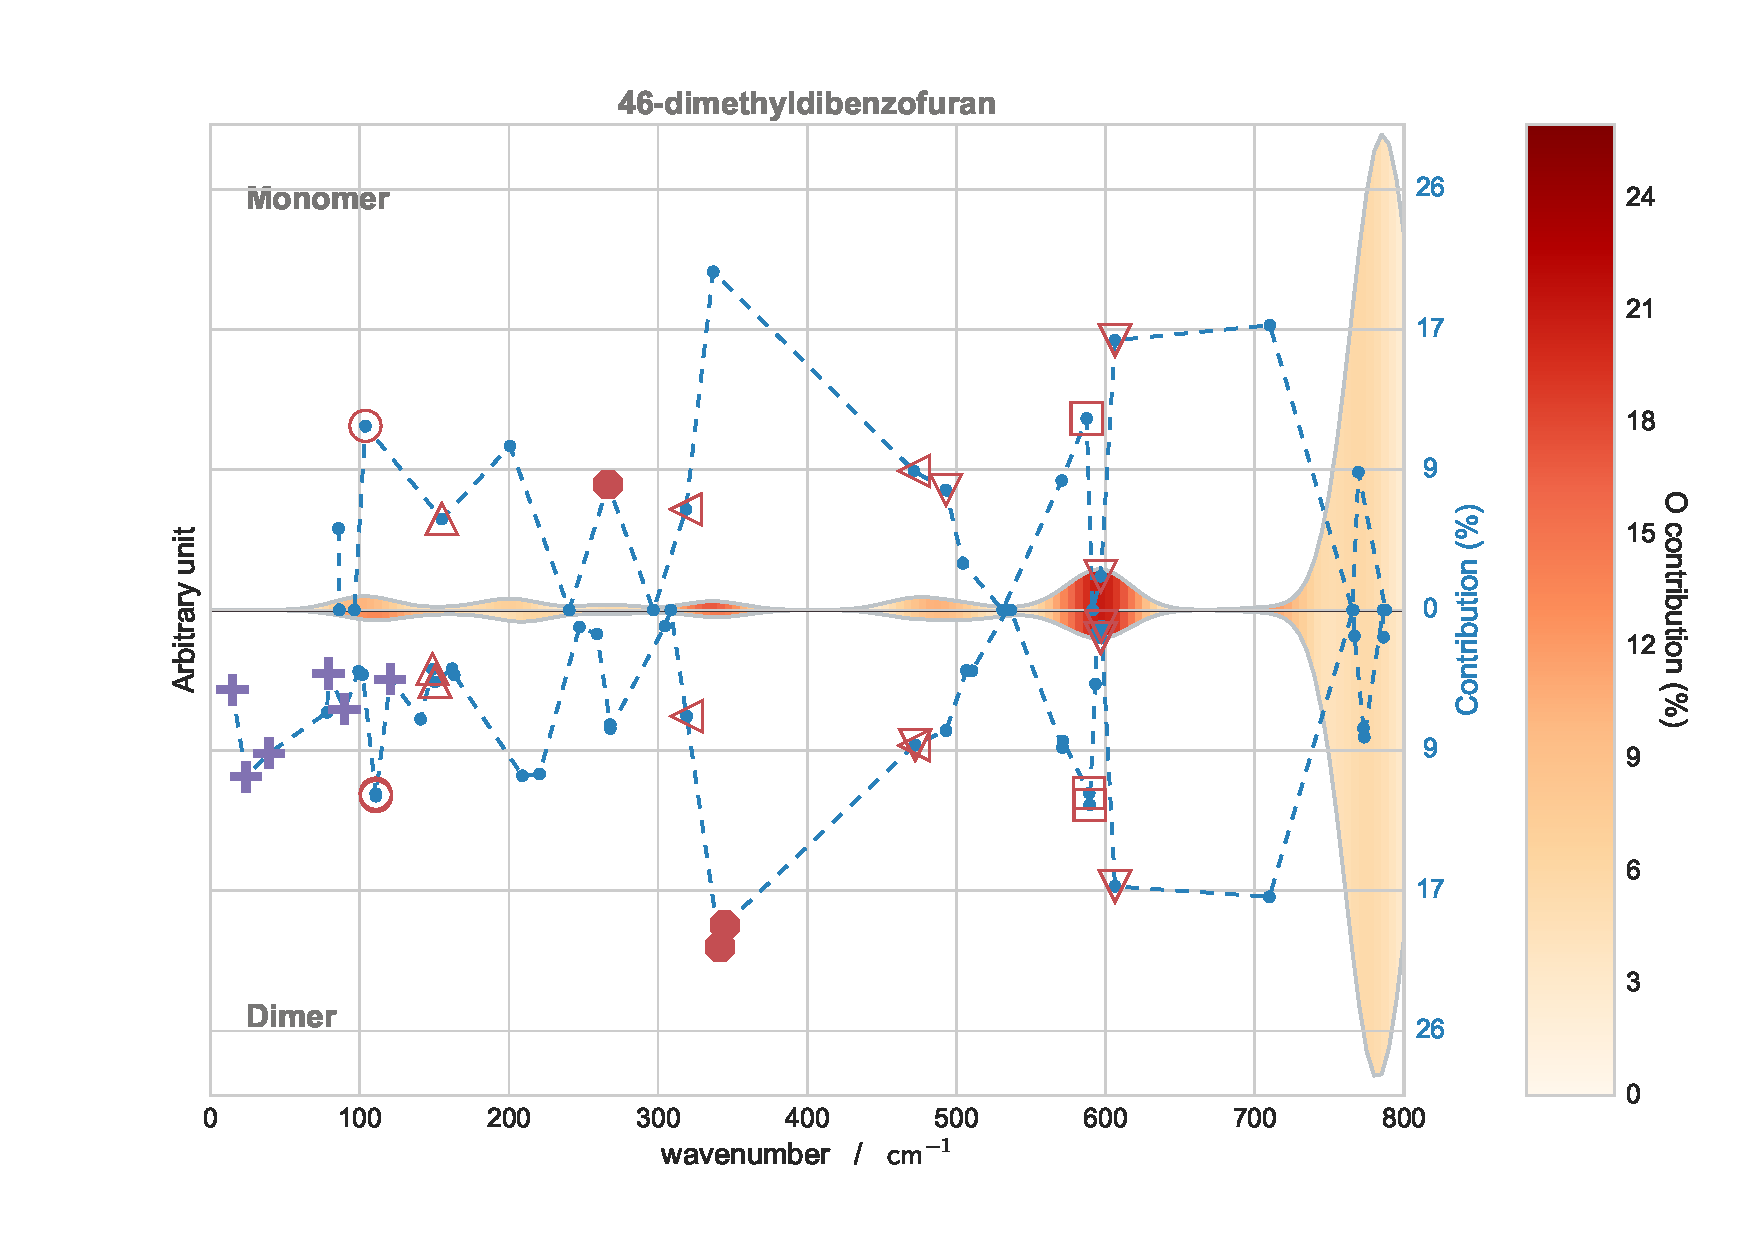
\includegraphics[scale=0.3]{image/P2-17e}\\
				\end{tabular}}
			\end{center}
			\caption{Comparison between momoner and dimer calculated vibrational spectra for \textbf{a} Benzofuran, \textbf{b} Dibenzofuran, \textbf{c} Benzonaphthofuran, \textbf{d} Tribenzofuran, \textbf{e} 4-methyldibenzofuran and \textbf{f} 4,6-dimethyldibenzofuran at 0- 800 cm$^{-1}$ interval.} \label{figP2-17ae}
		\end{figure}
		
		
			\begin{figure}[H]
				\begin{center}
					\resizebox{17cm}{!}{
						\begin{tabular}{c c}
							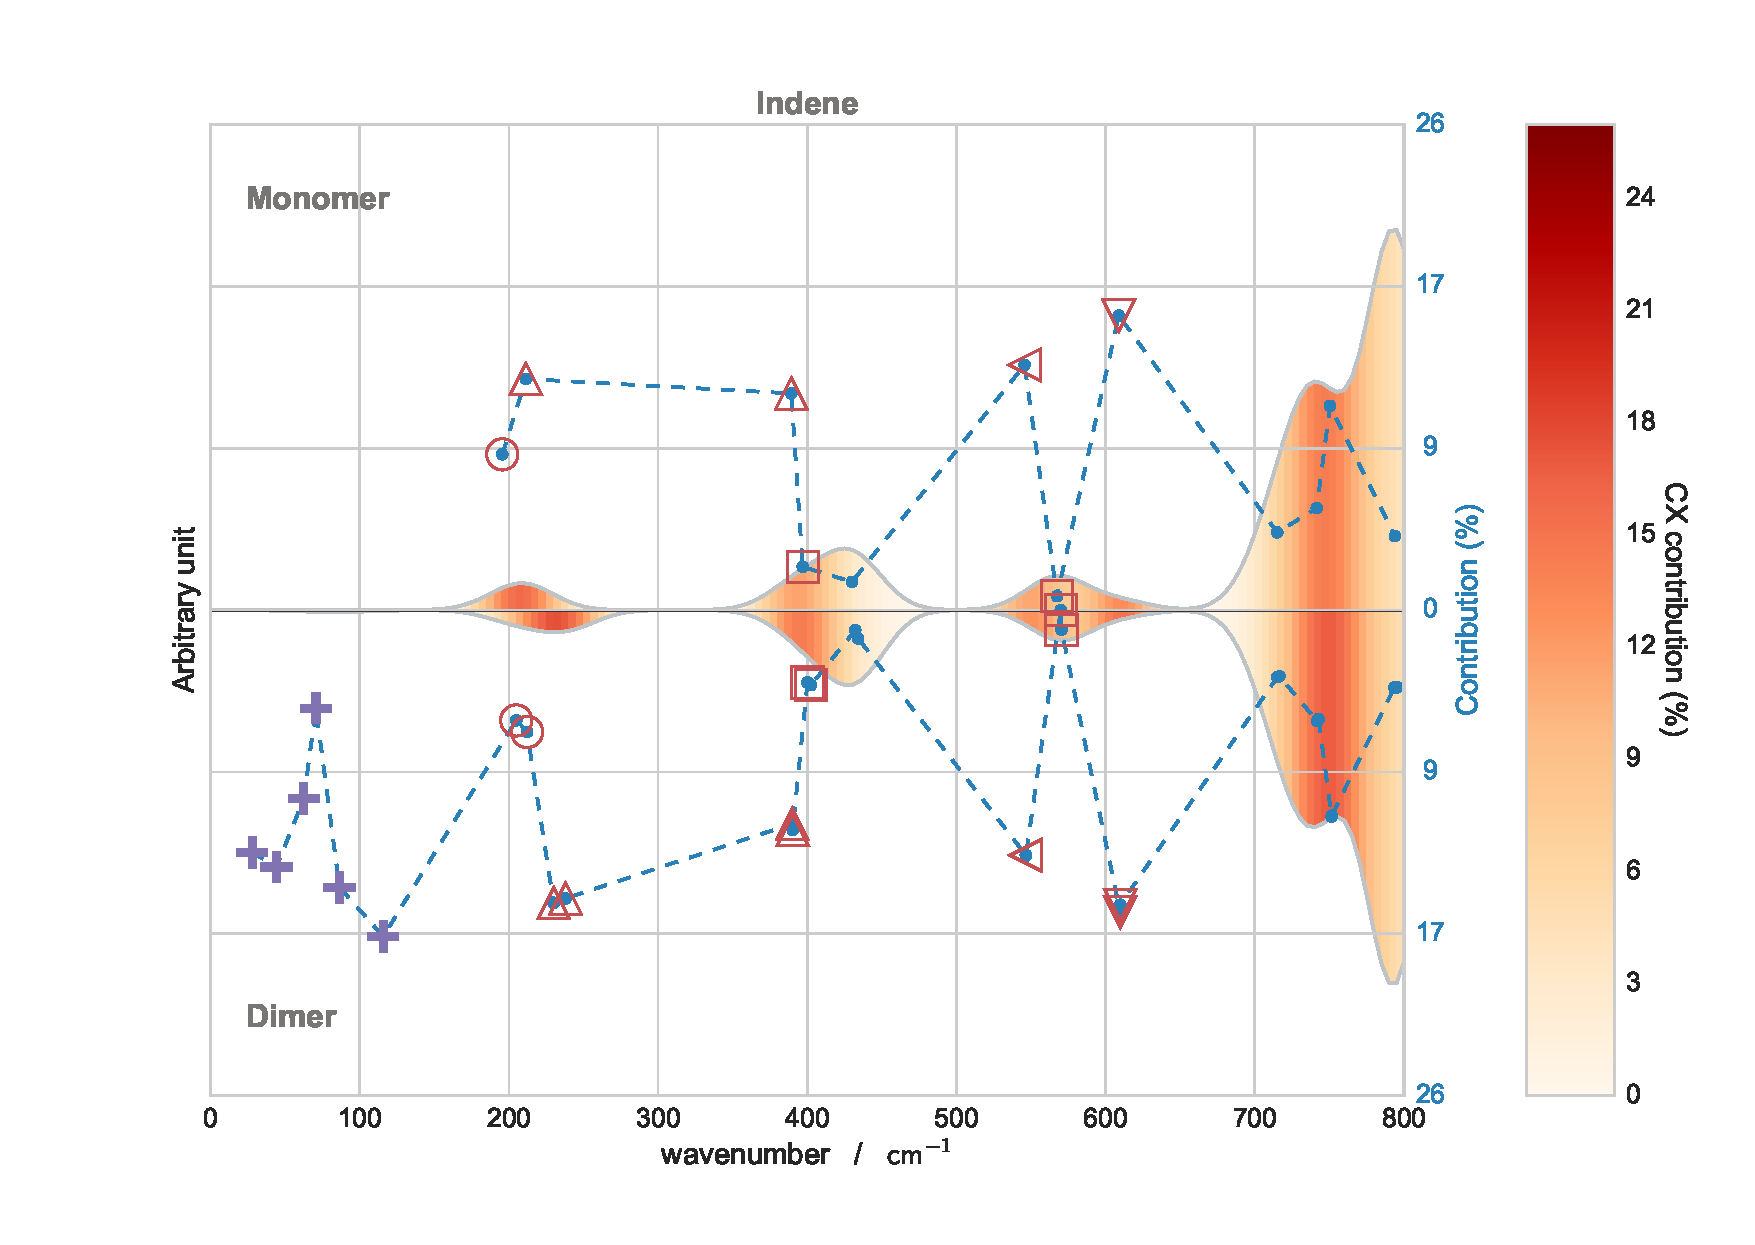
\includegraphics[scale=0.3]{image/P2-18a} & 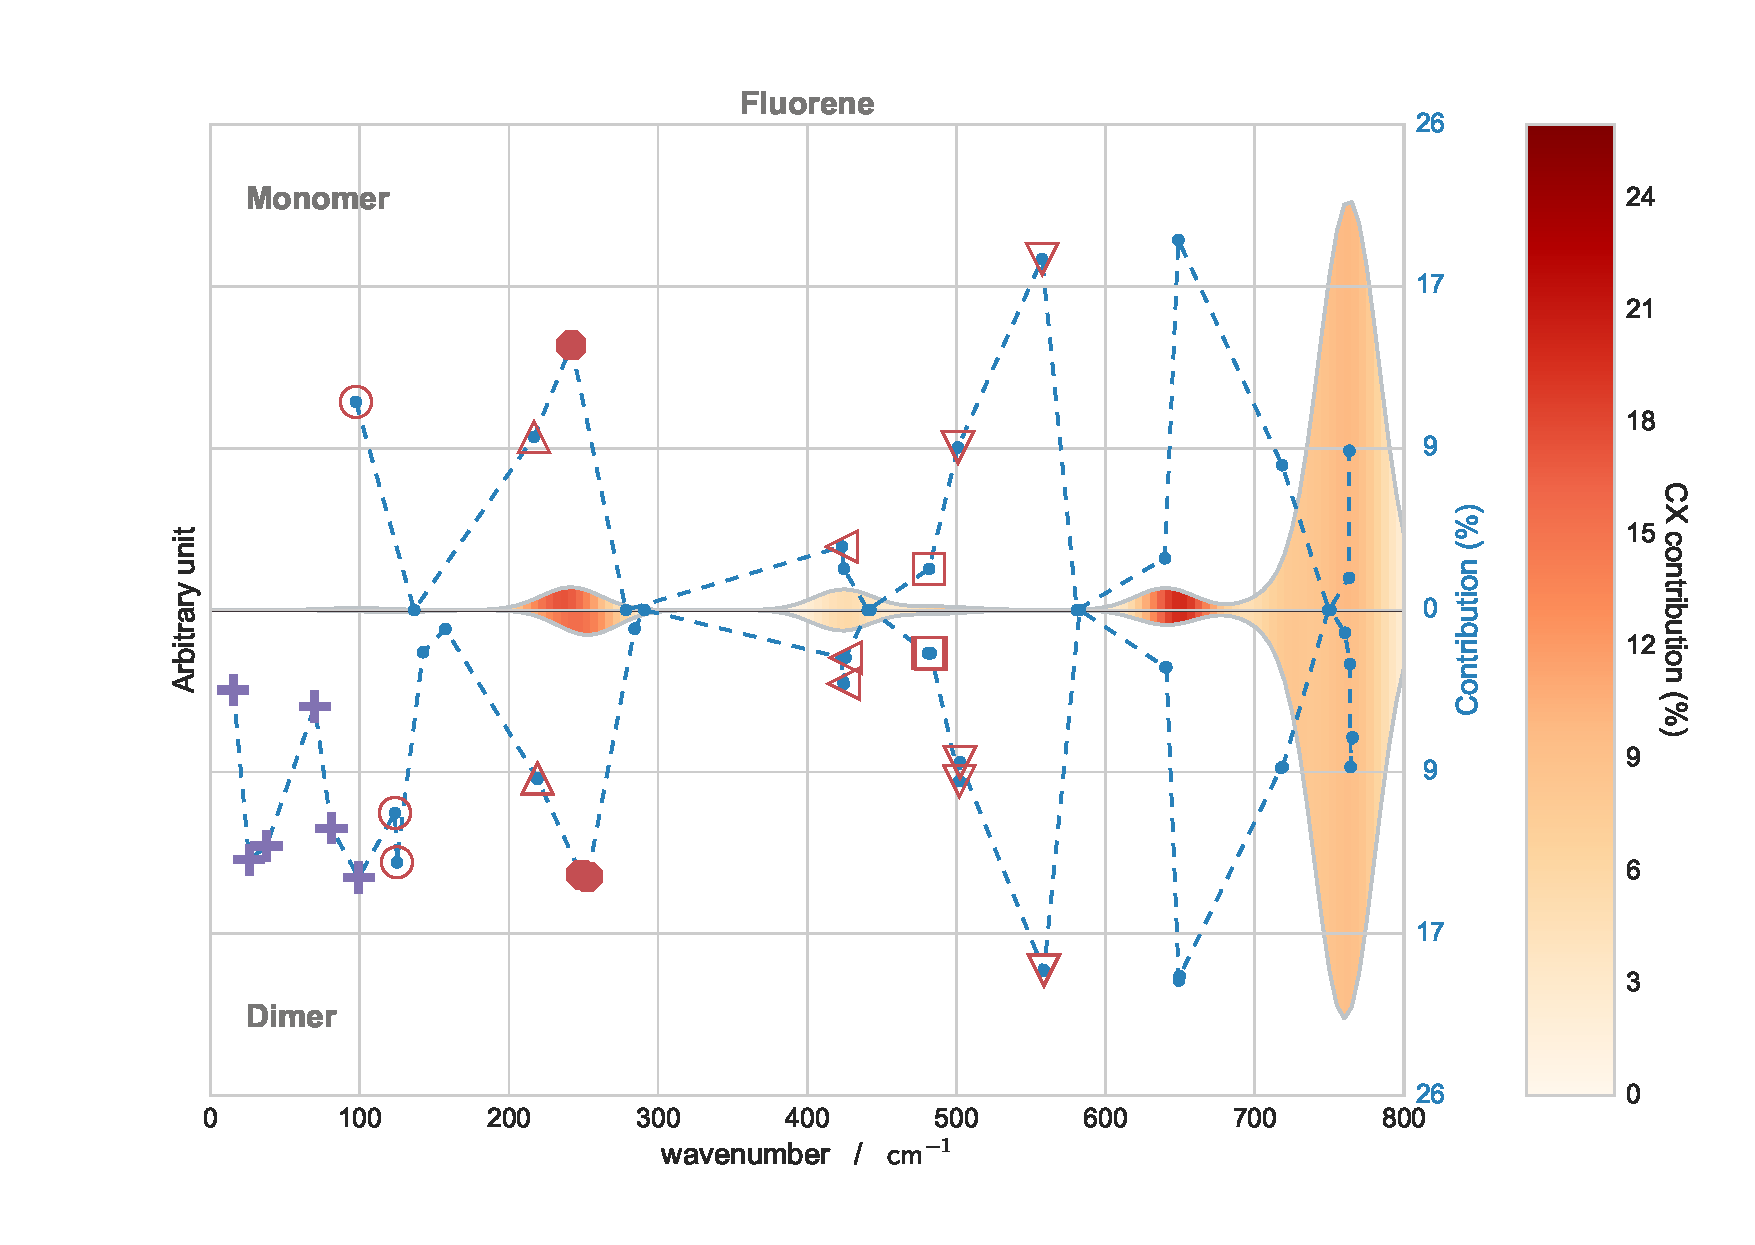
\includegraphics[scale=0.3]{image/P2-18b} \\
							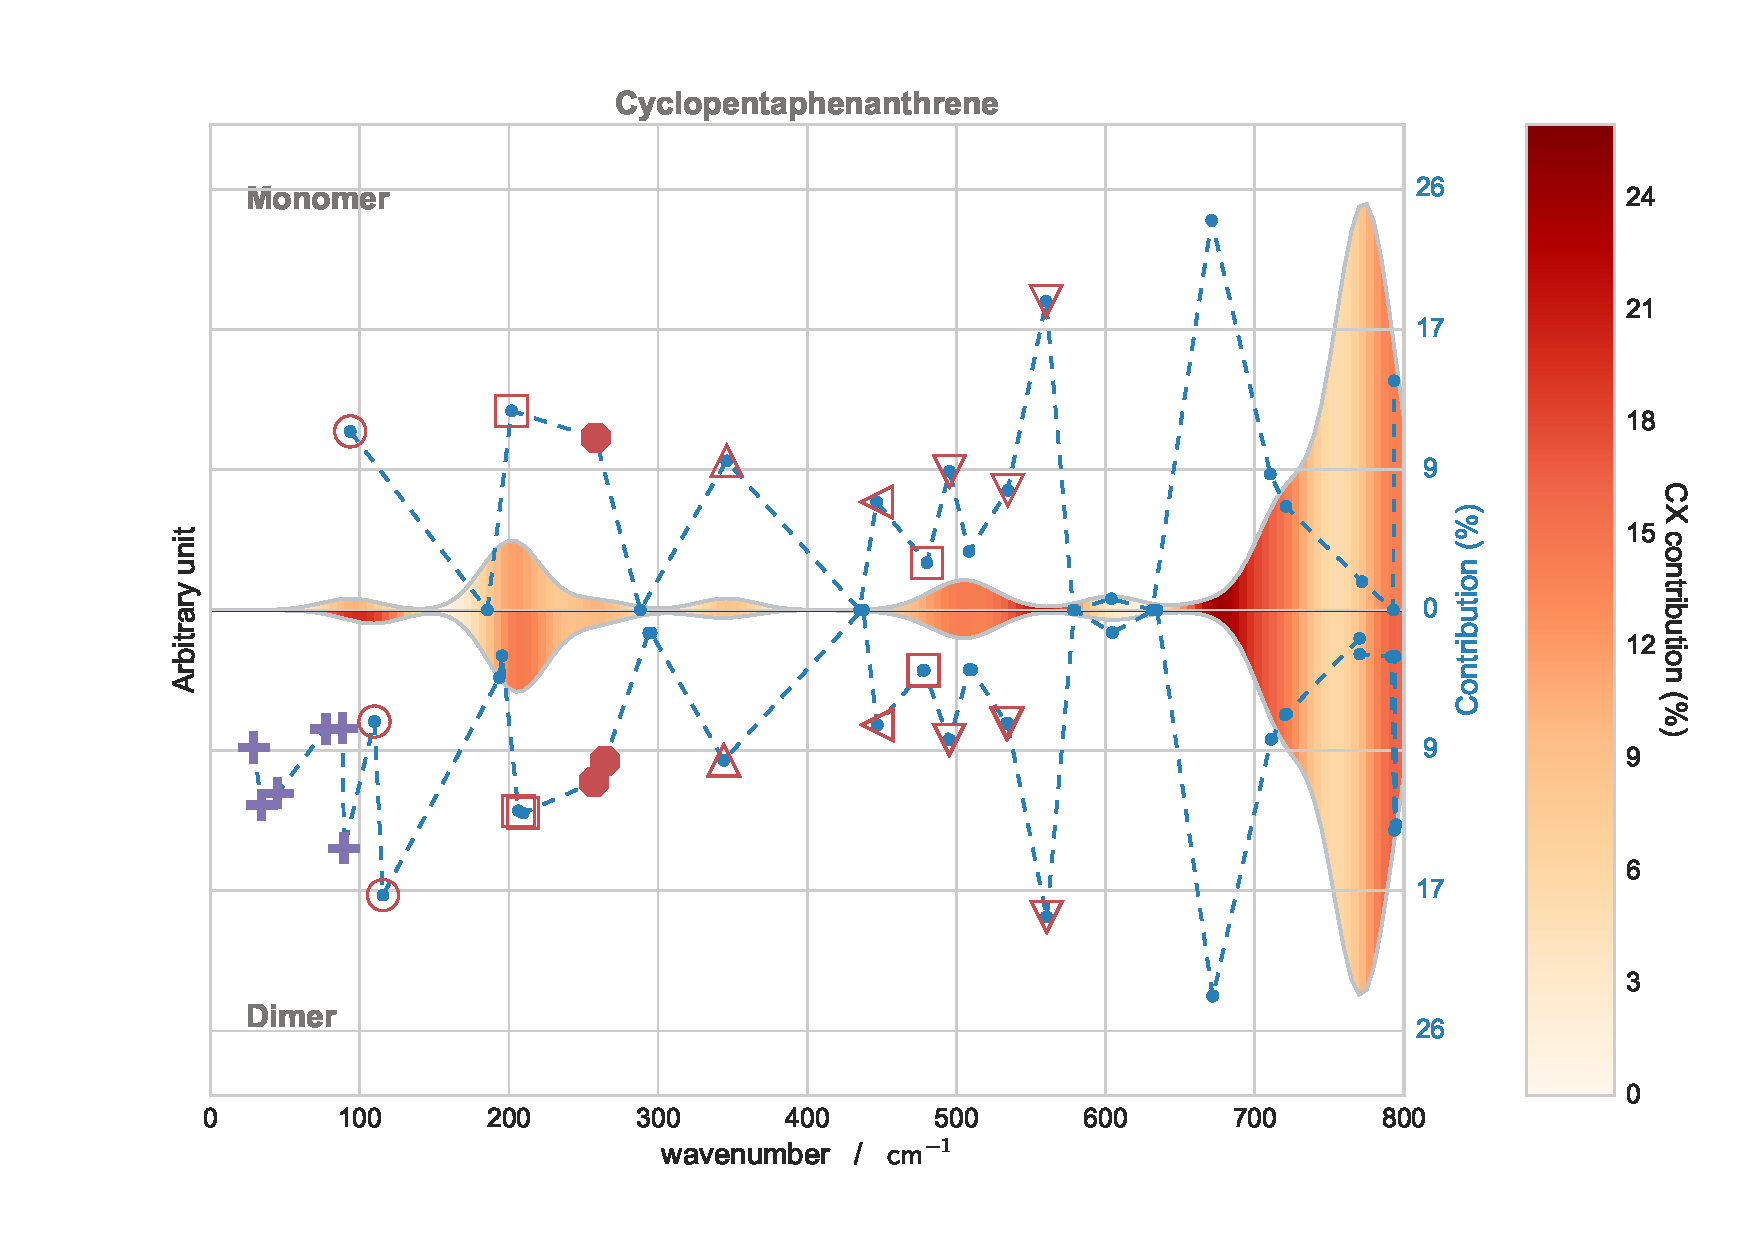
\includegraphics[scale=0.3]{image/P2-18c} & \\ 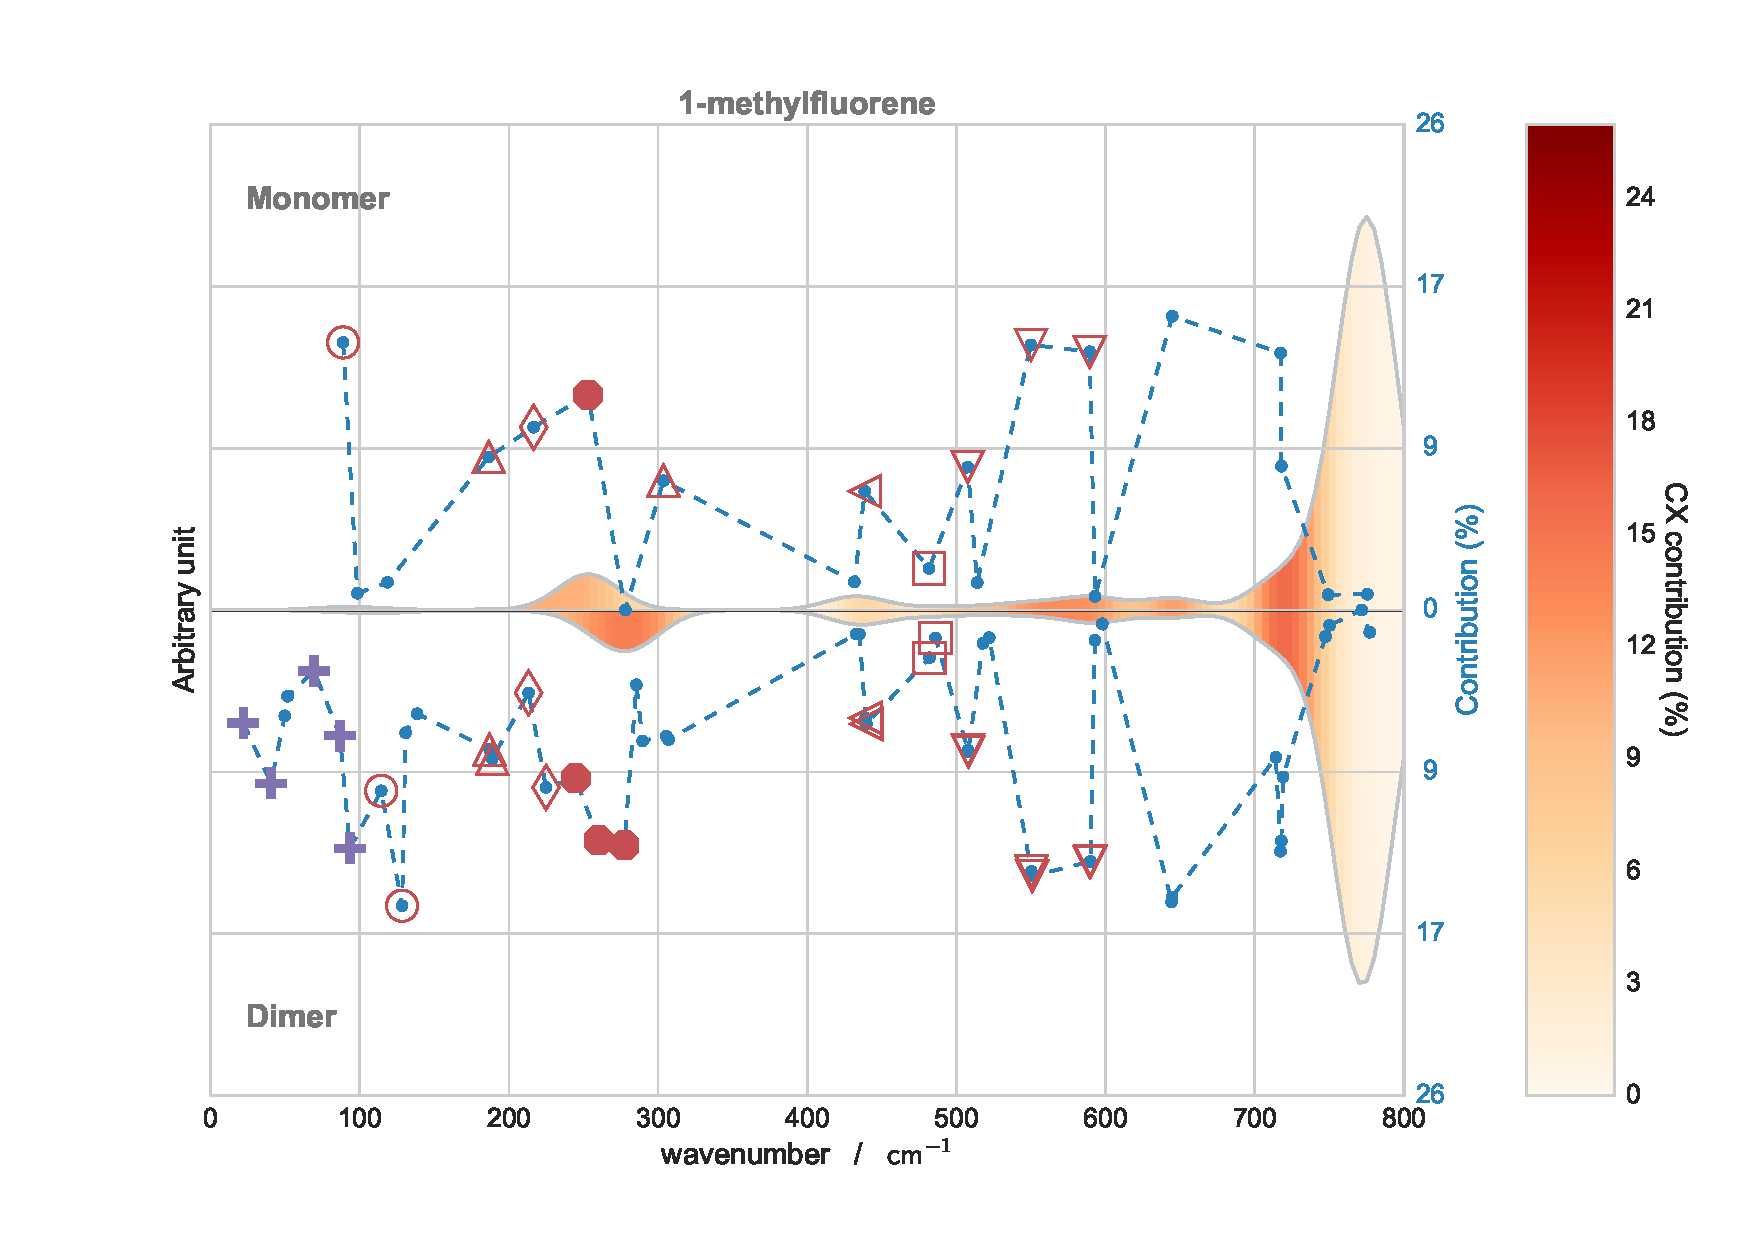
\includegraphics[scale=0.3]{image/P2-18d}&
							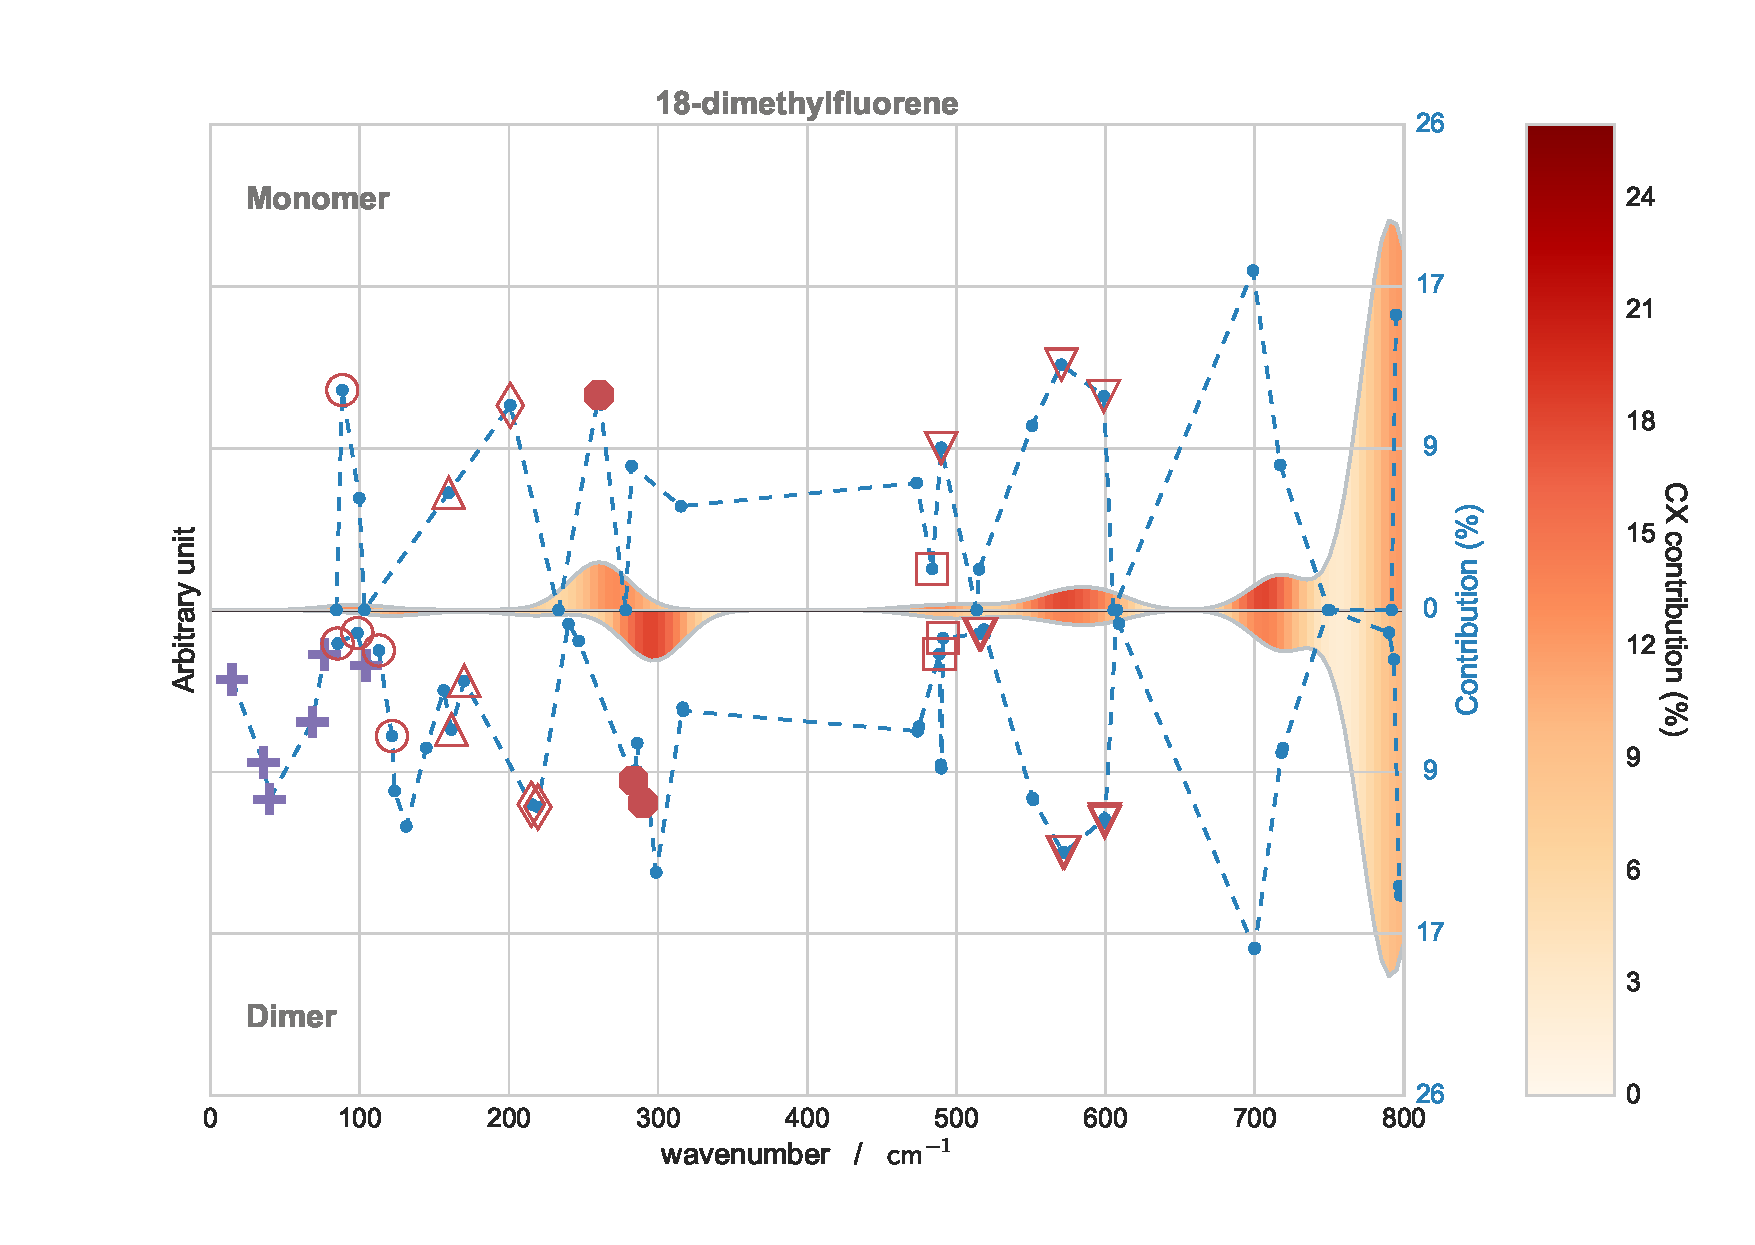
\includegraphics[scale=0.3]{image/P2-18e}  \\
					\end{tabular}}
					\end{center}
					\caption{Comparison between momoner and dimer calculated vibrational spectra for \textbf{a} Indene, \textbf{b} Fluorene, \textbf{c} Cyclopentaphenanthrene, \textbf{d} 1-methylfluorene and \textbf{e} 1,8-dimethylfluorene at 0- 800 cm$^{-1}$ interval.} \label{figP2-18ae}
				\end{figure}
		
		

	
